        %%******************************************%%
        %%                                          %%
        %%        Modello di tesi di laurea         %%
        %%            di Andrea Giraldin            %%
        %%                                          %%
        %%             2 novembre 2012              %%
        %%                                          %%
        %%******************************************%%


% I seguenti commenti speciali impostano:
% 1. 
% 2. PDFLaTeX come motore di composizione;
% 3. tesi.tex come documento principale;
% 4. il controllo ortografico italiano per l'editor.

% !TEX encoding = UTF-8
% !TEX TS-program = pdflatex
% !TEX root = tesi.tex
% !TEX spellcheck = it-IT

\documentclass[10pt,                    % corpo del font principale
               a4paper,                 % carta A4
               twoside,                 % impagina per fronte-retro
               openright,               % inizio capitoli a destra
               english,                 
               english,                 
               ]{book}    

\usepackage[T1]{fontenc}                % codifica dei font:
% NOTA BENE! richiede una distribuzione *completa* di LaTeX

\usepackage[utf8]{inputenc}             % codifica di input; anche [latin1] va bene
                                        % NOTA BENE! va accordata con le preferenze dell'editor

%**************************************************************
% Importazione package
%************************************************************** 

%\usepackage{amsmath,amssymb,amsthm}    % matematica

\usepackage[english]{babel}    % per scrivere in italiano e in inglese;
                                        % l'ultima lingua (l'italiano) risulta predefinita

\usepackage{bookmark}                   % segnalibri

\usepackage{caption}                    % didascalie

\usepackage{chngpage,calc}              % centra il frontespizio

\usepackage{csquotes}                   % gestisce automaticamente i caratteri (")

\usepackage{emptypage}                  % pagine vuote senza testatina e piede di pagina

\usepackage{epigraph}					% per epigrafi

\usepackage{eurosym}                    % simbolo dell'euro



%\usepackage{indentfirst}               % rientra il primo paragrafo di ogni sezione

\usepackage{graphicx}                   % immagini

\usepackage{hyperref}                   % collegamenti ipertestuali

\usepackage[binding=5mm]{layaureo}      % margini ottimizzati per l'A4; rilegatura di 5 mm

\usepackage{listings, lstautogobble}                   % codici

\usepackage{microtype}                  % microtipografia

\usepackage{mparhack,fixltx2e,relsize}  % finezze tipografiche

\usepackage{nameref}                    % visualizza nome dei riferimenti                                      

\usepackage[font=small]{quoting}        % citazioni

\usepackage{subfig}                     % sottofigure, sottotabelle

\usepackage[english]{varioref}          % riferimenti completi della pagina

\usepackage[dvipsnames, table, x11names]{xcolor}         % colori

\usepackage{booktabs}                   % tabelle                                       
\usepackage{tabularx}                   % tabelle di larghezza prefissata                                    
\usepackage{longtable}                  % tabelle su più pagine                                        
%\usepackage{ltxtable}                   % tabelle su più pagine e adattabili in larghezza

\usepackage[toc, acronym]{glossaries}   % glossario
                                        % per includerlo nel documento bisogna:
                                        % 1. compilare una prima volta tesi.tex;
                                        % 2. eseguire: makeindex -s tesi.ist -t tesi.glg -o tesi.gls tesi.glo
                                        % 3. eseguire: makeindex -s tesi.ist -t tesi.alg -o tesi.acr tesi.acn
                                        % 4. compilare due volte tesi.tex.

\usepackage[backend=biber,style=ieee,hyperref]{biblatex}
                                        % eccellente pacchetto per la bibliografia; 
                                        % produce uno stile di citazione autore-anno; 
                                        % lo stile "numeric-comp" produce riferimenti numerici
                                        % per includerlo nel documento bisogna:
                                        % 1. compilare una prima volta tesi.tex;
                                        % 2. eseguire: biber tesi
                                        % 3. compilare ancora tesi.tex.

%**************************************************************
% Pacchetti  e comandi Jordan
%**************************************************************

\usepackage{float}
\usepackage{makecell}
\usepackage{enumitem}
\usepackage{tcolorbox}
\usepackage{booktabs}
%\usepackage[space]{grffile}

\usepackage{ltablex}
\usepackage{tabu}
\usepackage{amssymb}% http://ctan.org/pkg/amssymb
\usepackage{pifont}% http://ctan.org/pkg/pifont
\usepackage{algorithm} 
\usepackage{algpseudocode}
\usepackage{textcomp}
\usepackage{multirow}

\raggedbottom


\definecolor{I}{HTML}{0172CE} %old:0076FF %CornflowerBlue!50
\definecolor{P}{HTML}{FFFFFF}
\definecolor{D}{HTML}{CCE6FF}
\newcolumntype{Y}{>{\centering\arraybackslash}X} % colonna X centrata per tabularx
\renewcommand{\tabularxcolumn}[1]{>{\small}m{#1}}
\newcommand\VRule[1][\arrayrulewidth]{\color{white} \vrule width 1pt}

\newcommand\green[1]{\textcolor{ForestGreen}{#1}} %colore testo 
\newcommand\red[1]{\textcolor{Red}{#1}}
\newcommand\super[0]{\green{S}}
\newcommand\nonsuper[0]{\red{NS}}
\newcommand\impl[0]{\green{I}}
\newcommand\nonimpl[0]{\red{NI}}

\newcommand\greencheck[0]{\green{\ding{51}}}
\newcommand\yellowcheck[0]{\textcolor{YellowOrange}{\ding{51}}}
\newcommand\redx[0]{\red{\ding{55}}}

\newcommand\imgref[1]{\hyperref[#1]{figure \ref{#1}}}
\newcommand\imgrefcap[1]{\hyperref[#1]{Figure \ref{#1}}}

%Extra space in top and bottom tables
\newcommand\Tstrut{\rule{0pt}{2.6ex}}       % "top" strut
\newcommand\Bstrut{\rule[-0.9ex]{0pt}{0pt}} % "bottom" strut
\newcommand{\TBstrut}{\Tstrut\Bstrut} % top&bottom struts

\usepackage{array}
\newcommand{\PreserveBackslash}[1]{\let\temp=\\#1\let\\=\temp}
\newcolumntype{C}[1]{>{\PreserveBackslash\centering}p{#1}}
\newcolumntype{R}[1]{>{\PreserveBackslash\raggedleft}p{#1}}
\newcolumntype{L}[1]{>{\PreserveBackslash\raggedright}p{#1}}

%\lstset{% Add other global options here
%	%basicstyle=\small\sffamily,
%	escapechar=\&,	% char to escape out of listings and back to LaTeX
%	autogobble=true,
%	tabsize=4,
%	numbers=left, numberstyle=\tiny, stepnumber=2, numbersep=5pt
%}

\algnewcommand\algorithmicforeach{\textbf{for each}}
\algdef{S}[FOR]{ForEach}[1]{\algorithmicforeach\ #1\ \algorithmicdo}


%**************************************************************
% file contenente le impostazioni della tesi
%**************************************************************

%**************************************************************
% Frontespizio
%**************************************************************

% Autore
\newcommand{\myName}{Jordan Gottardo}                                    
\newcommand{\myTitle}{Fast Message Propagation Over IoV Scenarios}

% Tipo di tesi                   
\newcommand{\myDegree}{Tesi di laurea magistrale}

% Università             
\newcommand{\myUni}{Università degli Studi di Padova}

% Facoltà       
\newcommand{\myFaculty}{Corso di Laurea in Informatica}

% Dipartimento
\newcommand{\myDepartment}{Dipartimento di Matematica "Tullio Levi-Civita"}

% Titolo del relatore
\newcommand{\profTitle}{Prof. }

% Relatore
\newcommand{\myProf}{Claudio E. Palazzi Armir Bujari}

% Luogo
\newcommand{\myLocation}{Padova}

% Anno accademico
\newcommand{\myAA}{2018-2019}

% Data discussione
\newcommand{\myTime}{18/07/2019}


%**************************************************************
% Impostazioni di impaginazione
% see: http://wwwcdf.pd.infn.it/AppuntiLinux/a2547.htm
%**************************************************************

\setlength{\parindent}{14pt}   % larghezza rientro della prima riga
\setlength{\parskip}{0pt}   % distanza tra i paragrafi


%**************************************************************
% Impostazioni di biblatex
%**************************************************************
\bibliography{bibliografia} % database di biblatex 

\defbibheading{bibliography} {
    \cleardoublepage
    \phantomsection 
    \addcontentsline{toc}{chapter}{\bibname}
    \chapter*{\bibname\markboth{\bibname}{\bibname}}
}

\setlength\bibitemsep{1.5\itemsep} % spazio tra entry

\DeclareBibliographyCategory{opere}
\DeclareBibliographyCategory{web}

\addtocategory{opere}{womak:lean-thinking}
\addtocategory{web}{site:agile-manifesto}

\defbibheading{opere}{\section*{Riferimenti bibliografici}}
\defbibheading{web}{\section*{Siti Web consultati}}


%**************************************************************
% Impostazioni di caption
%**************************************************************
\captionsetup{
    tableposition=top,
    figureposition=bottom,
    font=small,
    format=hang,
    labelfont=bf
}

%**************************************************************
% Impostazioni di glossaries
%**************************************************************

%**************************************************************
% Acronimi
%**************************************************************
\renewcommand{\acronymname}{Acronimi e abbreviazioni}

%\newacronym[description={\glslink{rpma}{rpm}}]{rpma}{RPM}{Radio Propagation Model}
\newacronym{rpma}{RPM}{Radio Propagation Model}
\newacronym{vaneta}{VANET}{Vehicular Ad-Hoc Network}
\newacronym{losa}{LOS}{Line of sight}
\newacronym{nica}{NIC}{Network Interface Controller}
%\newacronym[description={Unified Modeling Language}}]
%{uml}{UML}{Unified Modeling Language}

%**************************************************************
% Glossario
%**************************************************************
%\renewcommand{\glossaryname}{Glossario}

%**************************************************************
% Termini Glossario Jordan
%**************************************************************

%\newglossaryentry{rpmg} {
%	name=\glslink{rpm}{RPM},
%	text=\mbox{JSR 170},
%	sort=rpm,
%	description={Descrizione rpm}
%}


%\newglossaryentry{jsr283} {
%	name=\glslink{jsr283}{JSR 283},
%	text=\mbox{JSR 283},
%	sort=jsr283,
%	description={Java Request Specification rilasciato il 25 settembre 2009. Rispetto a JSR 170, aggiunge (e in alcuni casi rimpiazza) alcune API e funzionalità. È conosciuto anche come \jquote{JCR v2.0 Specifications}}
%}
%
%\newglossaryentry{webapp} {
%	name=\glslink{webapp}{\textit{Web app}},
%	text=\textit{web app},
%	sort=webapp,
%	description={(ing. applicazione web). È un'applicazione fruibile tramite \textit{web browser}}
%}
%
%\newglossaryentry{framework} {
%	name=\glslink{framework}{Framework},
%	text=\textit{framework},
%	sort=framework,
%	description={È un'architettura logica di supporto (spesso un'implementazione logica di un particolare \textit{design pattern}) su cui un \textit{software} può essere progettato e realizzato, spesso facilitandone lo sviluppo da parte del programmatore}
%}
%
%\newglossaryentry{fidelity} {
%	name=\glslink{fidelity}{Fidelity},
%	text=\textit{fidelity},
%	sort=fidelity,
%	description={È un insieme di pratiche attuate da un'organizzazione commerciale per favorire la fidelizzazione della clientela attraverso premi, agevolazioni e altri incentivi all’acquisto come la classica raccolta punti}
%}
%
%\newglossaryentry{NCR} {
%	name=\glslink{NCR}{NCR},
%	text=NCR,
%	sort=NCR,
%	description={Sigla di National Cash Register. È un'azienda fondata nel 1884 che attualmente opera in gran parte del mondo con soluzioni \textit{retail} e \textit{financial}. Ha sede principale a Dayton (Ohio), U.S.A.; la sede italiana è situata a Milano. Produce principalmente ATM e registratori di cassa}
%}
%
%\newglossaryentry{POS} {
%	name=\glslink{POS}{POS},
%	text=POS,
%	sort=POS,
%	description={(ing. POS, \textit{Point of Sale}). È il dispositivo elettronico che permette di effettuare pagamenti mediante moneta elettronica, ovvero tramite carte di credito, di debito e prepagate}
%}
%
%\newglossaryentry{retail} {
%	name=\glslink{retail}{\textit{Retail}},
%	text=\textit{retail},
%	sort=retail,
%	description={(ing. vendita al dettaglio). È una locuzione utilizzata in ambito commerciale per indicare la vendita di prodotti al consumatore finale. È l'ultimo anello della catena di distribuzione, che inizia dal produttore e può passare per un certo numero di grossisti}
%}
%
%\newglossaryentry{GDO} {
%	name=\glslink{GDO}{GDO},
%	text=GDO,
%	sort=GDO,
%	description={Sigla di Grande Distribuzione Organizzata. Si riferisce al moderno sistema di vendita al dettaglio attraverso una rete di supermercati e ipermercati e di altre catene di intermediari di varia natura. Rappresenta l'evoluzione del supermercato singolo, che a sua volta costituisce lo sviluppo del negozio tradizionale}
%}
%
%\newglossaryentry{clickandcollect} {
%	name=\glslink{clickandcollect}{Click \& collect},
%	text=\textit{click \& collect},
%	sort=click\&collect,
%	description={(ing. prenota e ritira). Metodo di vendita al dettaglio che consiste nella prenotazione, solitamente via \textit{web}, del prodotto da parte del cliente e nel successivo ritiro quando viene segnalata la disponibilità della merce ordinata. La differenza con l'\textit{e-commerce} classico è che la spedizione (in questo caso il ritiro) viene effettuata direttamente dal cliente, senza l'ausilio di corrieri}
%}
%
%\newglossaryentry{pda} {
%	name=\glslink{pda}{PDA},
%	text=PDA,
%	sort=PDA,
%	description={Sigla di \textit{Personal Digital Assistant}. Indica un computer palmare, ovvero un computer di dimensioni talmente contenute da poter essere portato sul palmo di una mano. Lo schermo del PDA è tattile, in modo da permettere l'interazione con le dita o con un apposito pennino}
%}
%
%\newglossaryentry{backoffice} {
%	name=\glslink{backoffice}{\textit{Back office}},
%	text=\textit{back office},
%	sort=backoffice,
%	description={(ing. dietro ufficio, nel significato di retro-ufficio). Termine che indica la parte di azienda che comprende le attività di gestione operativa, amministrativa e tutte le attività che non riguardano direttamente il cliente}
%}
%
%\newglossaryentry{opensource} {
%	name=\glslink{opensource}{\textit{Open source}},
%	text=\textit{open source},
%	sort=opensource,
%	description={(ing. sorgente aperta). È un termine che indica un \textit{software} di cui i detentori dei diritti rendono pubblico il codice sorgente. Così facendo, altri programmatori possono studiare il codice e apportarvi liberamente modifiche ed estensioni}
%}
%
%\newglossaryentry{webservice} {
%	name=\glslink{webservice}{\textit{Web service}},
%	text=\textit{web service},
%	sort=webservice,
%	description={Tipo di architettura \textit{software} che si basa sulla comunicazione tra sistemi distribuiti. La comunicazione solitamente avviene solitamente utilizzando linguaggi come XML e JSON, con messaggi trasportati da protocolli \textit{web} (da cui il nome), come HTTP}
%}
%
%\newglossaryentry{proofofconcept} {
%	name=\glslink{proofofconcept}{\textit{Proof of concept}},
%	text=\textit{proof of concept},
%	sort=proofofconcept,
%	description={(ing. prova del concetto). Termine che indica un prototipo o un'incompleta realizzazione di un progetto, in modo da poterne dimostrare la sua fattibilità}
%}
%
%\newglossaryentry{jackrabbit} {
%	name=\glslink{jackrabbit}{Jackrabbit},
%	text=Jackrabbit,
%	sort=jackrabbit,
%	description={Apache Jackrabbit è una libreria Java open source che fornisce un'implementazione di un Java Content Repository, così come definito dagli standard JSR 170 e JSR 283}
%}
%
%\newglossaryentry{gui} {
%	name=\glslink{gui}{\textit{GUI}},
%	text=GUI,
%	sort=gui,
%	description={(ing. \textit{Graphical User Interface}, interfaccia grafica utente). Indica l'interfaccia con cui l'utente interagisce con un \textit{software} attraverso il controllo di oggetti grafici convenzionali}
%}
%
%\newglossaryentry{javaee} {
%	name=\glslink{javaee}{Java EE},
%	text=Java EE,
%	sort=javaee,
%	description={Java Platform, Enterprise Edition. È una specifica impiegata nello sviluppo di applicazioni \textit{web} in linguaggio Java. Inizialmente, la specifica puntava verso la creazione di applicazioni con architetture \textit{multi-tier}, ma grazie alle recenti evoluzioni permette anche di creare applicazioni basate su microservizi}
%}
%
%\newglossaryentry{swe} {
%	name=\glslink{swe}{Ingegneria del \textit{software}},
%	text=Ingegneria del \textit{software},
%	sort=ingegneriadelsoftware,
%	description={Corso della Laurea Triennale in Informatica di Padova che richiede lo sviluppo di un impegnativo progetto didattico di gruppo secondo canoni rigorosi di gestione del rapporto cliente-fornitore}
%}
%
%\newglossaryentry{fulltext} {
%	name=\glslink{fulltext}{\textit{Full-text}},
%	text=\textit{full-text},
%	sort=fulltext,
%	description={(ing. testo intero). Indica un tipo di ricerca testuale all'interno di un documento o di un \textit{database} in cui il motore di ricerca esamina tutte le parole memorizzate e tenta di trovare un riscontro secondo determinate parole fornite dall'utente}
%}
%
%\newglossaryentry{stakeholder} {
%	name=\glslink{stakeholder}{\textit{Stakeholder}},
%	text=\textit{stakeholder},
%	sort=stakeholder,
%	description={(ing. portatore di interessi). In economia, indica un soggetto che esercita influenza nei confronti di un'attività economica, come ad esempio un progetto}
%}
%
%\newglossaryentry{stub} {
%	name=\glslink{stub}{\textit{Stub}},
%	text=\textit{stub},
%	sort=stub,
%	description={(ing. abbozzo). Indica una porzione di codice utilizzata in sostituzione di altre funzionalità \textit{software}. È utilizzato sopratutto durante l'esecuzione dei \textit{test} per simulare il comportamento di codice su cui non si sta eseguendo il \textit{test}}
%}
%
%\newglossaryentry{statementcoverage} {
%	name=\glslink{statementcoverage}{\textit{Statement coverage}},
%	text=\textit{Statement coverage},
%	sort=statementcoverage,
%	description={(ing. copertura delle dichiarazioni). Indica il grado di codice sorgente che viene eseguito durante l'attuazione dei \textit{test}}
%}
%
%\newglossaryentry{branchcoverage} {
%	name=\glslink{branchcoverage}{\textit{Branch coverage}},
%	text=\textit{Branch coverage},
%	sort=branchcoverage,
%	description={(ing. copertura dei rami). Indica il grado di cammini logici all'interno di un programma coperti durante l'esecuzione dei \textit{test}}
%}
%
%\newglossaryentry{incrementi} {
%	name=\glslink{incrementi}{Incremento},
%	text=\textit{incrementi},
%	sort=incrementi,
%	description={Nel modello incrementale, un incremento è un aumento tangibile di valore del \textit{software} in fase di sviluppo. Il caso più comune di incremento è l'introduzione di nuove funzionalità. Un incremento, per essere tale, deve essere validato internamente}
%}
%
%%**************************************************************
%% Termini Glossario esempio
%%**************************************************************
%
%%\newglossaryentry{apig}
%%{
%%    name=\glslink{api}{API},
%%    text=Application Program Interface,
%%    sort=api,
%%    description={in informatica con il termine \emph{Application Programming Interface API} (ing. interfaccia di programmazione di un'applicazione) si indica ogni insieme di procedure disponibili al programmatore, di solito raggruppate a formare un set di strumenti specifici per l'espletamento di un determinato compito all'interno di un certo programma. La finalità è ottenere un'astrazione, di solito tra l'hardware e il programmatore o tra \textit{software} a basso e quello ad alto livello semplificando così il lavoro di programmazione}
%%}
%
%
%%\newglossaryentry{umlg}
%%{
%%    name=\glslink{uml}{UML},
%%    text=UML,
%%    sort=uml,
%%    description={in ingegneria del \textit{software} \emph{UML, Unified Modeling Language} (ing. linguaggio di modellazione unificato) è un linguaggio di modellazione e specifica basato sul paradigma object-oriented. L'\emph{UML} svolge un'importantissima funzione di ``lingua franca'' nella comunità della progettazione e programmazione a oggetti. Gran parte della letteratura di settore usa tale linguaggio per descrivere soluzioni analitiche e progettuali in modo sintetico e comprensibile a un vasto pubblico}
%%}
 % database di termini
\makeglossaries


%**************************************************************
% Impostazioni di graphicx
%**************************************************************
\graphicspath{{immagini/}} % cartella dove sono riposte le immagini


%**************************************************************
% Impostazioni di hyperref
%**************************************************************
\hypersetup{
    %hyperfootnotes=false,
    %pdfpagelabels,
    %draft,	% = elimina tutti i link (utile per stampe in bianco e nero)
    colorlinks=true,
    linktocpage=true,
    pdfstartpage=1,
    pdfstartview=FitV,
    % decommenta la riga seguente per avere link in nero (per esempio per la stampa in bianco e nero)
    %colorlinks=false, linktocpage=false, pdfborder={0 0 0}, pdfstartpage=1, pdfstartview=FitV,
    breaklinks=true,
    pdfpagemode=UseNone,
    pageanchor=true,
    pdfpagemode=UseOutlines,
    plainpages=false,
    bookmarksnumbered,
    bookmarksopen=true,
    bookmarksopenlevel=1,
    hypertexnames=true,
    pdfhighlight=/O,
    %nesting=true,
    %frenchlinks,
    urlcolor=webbrown,
    linkcolor=RoyalBlue,
    citecolor=webgreen,
    %pagecolor=RoyalBlue,
    %urlcolor=Black, linkcolor=Black, citecolor=Black, %pagecolor=Black,
    pdftitle={\myTitle},
    pdfauthor={\textcopyright\ \myName, \myUni, \myFaculty},
    pdfsubject={},
    pdfkeywords={},
    pdfcreator={pdfLaTeX},
    pdfproducer={LaTeX}
}

%**************************************************************
% Impostazioni di itemize
%**************************************************************
\renewcommand{\labelitemi}{$\ast$}

%\renewcommand{\labelitemi}{$\bullet$}
%\renewcommand{\labelitemii}{$\cdot$}
%\renewcommand{\labelitemiii}{$\diamond$}
%\renewcommand{\labelitemiv}{$\ast$}


%**************************************************************
% Impostazioni di listings
%**************************************************************
\lstset{
    language=[LaTeX]Tex,%C++,
    keywordstyle=\color{RoyalBlue}, %\bfseries,
    basicstyle=\small\ttfamily,
    %identifierstyle=\color{NavyBlue},
    commentstyle=\color{Green}\ttfamily,
    stringstyle=\rmfamily,
    numbers=none, %left,%
    numberstyle=\scriptsize, %\tiny
    stepnumber=5,
    numbersep=8pt,
    showstringspaces=false,
    breaklines=true,
    frameround=ftff,
    frame=single
} 


%**************************************************************
% Impostazioni di xcolor
%**************************************************************
\definecolor{webgreen}{rgb}{0,.5,0}
\definecolor{webbrown}{rgb}{.6,0,0}


%**************************************************************
% Altro
%**************************************************************

\newcommand{\omissis}{[\dots\negthinspace]} % produce [...]

% eccezioni all'algoritmo di sillabazione
\hyphenation
{
    ma-cro-istru-zio-ne
    gi-ral-din
}

\newcommand{\sectionname}{sezione}
\addto\captionsitalian{\renewcommand{\figurename}{Figura}
                       \renewcommand{\tablename}{Tabella}}

\newcommand{\glsfirstoccur}{\ap{{[g]}}}

\newcommand{\intro}[1]{\emph{\textsf{#1}}}

%**************************************************************
% Environment per ``rischi''
%**************************************************************
\newcounter{riskcounter}                % define a counter
\setcounter{riskcounter}{0}             % set the counter to some initial value

%%%% Parameters
% #1: Title
\newenvironment{risk}[1]{
    \refstepcounter{riskcounter}        % increment counter
    \par \noindent                      % start new paragraph
    \textbf{\arabic{riskcounter}. #1}   % display the title before the 
                                        % content of the environment is displayed 
}{
    \par\medskip
}

\newcommand{\riskname}{Rischio}

\newcommand{\riskdescription}[1]{\textbf{\\Descrizione:} #1.}

\newcommand{\risksolution}[1]{\textbf{\\Soluzione:} #1.}

%**************************************************************
% Environment per ``use case''
%**************************************************************
\newcounter{usecasecounter}             % define a counter
\setcounter{usecasecounter}{0}          % set the counter to some initial value

%%%% Parameters
% #1: ID
% #2: Nome
\newenvironment{usecase}[2]{
    \renewcommand{\theusecasecounter}{\usecasename #1}  % this is where the display of 
                                                        % the counter is overwritten/modified
    \refstepcounter{usecasecounter}             % increment counter
    \vspace{10pt}
    \par \noindent                              % start new paragraph
    {\large \textbf{\usecasename #1: #2}}       % display the title before the 
                                                % content of the environment is displayed 
    \medskip
}{
    \medskip
}

\newcommand{\usecasename}{UC}

\newcommand{\usecaseactors}[1]{\textbf{\\Attori Principali:} #1. \vspace{4pt}}
\newcommand{\usecasepre}[1]{\textbf{\\Precondizioni:} #1. \vspace{4pt}}
\newcommand{\usecasedesc}[1]{\textbf{\\Descrizione:} #1. \vspace{4pt}}
\newcommand{\usecasepost}[1]{\textbf{\\Postcondizioni:} #1. \vspace{4pt}}
\newcommand{\usecasealt}[1]{\textbf{\\Scenario Alternativo:} #1. \vspace{4pt}}

%**************************************************************
% Environment per ``namespace description''
%**************************************************************

\newenvironment{namespacedesc}{
    \vspace{10pt}
    \par \noindent                              % start new paragraph
    \begin{description} 
}{
    \end{description}
    \medskip
}

\newcommand{\classdesc}[2]{\item[\textbf{#1:}] #2}

%**************************************************************
% Comandi Jordan
%**************************************************************

\newcommand{\jquote}[1]{“#1”}                     % file con le impostazioni personali

\begin{document}
%**************************************************************
% Materiale iniziale
%**************************************************************
\frontmatter
% !TEX encoding = UTF-8
% !TEX TS-program = pdflatex
% !TEX root = ../tesi.tex

%**************************************************************
% Frontespizio 
%**************************************************************
\begin{titlepage}

\begin{center}

\begin{LARGE}
\textbf{\myUni}\\
\end{LARGE}

\vspace{10pt}

\begin{Large}
\textsc{\myDepartment}\\
\end{Large}

\vspace{10pt}

\begin{large}
\textsc{\myFaculty}\\
\end{large}

\vspace{30pt}
\begin{figure}[htbp]
\begin{center}

\includegraphics[height=6cm]{logo-unipd}
\end{center}
\end{figure}
\vspace{30pt} 

\begin{LARGE}
\begin{center}
\textbf{\myTitle}\\
\end{center}
\end{LARGE}

\vspace{10pt} 

\begin{large}
\textsl{\myDegree}\\
\end{large}

\vspace{40pt} 

\begin{large}
\begin{flushleft}
\textit{Relatore}\\ 
\vspace{5pt} 
\profTitle \myProf
\end{flushleft}

\vspace{0pt} 

\begin{flushright}
\textit{Laureando}\\ 
\vspace{5pt} 
\myName
\end{flushright}
\end{large}

\vspace{40pt}

\line(1, 0){338} \\
\begin{normalsize}
\textsc{Anno Accademico \myAA}
\end{normalsize}

\end{center}
\end{titlepage} 
% !TEX encoding = UTF-8
% !TEX TS-program = pdflatex
% !TEX root = ../tesi.tex

%**************************************************************
% Colophon
%**************************************************************
\clearpage
\phantomsection
\thispagestyle{empty}

\hfill

\vfill

\noindent\myName: \textit{\myTitle,}
\myDegree,
\textcopyright\ \myTime.
%% !TEX encoding = UTF-8
% !TEX TS-program = pdflatex
% !TEX root = ../tesi.tex

%**************************************************************
% Dedica
%**************************************************************
\cleardoublepage
\phantomsection
\thispagestyle{empty}
\pdfbookmark{Dedica}{Dedica}

\vspace*{3cm}

\begin{center}
Lorem ipsum dolor sit amet, consectetuer adipiscing elit. \\ \medskip
--- Oscar Wilde    
\end{center}

\medskip

\begin{center}
Dedicato a ...
\end{center}

% !TEX encoding = UTF-8
% !TEX TS-program = pdflatex
% !TEX root = ../tesi.tex

%**************************************************************
% Sommario
%**************************************************************
\cleardoublepage
\phantomsection
\pdfbookmark{Abstract}{Abstract}
\begingroup
\let\clearpage\relax
\let\cleardoublepage\relax
\let\cleardoublepage\relax

\chapter*{Abstract}

The increasingly pervasive use of technology in the automotive industry and urban environment requires the development of broadcasting algorithms to deliver messages across vehicular ad-hoc networks (VANETs). These kinds of networks are created spontaneously and rely on vehicle-to-vehicle communication, without the need of any infrastructure or prior network topology knowledge by nodes. It is foreseeable that, in the near future, VANETs could be exploited in order to run heterogeneous applications, ranging from leisure-oriented functionalities such as video streaming and gaming, to more serious data exchanging services to monitor traffic congestion. One important application consists in emergency message distribution, where message delivery, timeliness and other life-safety related metrics are paramount. Whereas most of related work in this field is focused on one-dimensional topologies (i.e., car platooning in highways), this thesis consists in the reimplementation and redesign for two and three-dimensional scenarios of the RObust and Fast Forwarding algorithm (ROFF) and the Fast-Broadcast algorithm to compare them in various urban scenarios of increasing complexity. Considering urban scenarios, the Obstacle Model will be employed to take into account the shadowing effects of buildings on signal propagation. Moreover, this thesis proposes a Smart Junction extension for both algorithms, SJ-Fast-Broadcast and SJ-ROFF, which increase message delivery ratios by exploiting the presence of vehicles within road junctions in scenarios where the shadowing effects of obstacles is significant.

\endgroup			

\vfill


%% !TEX encoding = UTF-8
% !TEX TS-program = pdflatex
% !TEX root = ../tesi.tex

%**************************************************************
% Ringraziamenti
%**************************************************************
\cleardoublepage
\phantomsection
\pdfbookmark{Ringraziamenti}{ringraziamenti}

\begin{flushright}{
	\slshape    
	``Life is really simple, but we insist on making it complicated''} \\ 
	\medskip
    --- Confucius
\end{flushright}


\bigskip

\begingroup
\let\clearpage\relax
\let\cleardoublepage\relax
\let\cleardoublepage\relax

\chapter*{Ringraziamenti}

\noindent \textit{Innanzitutto, vorrei esprimere la mia gratitudine al Prof. NomeDelProfessore, relatore della mia tesi, per l'aiuto e il sostegno fornitomi durante la stesura del lavoro.}\\

\noindent \textit{Desidero ringraziare con affetto i miei genitori per il sostegno, il grande aiuto e per essermi stati vicini in ogni momento durante gli anni di studio.}\\

\noindent \textit{Ho desiderio di ringraziare poi i miei amici per tutti i bellissimi anni passati insieme e le mille avventure vissute.}\\
\bigskip

\noindent\textit{\myLocation, \myTime}
\hfill \myName

\endgroup


% !TEX encoding = UTF-8
% !TEX TS-program = pdflatex
% !TEX root = ../tesi.tex

%**************************************************************
% Indici
%**************************************************************
\cleardoublepage
\pdfbookmark{\contentsname}{tableofcontents}
\setcounter{tocdepth}{2}
\tableofcontents
%\markboth{\contentsname}{\contentsname} 
\clearpage

\begingroup 
    \let\clearpage\relax
    \let\cleardoublepage\relax
    \let\cleardoublepage\relax
    %*******************************************************
    % Elenco delle figure
    %*******************************************************    
    \phantomsection
    \pdfbookmark{\listfigurename}{lof}
    \listoffigures

    \vspace*{8ex}

    %*******************************************************
    % Elenco delle tabelle
    %*******************************************************
    \phantomsection
    \pdfbookmark{\listtablename}{lot}
    \listoftables
        
    \vspace*{8ex}
\endgroup

\cleardoublepage

\cleardoublepage

%**************************************************************
% Materiale principale
%**************************************************************
\mainmatter
% !TEX encoding = UTF-8
% !TEX TS-program = pdflatex
% !TEX root = ../tesi.tex

\chapter{Introduction}

	\section{Radio Propagation Models}
		A \gls{rpma} is an empirical mathematical formulation used to model the propagation of radio waves as a function of frequency, distance, transmission power and other variables. Over the years various RPMs have been developed, some aiming at modelling a general situation, and others more useful in specific scenarios. For example, implementations range from the more general free space model, where only distance and power are considered, to more complex models which account for shadowing, reflection, scattering, and other multipath losses. Moreover, it is important to keep into consideration the computational complexity and scalability of the model: some have poor accuracy but are scalable, while others have very good accuracy but can only work for small sets of nodes. As always, it is very important to find the right tradeoff between complexity and accuracy.
		
		
		The authors of \cite{6298165} classify the propagation models offered by the network simulator ns-3 in three different categories:
		\begin{itemize}
			\item \textbf{Abstract} propagation loss models, for example the Maximal Range model (also known as Unit Disk), which establishes that all transmissions within a certain range are received without any loss;
			\item \textbf{Deterministic} path loss models, such as the Friis propagation model, which models quadratic path loss as it occurs in free space, and Two Ray Ground, which assume propagation via two rays: a direct (\acrshort{losa}) one, and the one reflected by the ground;
			\item \textbf{Stochastic} fading models such as the Nakagami model, which uses stochastic distributions to model path loss.
		\end{itemize}
	
	
		These traditional models, especially the stochastic ones, work quite well to describe the wireless channel characteristics from a macroscopic point of view. However, given the probabilistic nature of the model, single transmissions are not affected by the mesoscopic and microscopic effects of the sorrounding environment. To keep these effects into consideration, researchers have utilized Ray-Tracing, a geometrical optics technique used to determine all possible signal paths between the transmitter and the receiver, considering reflection, diffraction and scattering of radio waves, suitable both for 2D and 3D scenarios \cite{245274} \cite{765022}.
		
		
		However, a Ray-Tracing based approach, while producing a fairly accurate model, is not very scalable due to its high computational complexity, especially in a real-time scenario. To overcome this problem, the authors of \cite{STEPANOV200861} have resorted to a fairly computationally expensive pre-processing, but this leads to the need of pre-processing every scenario (and also every change in the scenario).
		
		
	
	\section{Obstacle Shadowing propagation loss model}
		\label{sec:shadowing}
		The original thesis \cite{ROM2017}, after having analyzed various works concerning shadowing in urban scenarios \cite{Giordano:2010:CST:1860058.1860065} \cite{4020783} used a deterministic \gls{rpma} called Obstacle Shadowing propagation loss model presented in \cite{5720204} and implemented by the authors of \cite{Carpenter:2015:OMI:2756509.2756512}.  This propagation model calculates the loss in signal strength due to the shadowing effect of obstacles such as buildings. 
		
		
		The authors of \cite{5720204} designed the model as an extension of well-established fading models, which can be expressed by Equation \ref{eq:fading-models}, where:
		\begin{itemize}
			\item $P$ are the transmit or receive powers of the radios;
			\item $G$ are the antenna gains;
			\item $L$ indicate the terms capturing loss effects during transmission.
		\end{itemize}
		
		\begin{gather}
			P_r[dBm] = P_t[dBm] + G_t[dB] + G_r[dB] - \sum L_x[dB] 														\label{eq:fading-models}
		\end{gather}
	
		Common RPMs can be written as components L of \ref{eq:fading-models} and chained to obtain the compound attenuation. For example, Equation \ref{eq:tworayground-model} and \ref{eq:lognorm-model} represent respectively the Two-Ray Ground and Log-Normal models.

		\begin{gather}
			L_{TwoRayGround} = 10 \lg \left( \frac{d^4 L}{h^2_t h^2_t} \right)	\qquad [dB]		\label{eq:tworayground-model} \\
			L_{LogNorm} = 10 \lg \left( X_\sigma \right)	\qquad [dB]													\label{eq:lognorm-model}
		\end{gather}
		
		The authors extended the general model shown in \ref{eq:fading-models} adding a $L_{obs}$ term for each obstacle in the line of sight between sender and receiver. The term is described by Equation \ref{eq:osbtacle-model}, where:
		\begin{itemize}
			\item $n$ is the number of times that the line of sight intersects the borders of the obstacle;
			\item $d_m$ is the length of the obstacle's intersections;
			\item $\beta$ represents the attenuation due to the exterior wall of a building, in dB per wall;
			\item $\gamma$ represents an approximation of the internal structure of a building, in dB per meter.
		\end{itemize}
		
		
		Parameters $\beta$ and $\gamma$ can be fitted to represent different types of buildings. $\beta \approx$ 9.6 dB per wall and $\gamma \approx$ 0.4 dB/m are the values proposed by the authors for buildings in suburban areas.
		
		\begin{gather}\label{eq:osbtacle-model}
			L_{obs} = \beta n + \gamma d_m
		\end{gather}
	
		\imgrefcap{fig:sumo-obstacle} shows an example of transmission where the signal encounters $n =$ 4 walls. 
	
		\begin{figure}[H]
			\centering
			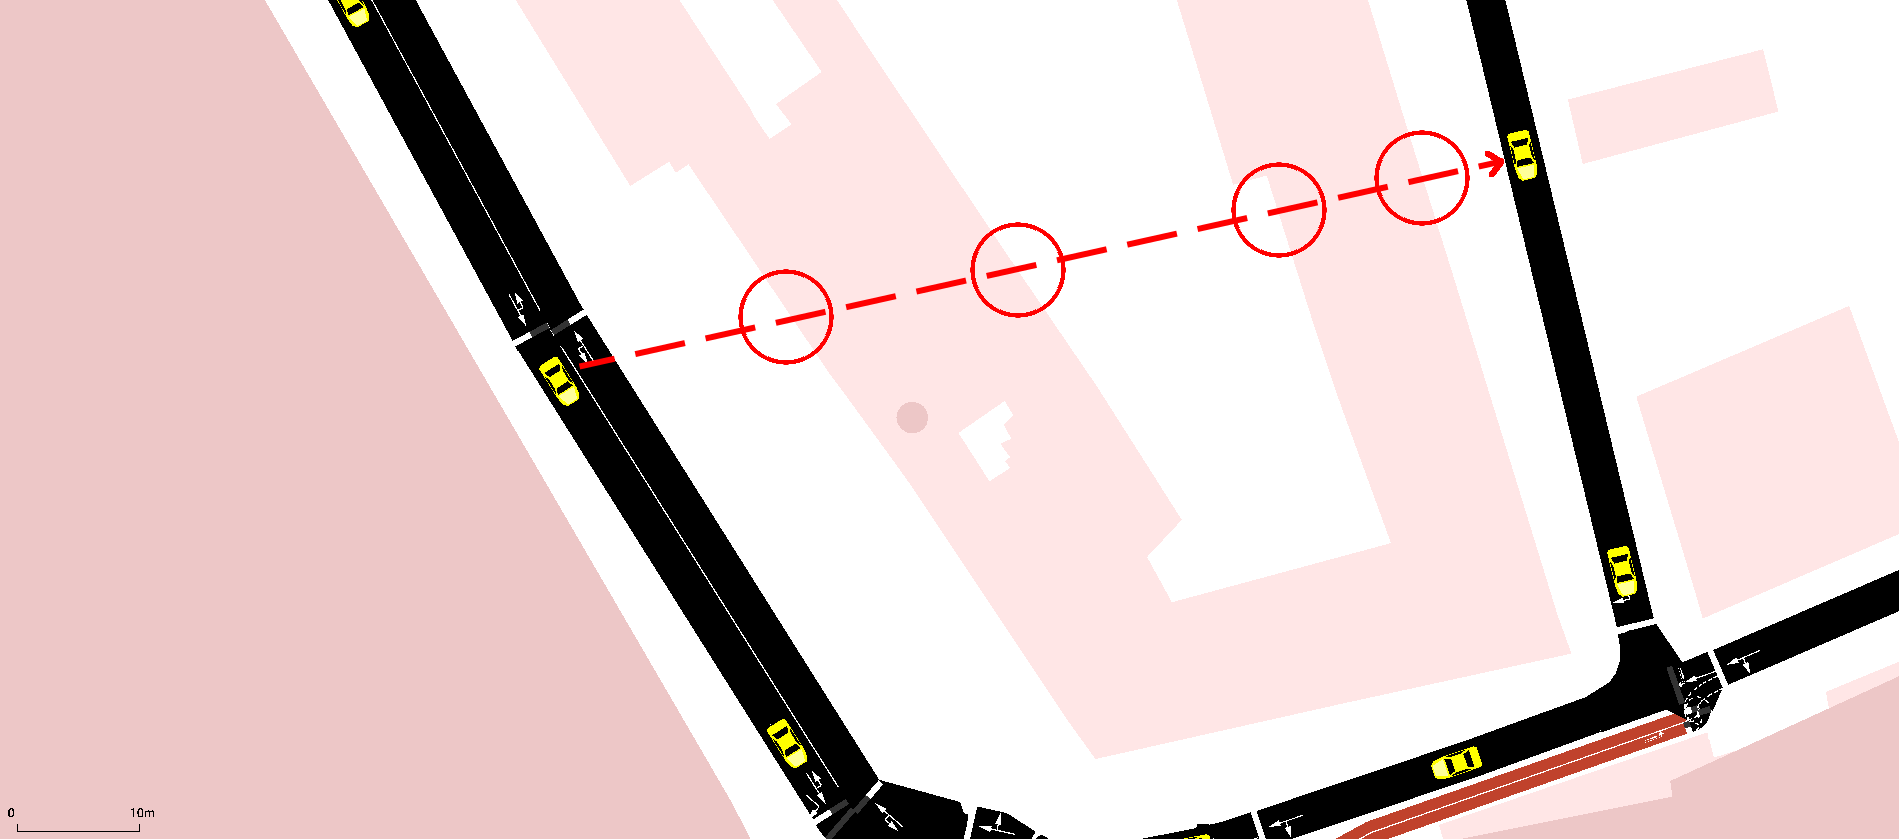
\includegraphics[width=\textwidth]{immagini/sumo-obstacle}
			\caption{Example of obstacle shadowing in vehicle-to-vehicle communication. Walls encountered by the signal are surrounded in red circles}
			\label{fig:sumo-obstacle}
		\end{figure}
	
	\section{Emergency Message Dissemination and broadcasting protocols}
		\label{sec:emd}
		Emergency Message Dissemination (EMD) is a fundamental application in \acrshort{vaneta} to prevent traffic accidents, thereby reducing death and injury rates. Such task can be execute by the VANET itself by turning it into an infrastructure-less self-organizing network, where the dissemination is carried out by specific protocols. 
		
		
		Since the traffic information, especially the emergency data, has a broadcast-oriented nature (i.e. it is of public interest), it is more appropriate to disseminate it using broadcasting routing scheme rather than unicast or multicast ones. \cite{5989903}
%		suddivisione broadcasting protocols
		
		This choice leads to some advantages, such as:
		\begin{itemize}
			\item the fact that vehicles do not need to know the destination address and how to calculate a route towards it;
			\item a greater coverage of vehicles interested in the information, useful also in lossy scenarios, especially when paired with controlled redundancy schemes;
			\item a greater efficiency in bandwidth usage.
		\end{itemize}
		
		The idea behind existing algorithms consists in designating the next forwarder in the multi-hop chain from the source of the alert to the target region where the sensitive data has to be delivered. Ideally, the farthest vehicle from a previous forwarder in the dissemination direction should be given priority when designating the next forwarder. However, due to unreliable wireless channel the designation of farthest vehicle can fail and interrupt the message dissemination. Due to this, next forwarder designation keeps into consideration vehicles (called potential forwarder candidates, PFCs) which have received an Alert Message. The PFCs participate in contention to elect the farthest forwarder candidate (FFC) who will continue disseminating the message.
		
		
		In order to carry out the forwarder designation process, the main idea consists in differentiating waiting times (WT) of PFCs. Each PFC should select a waiting time ranging from 0 to a predefined upper bound (PUB). To guarantee the correct designation of the farthest vehicle as forwarder, PFCs choose their waiting time inversely proportional to the distance between the PFC and the previous forwarder. This way other candidates can detect the transmission from the FFC and suppress their transmission.
		
		Advancements in research on Emergency Message Dissemination has lead to the development of a number of broadcasting protocols. However, as identified by Panichpapiboon et al.\cite{5989903}, most of them belong to one of two main categories:
		\begin{itemize}
			\item Multi-hop Broadcasting Protocols, in which packets are transmitted through the network via flooding by some of the neighbors of the source. It is of utmost importance to reduce the number of redundant transmission in order not to waste bandwidth.
			\item Single-hop Broadcasting Protocols, in which no flooding is employed. Instead, vehicles periodically select and broadcast only a subset of the packets it has received.
		\end{itemize}
		
		
		Multi-hop Broadcasting Protocols can be further subdivided into two categories:
		\begin{enumerate}
			\item Delay based protocols, which assign a different waiting time before rebroadcasting the message to each vehicle. This delay is usually inversely proportional to the distance between the source and the potential sender.
			Some examples are:
			\begin{itemize}
				\renewcommand\labelitemi{--}
				\item \textit{Urban Multi-hop Broadcast (UMB)} \cite{Korkmaz:2004:UMB:1023875.1023887}, designed to solve the broadcast redundancy, hidden node and reliability problems in multi-hop broadcasting using \textit{Request-to-Broadcast (RTB)} and \textit{Clear-To-Broadcast (CTB)} packets; 
				\item \textit{Smart Broadcast (SB)} \cite{4025102} and \textit{Efficient Directional Broadcast (EDB)} \cite{4340158}, which try to reduce the delay introduced by UMB and remove the RTB and CTB packets, respectively;
				\item \textit{Vehicle-density-based Emergency Broadcasting (VDEB)} \cite{5663803}, a slotted broadcasting protocol which keeps vehicle density into consideration when computing waiting time slots;
				\item \textit{Reliable Method for Disseminating Safety Information
				(RMDSI)} \cite{4591259}, which aims to offer better performances when the network becomes fragmented by making a forwarder keep a copy of the packet it has broadcasted until it hears a retransmission (or until the packet lifetime expires). If no retransmission is heard within a certain time limit, the forwarder tries to find the next node which can relay the message using a small control packet;
				\item \textit{Multi-hop Vehicular Broadcast (MHVB)} \cite{4068699}, a protocol that keeps traffic congestion into consideration by   checking whether the number of neighbors of a vehicle is greather than a certain threshold and its speed is less than another threshold. When a node detects congestion, it increases its broadcast interval in order to try to reduce the network load;
				\item \textit{Reliable Broadcasting of Life Safety Messages (RBLSM)} \cite{4458046}, whose main objective is reliability, and a higher priority is given to the vehicle nearest to the sender instead to the one furthest from it, due to the assumption that the closer the vehicle is, the more reliable it is considered since its received signal strength is higher.
			\end{itemize}
		
			\item Probabilistic-based Multi-hop Broadcasting Protocols
			The idea behind these kind of protocols is similar to the one behind Delay based protocols, but instead of assigning a different rebroadcast delay to each vehicle, a different rebroadcast probability is assigned. Each protocol differs in the function that assigns probabilities. Some examples of probabilistic-based protocols are:
			\begin{itemize}
				\renewcommand\labelitemi{--}
		 		\item \textit{Weighted p-Persistence} \cite{4407231}, in which every PFC computes its own rebroadcast probability based on distance between itself and the transmitter. The formula used is the following:
				\begin{gather}
		 			p_{ij} = \frac{D_{ij}}{R}
		 			\label{eq:weighted-p-persistence}
 				\end{gather}
 				where $D_{ij}$ is the distance between transmitter \textit{i} and PFC \textit{j} and R is the transmission range. Given this function, the probability to rebroadcast is proportional to the distance between the PFC and the transmitter. The abovementioned formula does not keep into account vehicle density and also assumes that the transmission range is fixed and known to all vehicles.
 				
 				\item \textit{Optimized Adaptive Probabilistic Broadcast (OAPB)\cite{1543865} and AutoCast (AC) \cite{4350058}}, which both keep the vehicle density into consideration when computing the forwarding probability by making vehicle periodically exchange Hello messages. Thanks to those messages, each vehicle can compute the number of neighbors and then use this information accordingly.
 				
 				\item \textit{Irresponsible Forwarding (IF)} \cite{4740277}\cite{5426212}, a protocol that considers vehicle density like OAPB and AC, but the formula used is not a simple linear function. In fact, the rebroadcast probability assignment function is the following:
 				\begin{gather}
 					p = e^{-\frac{\rho_s(z-d)}{c}}
 				\end{gather}
 				where $\rho_s$ is the vehicle density, $z$ is the transmission range, $d$ is the distance between the PFC and the transmitter and $c\geq1$ is a shaping parameter which influences rebroadcast probability. Irresponsible Forwarding aims to offer a solution that can scale with network density.
			\end{itemize}
		
%		\item Network Coding-Based Multi-hop Broadcasting. TODO? da fare?
		
		Vehicles employing Single-Hop Broadcasting protocols will not flood received packets immediately through the network. Instead, vehicles use information from packets to update their database and periodically rebroadcast only a fraction of that information. The two variables these kind of protocol can work on to aim for good network efficiency are:
		\begin{itemize}
			\item \textit{Broadcast Interval}, i.e. the amount of time between retransmissions, which should keep into consideration both freshness of information and potential redundancy in transmissions;
			\item \textit{Relevancy of information} to broadcast: as stated before, only relevant information (i.e. a subset of all the information) should be broadcast.
		\end{itemize}
		
		Single-Hop protocols can be further subdivided into two categories:
		\begin{enumerate}
			
			\item Fixed Broadcast Interval, which keep the Broadcast Interval fixed. Some exampels are:
			\begin{itemize}
				\renewcommand\labelitemi{--}
				
				\item \textit{TrafficInfo}\cite{4621303}, a protocol in which vehicles record, among other information, travel times on road segments (identified by an ID) and keep them on its on-board database. Vehicles periodically exchange information about the learned travel times based on the relevance of such information. The relevance is calculated using a ranking algorithm which uses the current position of the vehicle and the current time (i.e. relevance decreases with distance and time), broadcasting only the $k$  most important information. 
				
				\item \textit{TrafficView}\cite{1263039}, in which vehicles exchange information about speed and position and record it in their database. Data about different vehicles is then aggregated into a single record using one of two aggregation algorithms:
				\begin{itemize}
					\item the \textit{ratio-based} algorithm, which assigns an aggregation ratio to each portion of a road: the more important the road is, the higher the aggregation ratio will be, increasing the accuracy of the information of that area.
					\item the \textit{cost-based} algorithm, an algorithm which keeps into consideration the cost of aggregating different records. The aggregation cost is defined as the loss of accuracy the aggregation will bring about.
				\end{itemize} 
			\end{itemize}
			\item Adaptive Broadcast Interval, which adapt the Broadcast Interval based on dynamic information. Some examples are:
			\begin{itemize}
				\renewcommand\labelitemi{--}
				
				\item \textit{Collision Ratio Control Protocol (CRCP)}\cite{4357748}, a scheme according to which vehicles exchange information about location, speed and road ID. The Broadcast Interval is dynamically controlled based on the amount of detected collisions and bandwidth efficiency: the protocol tries to maintain the number of collisions under a certain threshold by doubling the Broadcast Interval every time the threshold is exceeded. Otherwise, the Broadcast Interval is decreased by one second when the bandwidth efficiency decreases too much.
				
				Moreover, the authors propose three different methods for selecting the data to be transmitted:
				\begin{itemize}
					\item \textit{Random Selection}: a vehicle selects a random information in its database and broadcasts it;
					\item \textit{Vicinity Priority Selection}: vehicles give priority to information of nearby areas;
					\item \textit{Vicinity Priority Selection with Queries}: similar to Vicinity Priority Selection, with the possibility of querying information for a certain area.
				\end{itemize}
				
				\item \textit{Abiding Geocast:}\cite{4531929}, which aims to deliver an Alert Message to a specific area where the warning is still relevant. Only vehicles that are travelling towards the effective area can participate in contention to broadcast the message. Moreover, broadcast is dynamically adjusted based on transmission range, speed, and distance between the potential forwarder and the destination area, increasing when such distance increases or the potential forwarder's speed decreases.
				
				\item \textit{Segment-oriented Data Abstraction and Dissemination
					(SODAD)}\cite{1402433}, a protocol according to which roads are divided into segments and each vehicle can both discover information itself and collect it from neighbor's transmissions. Whenever a vehicle receives a transmission from another vehicle, the information received will be classified as either one of two events:
					\begin{itemize}
						\item a \textit{provocation} event that will decrease the Broadcast Interval;
						\item a \textit{mollification} event that will increase the Broadcast Interval.
					\end{itemize}
					The classification is done via comparison of the newly received data with the information stored in the vehicle's on-board database. The vehicle assigns a higher weight if the difference between information coming from these two sources is high. The weight will be then compared against a threshold to establish whether a provocation of mollification event has taken place.
			\end{itemize}
		
		The authors of ROFF \cite{6906275}, a Multi-Hop delay based protocol, state that existing protocols are affected by two problems:
		\begin{itemize}
			\item the perfect suppression of redundant transmissions, by which potential forwarders which have lost the contention detect the transmission from the farthest vehicle and suppress their transmission. However this suppression can not always be guaranteed due to short difference between waiting times. In fact, if the timer of a potential forwarder expires before it has heard the transmission from the FFC, a redundant transmission will occur;
			\item the disuniformity and the costant change in spatial vehicle distribution in VANETs. Existing protocols which keep into consideration the distance between PFC and previous forwarder do not keep into consideration large empty spaces in the waiting time computation, leading to unnecessary wait.
		\end{itemize}
		ROFF's solutions to these problems and the implementation of the protocol will be analyzed in Chapter \ref{chapter:roff}
		
%		The previous thesis \cite{ROM2017} focused on the evaluation of Fast Broadcast \cite{4199282}, a Multi-Hop delay based protocol, through simulation in various scenarios. 
			
		\end{enumerate}
		
		\end{enumerate}  
% !TEX encoding = UTF-8
% !TEX TS-program = pdflatex
% !TEX root = ../tesi.tex

\chapter{Models}	
	In this Chapter the models implemented and utilized in this work will be presented, namely the Obstacle Shadowing propagation loss model (Section \ref{sec:shadowing}) and the Junction model (Section \ref{sec:junction-modeling}).
	
	\section{Obstacle Shadowing propagation loss model}
		\label{sec:shadowing}
		The original thesis \cite{ROM2017}, after having analyzed various works concerning shadowing in urban scenarios \cite{Giordano:2010:CST:1860058.1860065} \cite{4020783}, used a deterministic \gls{rpma} called Obstacle Shadowing propagation loss model presented in \cite{5720204} and implemented by the authors of \cite{Carpenter:2015:OMI:2756509.2756512}.  This propagation model calculates the loss in signal strength due to the shadowing effect of obstacles such as buildings. 
		
		
		The authors of \cite{5720204} designed the model as an extension of well-established fading models, which can be expressed by Equation \ref{eq:fading-models}, where:
		\begin{itemize}
			\item $P$ are the transmit or receive powers of the radios;
			\item $G$ are the antenna gains;
			\item $L$ indicate the terms capturing loss effects during transmission.
		\end{itemize}
		
		\begin{gather}
			P_r[dBm] = P_t[dBm] + G_t[dB] + G_r[dB] - \sum L_x[dB] 														\label{eq:fading-models}
		\end{gather}
	
		Common RPMs can be written as components L of \ref{eq:fading-models} and chained to obtain the compound attenuation. For example, Equation \ref{eq:tworayground-model} and \ref{eq:lognorm-model} represent respectively the Two-Ray Ground and Log-Normal models.

		\begin{gather}
			L_{TwoRayGround} = 10 \lg \left( \frac{d^4 L}{h^2_t h^2_t} \right)	\qquad [dB]		\label{eq:tworayground-model} \\
			L_{LogNorm} = 10 \lg \left( X_\sigma \right)	\qquad [dB]													\label{eq:lognorm-model}
		\end{gather}
		
		The authors extended the general model shown in \ref{eq:fading-models} adding a $L_{obs}$ term for each obstacle in the line of sight between sender and receiver. The term is described by Equation \ref{eq:osbtacle-model}, where:
		\begin{itemize}
			\item $n$ is the number of times that the line of sight intersects the borders of the obstacle;
			\item $d_m$ is the length of the obstacle's intersections;
			\item $\beta$ represents the attenuation due to the exterior wall of a building, in dB per wall;
			\item $\gamma$ represents an approximation of the internal structure of a building, in dB per meter.
		\end{itemize}
		
		
		Parameters $\beta$ and $\gamma$ can be fitted to represent different types of buildings. $\beta \approx$ 9.6 dB per wall and $\gamma \approx$ 0.4 dB/m are the values proposed by the authors for buildings in suburban areas.
		
		\begin{gather}\label{eq:osbtacle-model}
			L_{obs} = \beta n + \gamma d_m
		\end{gather}
	
		\imgrefcap{fig:sumo-obstacle} shows an example of transmission where the signal encounters $n =$ 4 walls. 
	
		\begin{figure}[H]
			\centering
			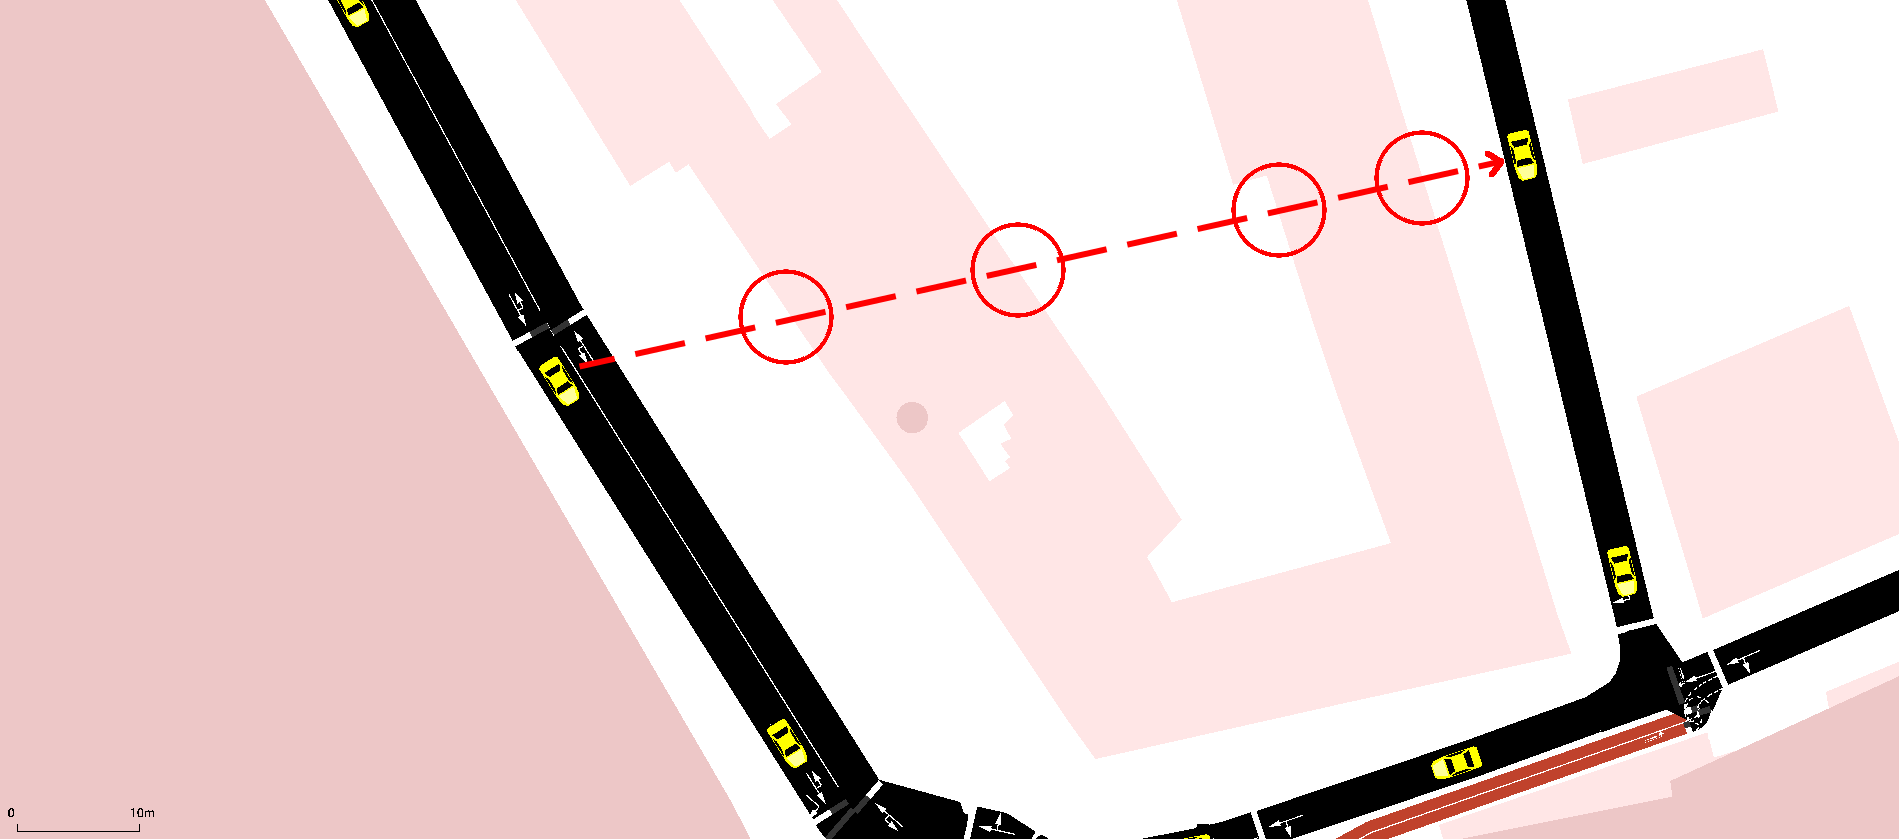
\includegraphics[width=\textwidth]{immagini/sumo-obstacle}
			\caption{Example of obstacle shadowing in vehicle-to-vehicle communication. Walls encountered by the signal are surrounded in red circles}
			\label{fig:sumo-obstacle}
		\end{figure}
	
	\section{Junction modeling}
		\label{sec:junction-modeling}
		Part of this work consisted in implementing extensions for the algorithms which will be presented in Chapter \ref{chapter:fb} and \ref{chapter:roff} to utilize road junctions in a smart way. These extensions aim to reach a higher number of vehicles during the Alert Message propagation. In order for those extension to work, a model to identify and represent junctions was necessary. Using data retrieved from OpenStreetMap elaborated through SUMO (see Section \ref{sec:sumo} for the full process), it has been possible to retrieve information about junctions present inside a urban scenario. Figure \ref{fig:junction} shows the JSON representation of a junction.
		
		\begin{figure}[H]
			\centering
			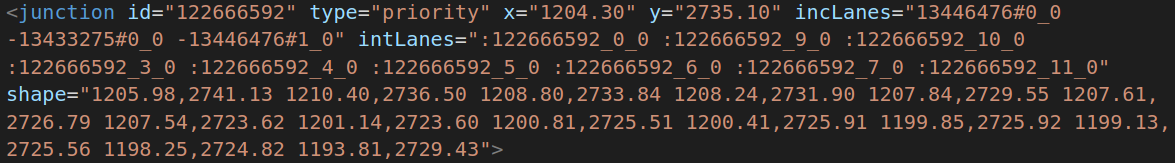
\includegraphics[width=\textwidth]{immagini/junction}
			\caption{Example of data about a junction retrieved from OpenStreetMap and elaborated through SUMO}
			\label{fig:junction}
		\end{figure}
		
		Among other data, the most useful information about a junction are:
		\begin{itemize}
			\item the \textit{x} and \textit{y} coordinates, which identify its center;
			\item the \textit{shape} attribute, containing coordinates which represent its shape.
		\end{itemize}
		
		Using from this data it was possible to establish the junction modeling process, represented in Figure \ref{fig:junction-process}. Since the \textit{shape} attribute resulted in a polygon too small for the purpose of this work, a bounding box which extends the polygon by 20 meters in each direction has been implemented.
		
		\begin{figure}[H]
			\centering
			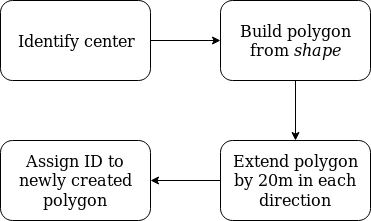
\includegraphics[width=0.4\textwidth]{immagini/junction-process}
			\caption{Junction modeling process}
			\label{fig:junction-process}
		\end{figure}
	
		Figure \ref{fig:junction-example} shows the results of the above-mentioned process executed on six different junctions. The red polygon is the polygon defined by the \textit{shape} attribute in the JSON definition of a junction, while the yellow rectangle is the bounding box. Each vehicle knows whether it is inside a junction based on its coordinates. A vehicle is inside a junction only if its coordinates are inside of one of the bounding boxes.
	
		\begin{figure}[H]
			\centering
			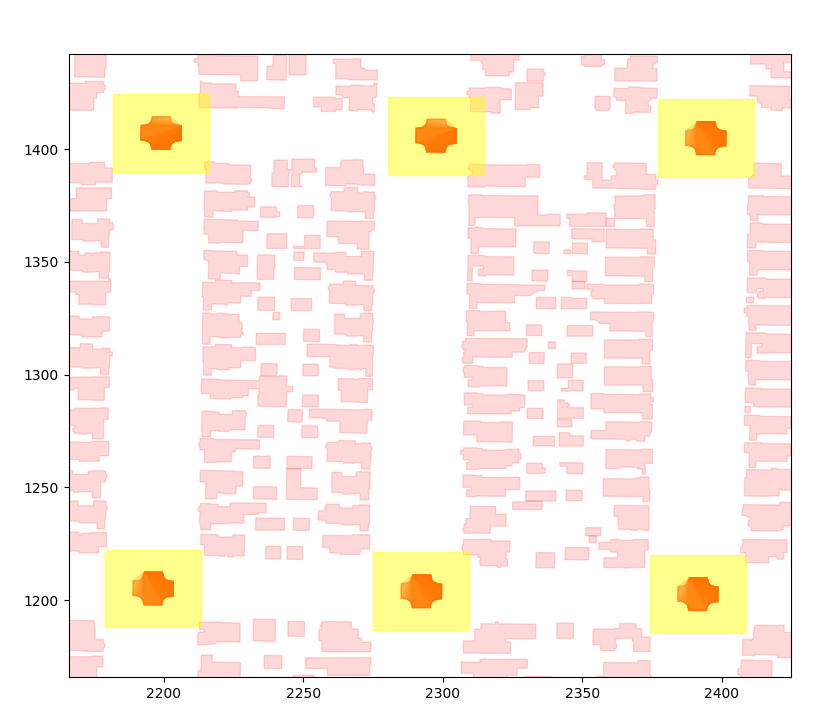
\includegraphics[width=0.48\textwidth]{immagini/junction-example}
			\caption{Example of 6 junctions in an urban scenario}
			\label{fig:junction-example}
		\end{figure}
		  
% !TEX encoding = UTF-8
% !TEX TS-program = pdflatex
% !TEX root = ../tesi.tex

\chapter{Fast-Broadcast}
	\label{chapter:fb}
	Fast-Broadcast \cite{4199282} is a multi-hop routing protocol for vehicular communication. Its main feature consists in breaking the assumption that all vehicles should know, \textit{a priori}, their fixed and constant transmission range. This assumption is often unreasonable, especially in \acrshort{vaneta}s and urban environments, where electromagnetic interferences and obstacles such as buildings heavily influence the transmission range.
	
	
	Fast-Broadcast employs two different phases:
	\begin{enumerate}
		\item the \textbf{Estimation Phase}, during which vehicles estimate their frontward and backward transmission range;
		\item the \textbf{Broadcast Phase}, during which a vehicle sends an Alert Message and the other cars need to forward it in order to propagate the information.
	\end{enumerate}

	\section{Estimation Phase}
		During this phase, vehicles try to estimate their frontward and backward transmission range by the means of Hello Messages. These beacons are sent periodically via broadcast to all the neighbors of a vehicle.
		
		
		Time is divided into turns and, in order to keep estimations fresh, data collected during a certain turn is kept for the duration of the next turn, then discarded. The parameter \textit{turnSize} specifies the duration of a turn: the authors suggest a duration of one second. A bigger \textit{turnSize} could guarantee less collisions to the detriment of freshness of information. On the other hand, the effects of a smaller \textit{turnSize} are specular to those just presented. 
		
		
		Using this approach, vehicles can estimate two different values:
		\begin{itemize}
			\item \textit{Current-turn Maximum Front Range (\textit{CMFR})}, which estimates the maximum frontward distance from which another car can be heard by the considered one;
			\item \textit{Current-turn Maximum Back Range} (\textit{CMBR}), which estimates the maximum backward distance at which the considered car can be heard.
		\end{itemize}
		When the turn expires, the value of these variables is stored in the \textit{LMFR} and \textit{LMBR} variables (\textit{Latest-turn Maximum Front Range} and \textit{Latest-turn Maximum Back Range}, respectively). The algorithm uses both last turn and current turn data because the former guarantees values calculated with a larger pool of Hello Messages, while the latter considers fresher information.
		
		When sending a Hello Message (Algorithm \ref{alg:hello-message-sending-1d}), the vehicle initially waits for a random time between 0 and \textit{turnSize}. After this, if it has not heard another Hello Message or a collision, it proceeds to transmit a Hello Message containing the estimation of its frontward transmission range.
		
		
		When receiving a Hello Message (Algorithm \ref{alg:hello-message-receiving-1d}), the vehicle retrieves its position and the sender's position, calculates the distance between these two positions and then updates the \textit{CMFR} field if the message comes from ahead, otherwise \textit{CMBR} is updated. The new value is obtained as the maximum between the old \textit{CMFR} or \textit{CMBR} value, the distance between the vehicle and the sender, and the sender's transmission range estimation included in the Hello Message.
		
		\begin{algorithm}[H]
			\begin{algorithmic}[1]
				\ForEach{turn}
					\State sendingTime $\gets$ random(turnSize)
					\State wait(sendingTime)
					\If{$\neg$ (heardHelloMsg() $\lor$ heardCollision())}
						\State helloMsg.declaredMaxRange $\gets$ max(LMFR, CMFR)
						\State helloMsg.senderPosition $\gets$ retrievePosition()
						\State transmit(helloMsg)
					\EndIf
				\EndFor
			\end{algorithmic}
			\caption{Hello message sending procedure for 1D}
			\label{alg:hello-message-sending-1d}
		\end{algorithm}
		
		\begin{algorithm}[H]
			\begin{algorithmic}[1]
				\State myPosition $\gets$ retrievePosition()
				\State senderPosition $\gets$ helloMsg.senderPosition
				\State declaredMaxRange $\gets$ helloMsg.declaredMaxRange
				\State d $\gets$ distance(myPosition, senderPosition)
				\If{receivedFromFront(helloMsg)} 
				\State CMFR $\gets$ max(CMFR, d, declaredMaxRange)
				\Else
				\State CMBR $\gets$ max(CMBR, d, declaredMaxRange)
				\EndIf
			\end{algorithmic}
			\caption{Hello message receiving procedure for 1D}
			\label{alg:hello-message-receiving-1d}
		\end{algorithm}
	
	\section{Broadcast Phase}
		This phase is activated once a vehicle sends an Alert Message. The other cars can exploit the estimation of transmission ranges to reduce redundancy in message broadcast. Each vehicle can exploit this information to assign itself a forwarding priority inversely proportional to the relative distance: the higher the relative distance, the higher the priority.  
		
		
		When the Broadcast Phase is activated, a vehicle sends an Alert Message with application specific data. Broadcast specific data is also piggybacked on the Alert Message, such as:
		\begin{itemize}
			\item \textit{MaxRange:} the maximum range a transmission is expected to travel backward before the signal becomes too weak to be received. This value is utilized by following vehicles to rank their forwarding priority;
			\item \textit{SenderPosition}: the coordinates of the sender.
		\end{itemize}
		Upon reception, each vehicle waits for a random time called \textit{Contention Window} (\textit{CW}). This window ranges from a minimum value (\textit{CWMin}) and a maximum one (\textit{CWMax}) depending on sending/forwarding car distance (\textit{Distance}) and on the estimated transmission range (\textit{MaxRange}), according to formula \ref{eq:contention-window}. It is quite easy to see that the higher the sender/forwarder distance is, the lower the contention window is.
		\begin{gather}
			\left\lfloor \left( \frac{\text{MaxRange} - \text{Distance}}{\text{MaxRange}} \times (\text{CWMax} - \text{CWMin}) \right) + \text{CWmin}  \right\rfloor
			\label{eq:contention-window}
		\end{gather}
		If another forwarding of the same message coming from behind is heard during waiting time, the vehicle suppresses its transmission because the message has already been forwarded by another vehicle farther back in the column. On the contrary, if the same message is heard coming from the front, the procedure is restarted using the new parameters. The vehicle can forward the message only if the waiting time expires without having received the same message.
		
		Algorithm \ref{alg:alert-message-generation-1d} and \ref{alg:alert-message-forwarding-1d} describe the logic behind the Broadcast Phase.
		
		\begin{algorithm}[H]
			\begin{algorithmic}[1]
				\State alertMsg.maxRange $\gets$ max(LMBR, CMBR)
				\State alertMsg.position $\gets$ retrievePosition()
				\State transmit(alertMsg)
			\end{algorithmic}
			\caption{Alert Message generation procedure for 1D}
			\label{alg:alert-message-generation-1d}
		\end{algorithm}
	
		\begin{algorithm}[H]
			\begin{algorithmic}[1]
				\State cwnd $\gets$ computeCwnd()
				\State waitTime $\gets$ random(cwnd)
				\State wait(waitTime)
				\If{sameBroadcastHeardFromBack()}
				\State exit()
				\ElsIf{sameBroadcastHeardFromFront()}
				\State restartBroadcastProcedure()
				\Else 
				\State alertMsg.maxRange $\gets$ max(LMBR, CMBR)
				\State alertMsg.senderPosition $\gets$ retrievePosition()
				\State transmit(alertMsg)
				\EndIf 
			\end{algorithmic}
			\caption{Alert Message forwarding procedure for 1D}
			\label{alg:alert-message-forwarding-1d}
		\end{algorithm}
	
	\section{Multiple dimensions extension}
		\label{sec:fb-multiple-dimensions}
		The original work \cite{4199282} considered only a strip-shaped road, where it was easy to define directions and establish when a message came from the front or the back. In \cite{BAR2017} an extension considering two dimensions was proposed. This work proposes a modification to that version, since it caused some delivery problems in particular scenarios. This section will firstly present the original extension of \cite{BAR2017} and then discuss the proposed modification.
		
		
		The modifications to the Fast-Broadcast algorithm are the following:
		\begin{enumerate}
			\item Utilizing only one parameter between \textit{CMBR} and \textit{CMFR} (thus considering only \textit{CMR}):
			\item including the position of the vehicle which originally generated the Alert Message in addition to the position of the sender of the message.
		\end{enumerate}
		
		
		As explained in the original extension, when a vehicle receives an Alert Message, the origin-vehicle distance is confronted with the origin-sender distance: the vehicle can forward the message only if the former is greater than or equal to the latter, otherwise it simply discards the message.
		
		\begin{figure}[H]
			\centering
			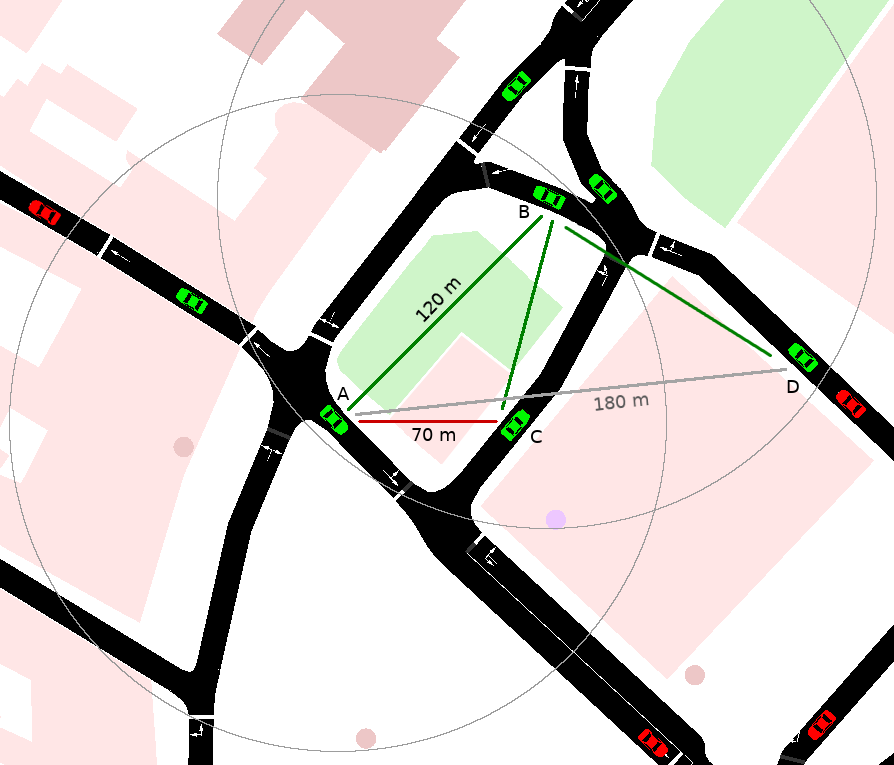
\includegraphics[width=\textwidth]{immagini/fb-2dpicc}
			\caption{Example of Fast-Broadcast in 2D scenario}
			\label{fig:fb-2d}
		\end{figure}
		
		
		
		For example, suppose that vehicle A is the origin of the Alert Message and B receives it, but C doesn't due to an obstacle in the line of sight. B computes origin-vehicle distance, $d(A, B)$, and origin-sender distance, $d(A, A)$, which in this case are respectively 120 and 0m. Since origin-vehicle is greater than origin-sender, B can forward the Alert Message.
		
		
		Now suppose that C receives the message from B. C computes origin-vehicle distance, $d(A, C)$, and origin-sender distance, $d(A, B)$, which amount to 70 and 120m respectively. Since the former is not greater than or equal to the latter, C is not a candidate for forwarding and suppresses the transmission.
		
		
		D receives the message from B as well. D is a good candidate for transmission since the origin-vehicle distance, which amounts to 180m, is greater than origin-sender distance, equal to 120m.
		
		However, the condition by which vehicles suppressed their transmission when the origin-sender distance was smaller than the origin-sender distance causes delivery problems in particular scenarios, reported in Appendix \ref{chapter:fbmod}. Hence, that condition has been dropped in the algorithm implemented in this work. Referring to the example in Figure \ref{fig:fb-2d}, this change makes vehicle C a forwarder candidate as well.
		
		Algorithm \ref{alg:hello-message-sending-2d}, \ref{alg:hello-message-receiving-2d}, \ref{alg:alert-message-generation-2d} and \ref{alg:alert-message-forwarding-2d} show the implementation for Fast-Broadcast for multiple dimensions (mainly 2D, but this version actually works also for 3D scenarios, for example scenarios with only drones or with drones and vehicles).
		
		\begin{algorithm}[H]
			\begin{algorithmic}[1]
				\ForEach{turn}
				\State sendingTime $\gets$ random(turnSize)
				\State wait(sendingTime)
				\If{$\neg$ (heardHelloMsg() $\lor$ heardCollision())}
				\State helloMsg.declaredMaxRange $\gets$ max(LMR, CMR)
				\State helloMsg.senderPosition $\gets$ retrievePosition()
				\State transmit(helloMsg)
				\EndIf
				\EndFor
			\end{algorithmic}
			\caption{Hello message sending procedure for 2D}
			\label{alg:hello-message-sending-2d}
		\end{algorithm}
		
		\begin{algorithm}[H]
			\begin{algorithmic}[1]
				\State myPosition $\gets$ retrievePosition()
				\State senderPosition $\gets$ helloMsg.senderPosition
				\State declaredMaxRange $\gets$ helloMsg.declaredMaxRange
				\State d $\gets$ distance(myPosition, senderPosition)
				\State CMR $\gets$ max(CMR, d, declaredMaxRange)
			\end{algorithmic}
			\caption{Hello message receiving procedure for 2D}
			\label{alg:hello-message-receiving-2d}
		\end{algorithm}
	
	
		\begin{algorithm}[H]
			\begin{algorithmic}[1]
				\State alertMsg.maxRange $\gets$ max(LMR, CMR)
				\State alertMsg.senderPosition $\gets$ retrievePosition()
				\State alertMsg.originPosition $\gets$ retrievePosition()
				\State transmit(alertMsg)
			\end{algorithmic}
			\caption{Alert Message generation procedure for 2D}
			\label{alg:alert-message-generation-2d}
		\end{algorithm}
	
		\begin{algorithm}[H]
			\begin{algorithmic}[1]
				\State cwnd $\gets$ computeCwnd()
				\State waitTime $\gets$ random(cwnd)
				\State wait(waitTime)
				\If{sameBroadcastHeardFromBack()}
				\State exit()
				\ElsIf{sameBroadcastHeardFromFront()}
				\State restartBroadcastProcedure()
				\Else 
				\State alertMsg.maxRange $\gets$ max(LMR, CMR)
				\State alertMsg.senderPosition $\gets$ retrievePosition()
				\State transmit(alertMsg)
				\EndIf 
			\end{algorithmic}
			\caption{Alert Message forwarding procedure for 2D}
			\label{alg:alert-message-forwarding-2d}
		\end{algorithm}
	
		\subsection{Hello Message Header Structure}
			The Hello Message header structure is represented in Figure \ref{fig:fbHelloHeader}.
			\begin{figure}[H]
				\centering
				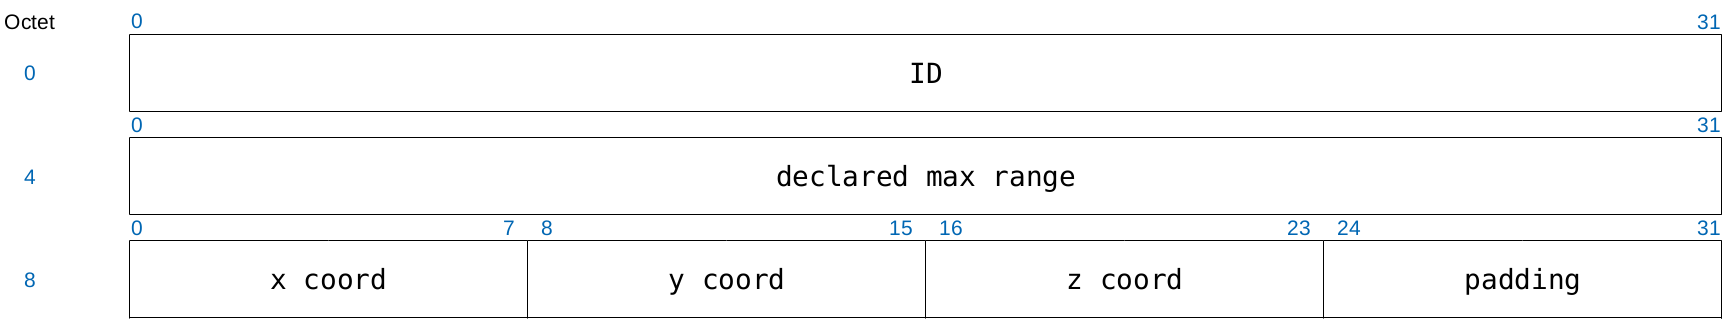
\includegraphics[width=\textwidth]{immagini/fbHelloHeader}
				\caption{Fast-Broadcast Hello Message header structure}
				\label{fig:fbHelloHeader}
			\end{figure}
			
			The fields contained in the Hello Message are the following:
			\begin{itemize}
				\item \textit{ID}: unique ID of the Hello Message's sender;
				\item \textit{declared max range}: maximum range detected by the vehicle during Estimation Phase;
				\item \textit{x coord}, \textit{y coord} and \textit{z coord}: coordinates of the Hello Message's sender.
			\end{itemize}
		
		\subsection{Alert Message Header Structure}
			The Alert Message header structure is represented in Figure \ref{fig:fbAlertHeader}.
			\begin{figure}[H]
				\centering
				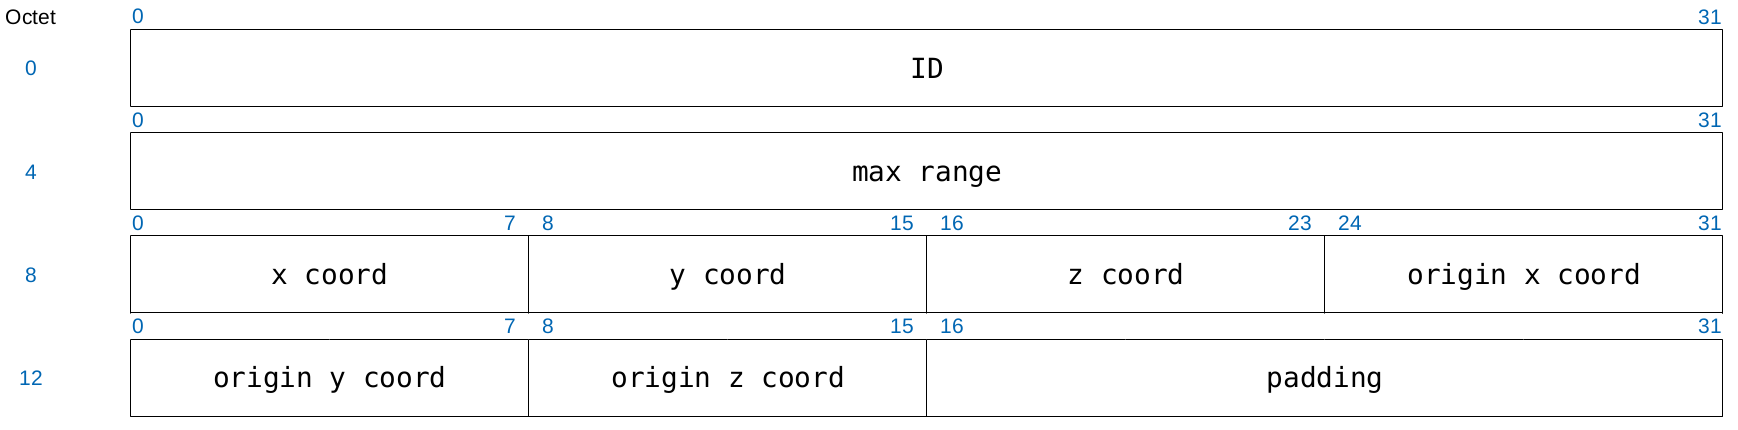
\includegraphics[width=\textwidth]{immagini/fbAlertHeader}
				\caption{Fast-Broadcast Alert Message header structure}
				\label{fig:fbAlertHeader}
			\end{figure}
		
		The fields contained in the Alert Message are the following:
		\begin{itemize}
			\item \textit{ID}: unique ID of the Alert Message's sender;
			\item \textit{max range}: maximum range detected by the vehicle during Estimation Phase;
			\item \textit{x coord}, \textit{y coord} and \textit{z coord}: coordinates of the Hello Message's sender;
			\item \textit{origin x}, \textit{origin y} and \textit{origin z coord}: coordinates where the Alert initially originated from.
		\end{itemize}
	
	\section{Smart Junction Fast-Broadcast (SJ-Fast-Broadcast)}
		\label{sj:fb}
		This work proposes an extension for Fast-Broadcast which keeps junctions into consideration in order to achieve a greater delivery ratio of Alert Messages. The idea comes from the following observation: whenever buildings block signal propagation across different roads, the message is relayed only through the road segments inside the forwarder's field of view. This causes the Alert Message propagation to spread:
		\begin{itemize}
			\item in one direction, if the forwarder is not inside a junction and the road segment is surrounded by buildings which block the signal;
			\item in three directions, whenever the forwarder lies inside a junction. 
		\end{itemize}
		Actually the signal travels respectively in two and four directions, but we are not considering the direction where the previous Alert Message is coming from (i.e. we are only considering forwarding towards previously uncovered areas in this analysis).
		Referring to Figure \ref{fig:fb-junction-0}, if the message is coming from the top and A and B forwards it, then only vehicles in the north-south road will be reached. Vehicles on the west-east road will be reached by the Alert Message at a later point, if the propagation circles back to them through another road, otherwise they will never be informed about the alert. If C is also forced to forward, then we have coverage across all road segments and the propagation can continue towards all directions. Figure \ref{fig:fb-junction-1} shows an example where SJ-Fast-Broadcast is employed and a greater coverage is achieved.
		
		\begin{figure}[H]
			\centering
			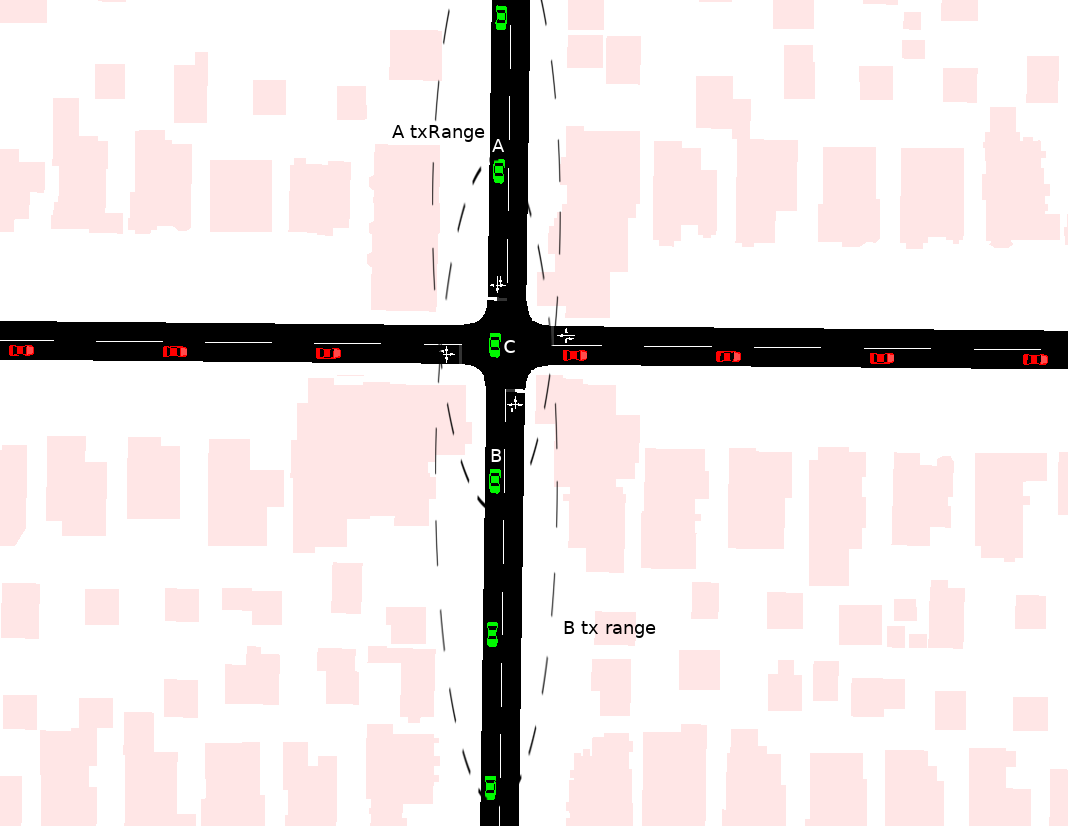
\includegraphics[width=\textwidth]{immagini/fb-junction-0}
			\caption{Usual Fast-Broadcast Alert Message propagation}
			\label{fig:fb-junction-0}
		\end{figure}
	
		\begin{figure}[H]
			\centering
			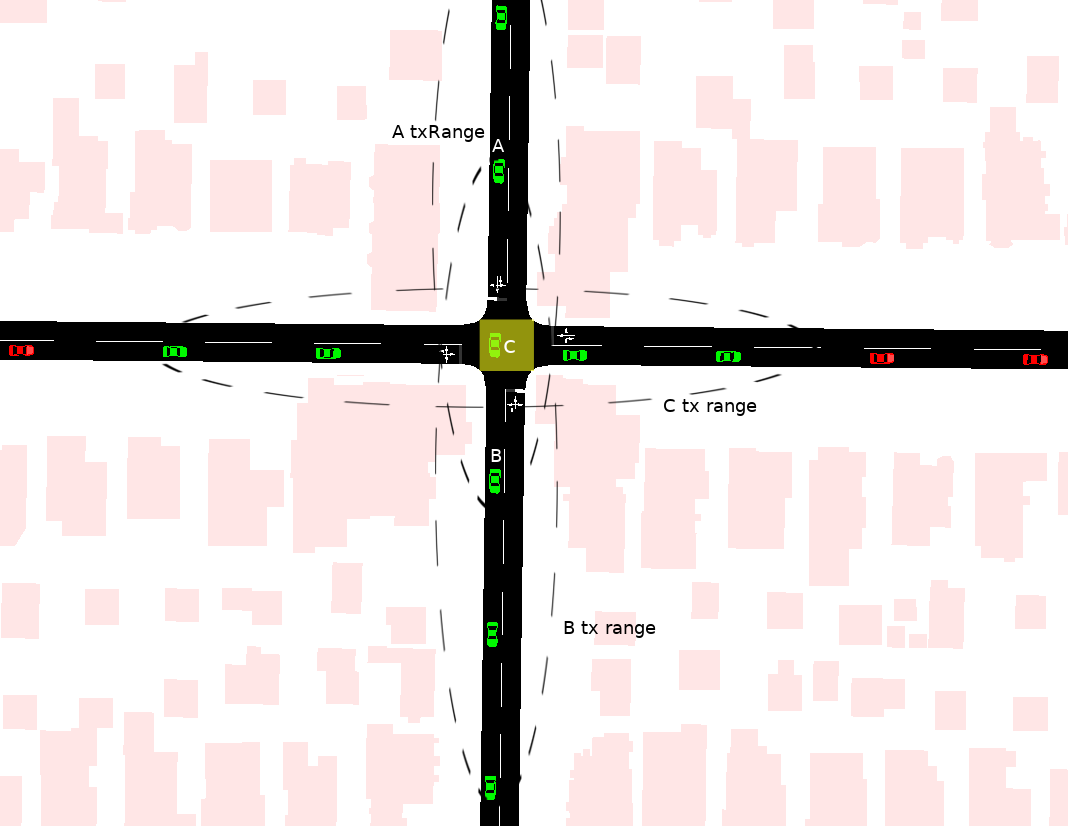
\includegraphics[width=\textwidth]{immagini/fb-junction-1}
			\caption{SJ-Fast-Broadcast Alert Message propagation}
			\label{fig:fb-junction-1}
		\end{figure}
		
		
		The proposed extension works by having nodes inside a junction participate in a second contention with all other vehicles inside the same junction. When the original timer calculated by Fast-Broadcast expires for one of the vehicles inside the junction, it forwards the message. All other vehicles inside the same junction suppress their transmission. This way the propagation can proceed in all directions, while the propagation in the normal direction can proceed without additional delays. Algorithm \ref{alg:sj-alert-message-generation} and \ref{alg:sj-alert-message-forwarding} show the code for SJ-Fast-Broadcast's Broadcast Phase. Estimation Phase's algorithms remain the same as Algorithm \ref{alg:hello-message-sending-2d} and \ref{alg:hello-message-receiving-2d}. Line 4 of Algorithm \ref{alg:sj-alert-message-forwarding} shows that a vehicle suppresses its transmission in one of the following two cases:
		\begin{itemize}
			\item if the vehicle has heard the same broadcast coming from the back and is not inside a junction;
			\item if the vehicle has heard the same broadcast coming from the back, is inside a junction with ID \textit{j} and the sender is also inside the same junction.
		\end{itemize}
		
		\begin{algorithm}[H]
			\begin{algorithmic}[1]
				\State alertMsg.maxRange $\gets$ max(LMR, CMR)
				\State alertMsg.senderPosition $\gets$ retrievePosition()
				\State alertMsg.originPosition $\gets$ retrievePosition()
				\State alertMsg.senderInJunction $\gets$ isSenderInJunction()
				\State alertMsg.junctionId $\gets$ getJunctionId()
				\State transmit(alertMsg)
			\end{algorithmic}
			\caption{SJ-Fast-Broadcast Alert Message generation procedure}
			\label{alg:sj-alert-message-generation}
		\end{algorithm}
		
		\begin{algorithm}[H]
			\begin{algorithmic}[1]
				\State cwnd $\gets$ computeCwnd()
				\State waitTime $\gets$ random(cwnd)
				\State wait(waitTime)
				\If{(sameBroadcastHeardFromBack() $\land$ vehicleNotInJunction()) $\lor$ (sameBroadcastHeardFromBack() $\land$ vehicleInJunction(j) tel$\land$ alertMsg.senderInJunction $\land$ alertMsg.junctionId == j)}
				\State exit()
				\ElsIf{sameBroadcastHeardFromFront()}
				\State restartBroadcastProcedure()
				\Else 
				\State alertMsg.maxRange $\gets$ max(LMBR, CMBR)
				\State alertMsg.senderPosition $\gets$ retrievePosition()
				\State transmit(alertMsg)
				\EndIf 
			\end{algorithmic}
			\caption{SJ-Fast-Broadcast Alert Message forwarding procedure}
			\label{alg:sj-alert-message-forwarding}
		\end{algorithm}
	
		\subsection{Alert Message Header Structure}
			The Hello Message header structure is the same as Figure \ref{fig:fbHelloHeader}, hence it is not reported here. The Alert Message header structure is represented in Figure \ref{fig:sj-fbAlertHeader}.
			
			\begin{figure}[H]
				\centering
				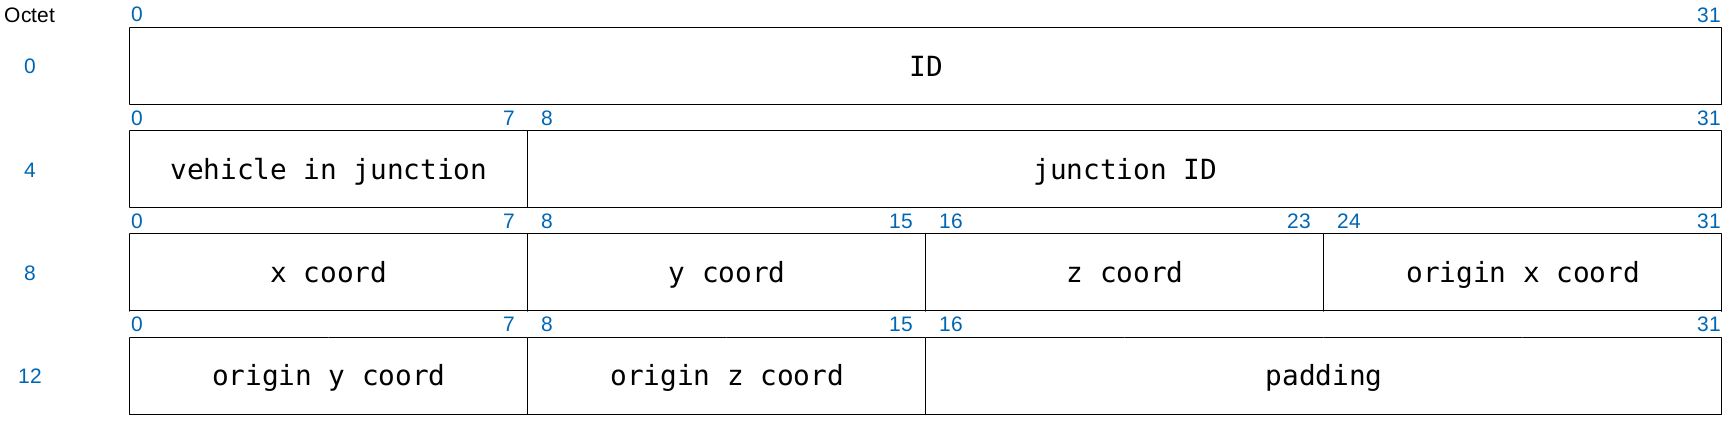
\includegraphics[width=\textwidth]{immagini/sj-fbAlertHeader}
				\caption{SJ-Fast-Broadcast Alert Message header structure}
				\label{fig:sj-fbAlertHeader}
			\end{figure}
			
			The additional fields are the following:
			\begin{itemize}
				\item  \textit{vehicle in junction}: whether the vehicle which is send this Alert Message is inside a junction;
				\item \textit{junction ID}: the ID of the junction the sender is inside.
			\end{itemize}         
% !TEX encoding = UTF-8
% !TEX TS-program = pdflatex
% !TEX root = ../tesi.tex

\chapter{ROFF}
	\label{chapter:roff}

	RObust and Fast Forwarding scheme (ROFF) is a protocol proposed by Hongseok Yoo and Dongkyun Kim in \cite{6906275}. This chapter will present the two main problems tackled by ROFF already introduced in Section \ref{sec:emd}, namely the perfect suppression of redundant transmissions, which will be explained in \ref{ssec:collision-analysis} , and the disuniformity and the costant change in spatial vehicle distribution in VANETs, addressed in section \ref{ssec:latency-analysis}.

	\section{Forwarder Selection Problem}
		\subsection{Collision Analysis}
			\label{ssec:collision-analysis}
			The first problem tackled by ROFF concerns collisions caused by nodes who start to transmit at the same time. This results in a collision in the area resulting from the intersection of the nodes' transmission ranges.
			
			
			Suppose that $S_f=\{f_i | 0 < i \leq N, i \in \mathbb{N} \}$ is the set of PFCs ordered in ascending order by the distance between the previous forwarder and the PFC, where N is the number of PFCs and $f_n$ is the FFC. We define $f_0$ as the previous forwarder.
			Based on the most common idea in existing protocols, ideally a PFC $f_i$ suppresses its scheduled transmission whenever it receives the transmission from $f_N$. In order to achieve suppression, vehicles from $f_i$ to $f_i-1$ should wait until they receive the transmission from $f_N$ before forwarding. If a vehicle forwards the message before having received the transmission from $f_N$, then a collision will occur. As stated in Section \ref{sec:emd}, existing protocols employ a strategy for waiting time assignment by which each PFC calculates its waiting time based on the distance between itself and the previous forwarder (that is $distance = d_{f_i, f_0}$). As a consequence, successful suppression of all PFCs ($f_1$ to $f_{N-1}$, $f_{N-1}$ included) can be achieved only if the timer of $f_{N-1}$ is long enough to detect the transmission from $f_N$. The authors define $minDiff$ as the minimum time difference between $f_N$ and $f_{N-1}$ to prevent $f_{N-1}$ from forwarding.
			
			\begin{figure}[H]
				\centering
				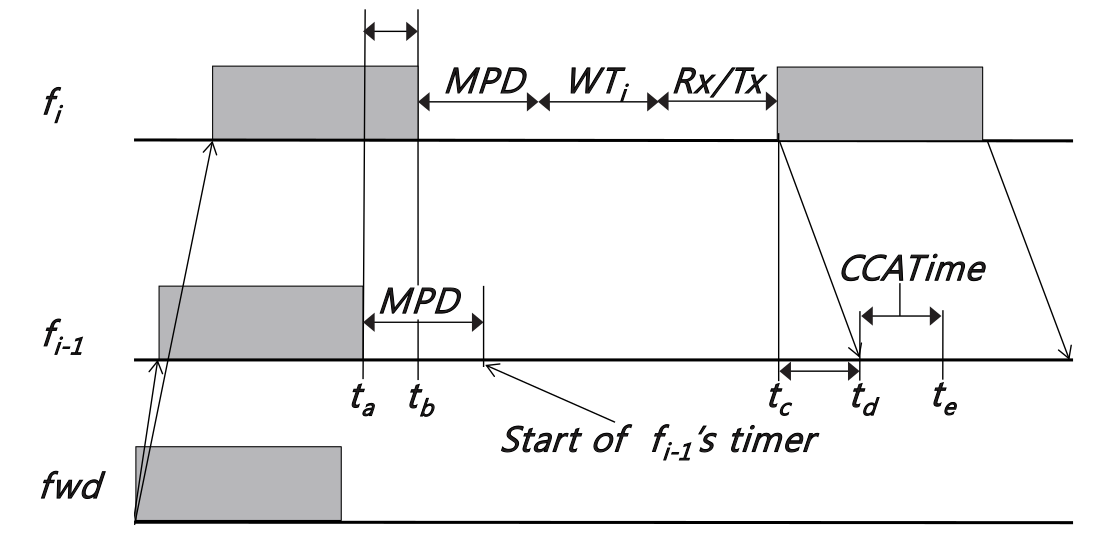
\includegraphics[width=\textwidth]{immagini/minDiff}
				\caption{Definition of $minDiff$ between $f_N$ and $f_{N-1}$ (\cite{6906275})}
				\label{fig:minDiff}
			\end{figure}
		
			\imgrefcap{fig:minDiff} depicts a scenario where $fwd$ is the forwarder and $f_i$ (farther from fwd than $f_{i-1}$) relays the message before $f_{i-1}$. The two vehicles $f_i$ and $f_{i-1}$ complete receiving the message at different times ($t_a$ and $t_b$) due to propagation delay (calculated as $pd = d / s$, where $d$ is the distance between two points in space and $s$ is the wave propagation speed of the medium, i.e., $s=c$, the speed of light, in wireless communication). After reception we have additional amount of time in order to process and retransmit the message:
			\begin{itemize}
				\item each PFC spends MAC Processing Delay (MPD) to process the message and then waits for $WT_i$ calculated according to whichever multi-hop algoritm is being used. As explained previously, this waiting time is inversely proportional to the distance between the PFC and $fwd$;
				\item after timer expiration, each PFC waits for Rx/Tx turnaround time ($Rx/Tx$), in order to switch their interface from reception to transmission mode.
			\end{itemize}
			After $f_i$ has forwarded the message, $f_{i-1}$ starts receiving it at $t_d$, $t_d-t_c$  being equal to $pd{f_{i-1}, f_i}$. The time between the PHY module of $f_{i-1}$ starts reception and the MAC module of the same vehicle is aware of reception is called $CCATime$. Hence, if $f_{i-1}$'s timer expires between $t_a$ and $t_e$, $f_{i-1}$'s transmission will collide with $f_i$'s. In order to accomplish successful suppression, $f_{i-1}$'s timer should not expire  before $t_e$. 
			
			
			Given the fact that propagation delay is not controllable and MPD, $Rx/Tx$ and $CCATime$ are usually standard-defined parameters, an algorithm can only manage the difference between waiting times of $f_i$ and $f_{i-1}$ (represented by $WT_i$ and $WT_{i-1}$ respectively in the following formula).
			To achieve successful suppression, $f_{i-1}$ should wait until the forwarding from $f_i$ is detected by $f_{i-1}$'s MAC layer, so $MPD+WT_{i-1}$ should be greater than $t_e - t_a$. Hence, the formula for $minDiff$ is the following:
			
			\begin{gather}
				\label{eq:minDiff}
				minDiff = (pd_{fwd, f_i} - pd_{fwd, f_{i-1}}) + pd_{f_i, f_{i-1}} + Rx/Tx + CCATime 
			\end{gather}
		
		\subsection{Latency Analysis}
			\label{ssec:latency-analysis}
			The second problem ROFF tries to overcome is the effect of empty space in vehicle distribution on forwarding latency.
			
			The region where PFCs are placed can be defined as \textit{naive forwarding area} (NFA) and is defined as the intersection between:
			\begin{itemize}
				\item the transmission range of a forwarder $fwd$;
				\item the area in the opposite movement direction of the same forwarder $fwd$.
			\end{itemize}
			The distribution of vehicle inside NFA can vary in time; moreover, vehicles are not usually placed at the same distance, so empty spaces of various sizes exist inside the area.
			
			\begin{figure}[H]
				\centering
				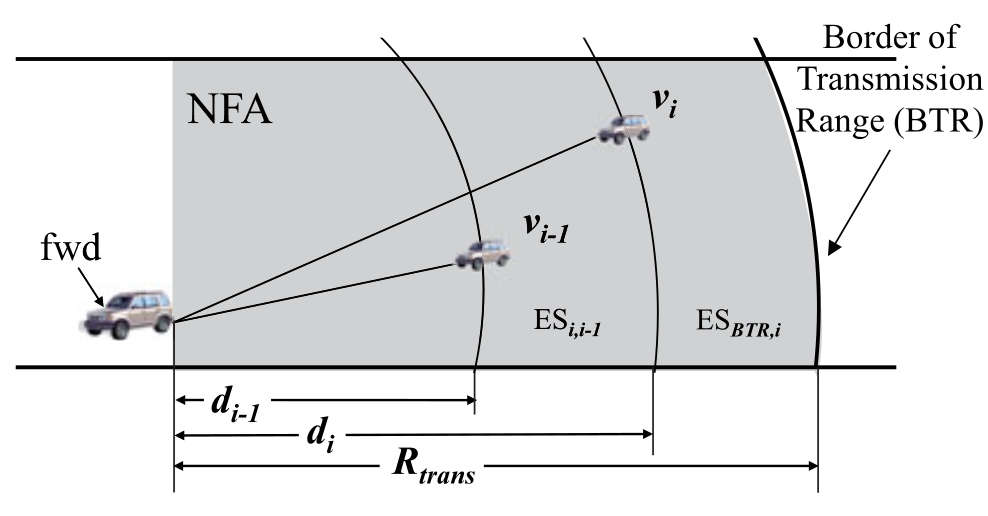
\includegraphics[width=\textwidth]{immagini/emptySpace}
				\caption{Definition of empty space (\cite{6906275})}
				\label{fig:emptySpace}
			\end{figure}
			
			Suppose that $S_v = \{v_i | 0 < i \leq M\}$ is a set of M vehicles inside NFA with vehicles ordered by distance between the vehicle and the previous forwarder in ascending order. Referring to Figure \ref{fig:emptySpace} , the empty space $ES_i,i-1$ between $v_i$ and $v_{i-1}$ is the segment within the two circles centered in $fwd$ with radius $d_{i-1}$ and $d_i$ respectively. Hence, the size of $ES_{i,i-1}$ is equal to $d_i - d_{i-1}$.
			
			
			Large empty spaces have a negative effect on forwarding latency. There is no guarantee that the farthest vehicle from the previous forwarder become the FFC: lossy channel environments, shadowing and other phenomena can make any vehicle within NFA become the forwarder. Suppose that $fwd$ is the previous forwarder and there are two vehicles, $A$ and $B$, inside NFA where A is farther from $fwd$ than $B$, $A$ has not received the transmission from $fwd$ while B has. The empty space $ES_{A,B}$ between $A$ and $B$ influences the forwarding latency:
			\begin{itemize}
				\item if  $ES_{A,B}$ is small, $B$ relays the message after a short waiting time;
				\item if $ES_{A,B}$ is large, $B$ waits needlessly (since there is no other vehicle farther from $fwd$ which has received the message) a large amount of time.
			\end{itemize}
			ROFF aims at resolving the effect of empty spaces by allowing vehicles to choose waiting time directly proportional to their \textit{unique forwarding priority} proportional to the distance between the vehicle and the previous forwarder, instead of using directly such distance in the waiting time computation.
		
	\section{ROFF Algorithm}
		The ROFF algorithm works under the following two assumptions:
		\begin{enumerate}
			\item each vehicle has access to a GPS system and a digital map;
			\item vehicles periodically (e.g., every 100 milliseconds) broadcast a Hello Message containing various information, such as its position, velocity, etc. The period between each Hello Message broadcast is called \textit{Beacon Interval}.
		\end{enumerate}
		The algorithm is composed of three components, as depicted in Figure \ref{fig:roffAlgo}.
	
		\begin{figure}[H]
			\centering
			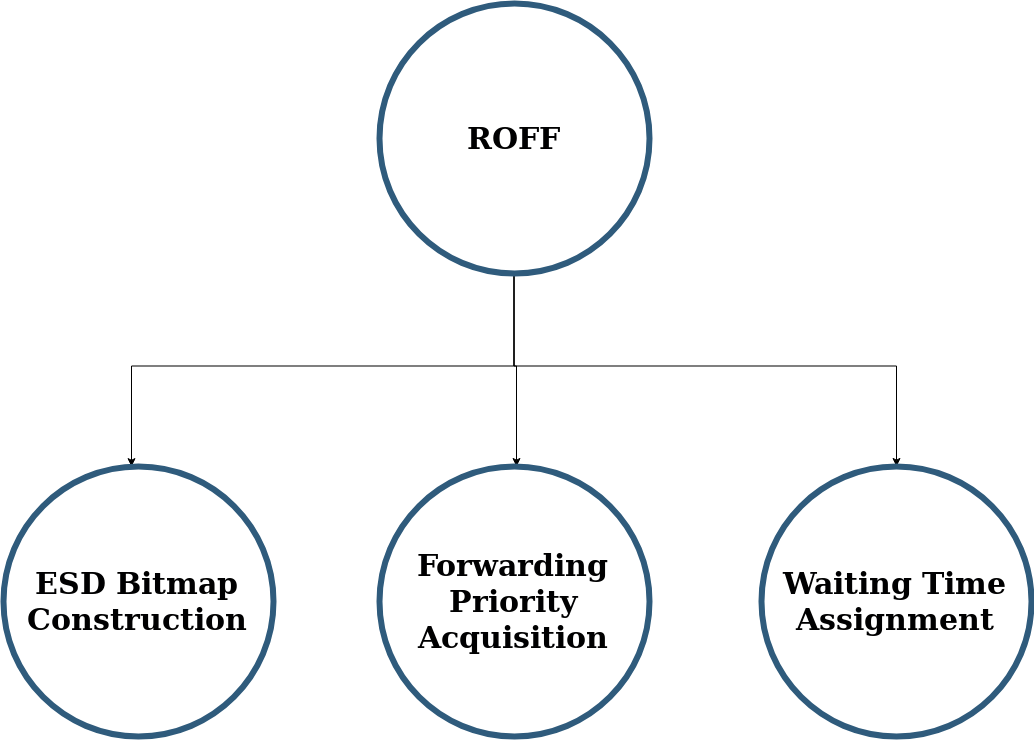
\includegraphics[width=0.6\textwidth]{immagini/roffAlgo}
			\caption{Components of ROFF algorithm}
			\label{fig:roffAlgo}
		\end{figure}
	
		The algorithm in short works as follows (additional information will be given in the following sections):
		\begin{itemize}
			\item when a forwarder relays an Alert Message, it also broadcasts a special structure called ESD Bitmap which describes the empty space distribution within the forwarder's NFA;
			\item PFCs which receive the Alert Message and the ESD Bitmap decide whether they are eligible for contention based on the ESD Bitmap;
			\item eligible PFCs contend by choosing different waiting times based on a unique forwarding priority.
		\end{itemize}
	
		\subsection{ESD Bitmap Construction}
			Upon Hello Message reception, each vehicle uses the data within the message in order to update and maintain a structure called Neighbor Table (NBT) which monitors its local view (i.e., all the vehicles in the neighborhood of said vehicle). Each entry of the NBT contains:
			\begin{itemize}
				\item the ID of the neighbor;
				\item the position of the neighbor;
				\item the reception time of the Hello Message to verify the freshness of information and remove outdates entries.
			\end{itemize}
			An example of Neighbor Table of node with ID 0 is represented in Figure \ref{fig:nbt}.
				
			\begin{figure}[H]
				\centering
				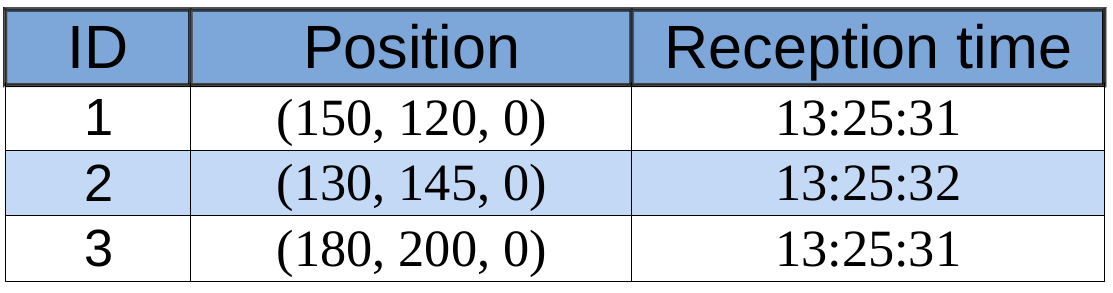
\includegraphics[width=0.7\textwidth]{immagini/nbt}
				\caption{Example of Neighbor Table of node with ID 0}
				\label{fig:nbt}
			\end{figure}
			Thanks to the NBT, the forwarder can advertise its neighborhood to other vehicles. We can define the set of neighbors detected by the forwarder as its \textit{local view}. If a vehicle who receives an Alert Message is not present inside the local view of the forwarder, then that vehicle cannot participate in contention.
			
			
			The NBT could be piggybacked as-is on the Alert Message, but the authors of ROFF identified some problems with this solution, such as the great overhead caused by the size of IDs. Hence, the proposed solution consists in compressing the NBT in a bitmap-like structure called ESD Bitmap. 
			
			
			In order to build the ESD Bitmap, first of all the forwarder measures the distance between itself and each of its neighbors listed in the NBT. Due to GPS granularity, distances are expressed at meter-level and can be represented with non-negative integers.
			
			\begin{figure}[H]
				\centering
				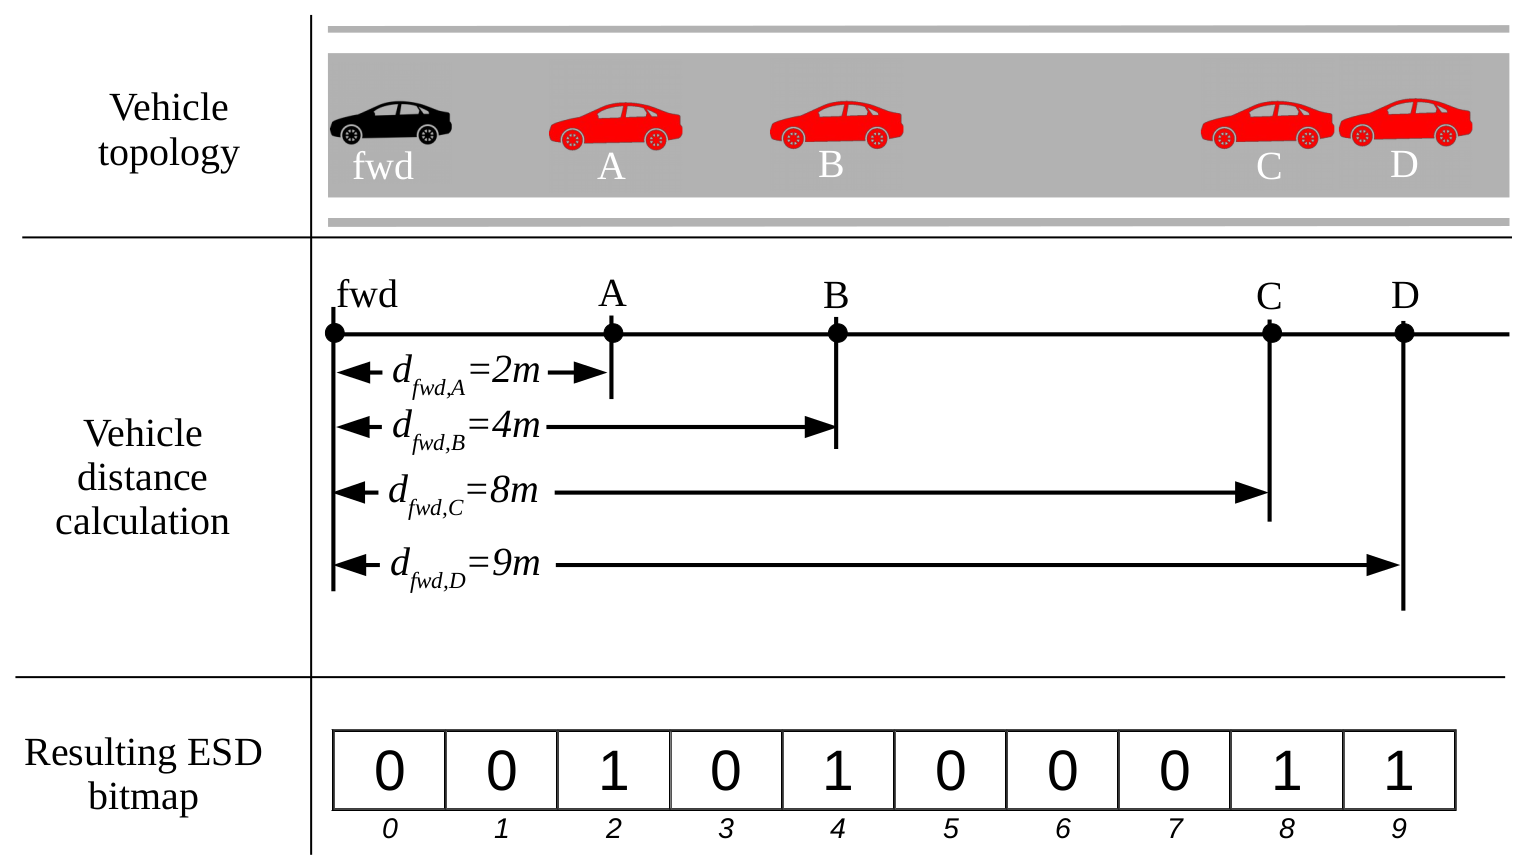
\includegraphics[width=\textwidth]{immagini/esdBitmapConstruction}
				\caption{ESD Bitmap construction with \textit{k} = 1}
				\label{fig:esdBitmapConstruction}
			\end{figure}
			
			After distance measurement, \textit{fwd} builds a bitmap to represent the measured distances by setting the \textit{i-th} bit to either:
			\begin{itemize}
				\item 1 if there is a PFC distant $d$ from \textit{fwd} such that $k * i \leq d \leq k * ( i + 1 ) - 1$;
				\item 0 otherwise.
			\end{itemize} 
			The parameter \textit{k}, called \textit{distance range}, identifies how many distances can be identified by the same bit in the ESD Bitmap. This parameter can be controlled to manage the compression level and the accuracy of the Bitmap. Increasing \textit{k} decreases the number of bits of the Bitmap, but every bit will identify \textit{k} different distances, hence losing precision.
			Figure \ref{fig:esdBitmapConstruction} shows the construction of an ESD Bitmap using $k = 1$.
			
			
			An ESD Bitmap using $k = 2$ is show in Figure \ref{fig:esdBitmapConstructionK2}. It is possible to see that the bit in position 4 represents distances $d$ such that $8 \leq d \leq 9$. 
			
			\begin{figure}[H]
				\centering
				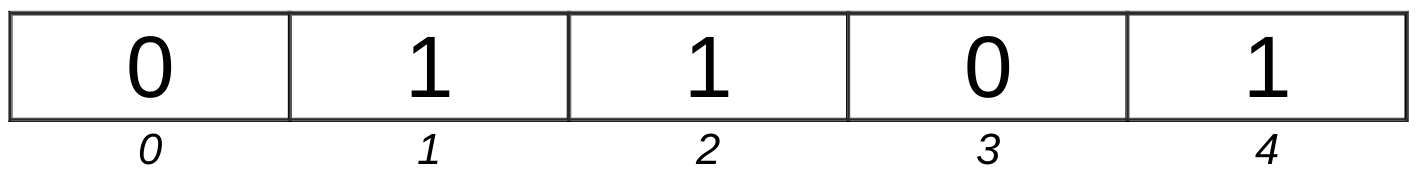
\includegraphics[width=\textwidth]{immagini/esdBitmapConstructionK2}
				\caption{Resulting ESD Bitmap with \textit{k} = 2}
				\label{fig:esdBitmapConstructionK2}
			\end{figure}
		
		\subsection{Forwarding Priority Acquisition}
			Whenever a PFC $f_i$ receives the Alert Message with included the ESD Bitmap from $fwd$, it checks whether the distance between itself and the previous forwarder is listed inside the bitmap (i.e., $f_i$ checks whether the bit in position $d(fwd, f_i)$ in the bitmap is equal to 1, assuming $k = 1$). If so, $f_i$ can participate in contention since it is inside the \textit{local view} of $fwd$. Otherwise, is cannot participate in contention to forward the Alert Message.
			
			
			After $f_i$ has entered contention, it can calculate its own forwarding priority based on the distances express by the ESD Bitmap. These distances are the distances of every other PFC which can participate in contention. Assuming that $L_{dist}$ is the list of distances ordered in ascending order and $distance = d(fwd, f_i)$, $f_i$'s forwarding priority is set as the rank of $distance$ inside $L_{dist}$. This way PFCs that are farther away from $fwd$ are assigned a higher forwarding priority, while PFCs nearer $fwd$ are assigned a lower forwarding priority.
			
			
			ROFF avoids assigning the same priority to two different PFCs by a technique called \textit{ID-based contention}. Using this technique, whenever a PFC $f_i$ receives an Alert Message it checks whether its NBT contains another vehicle $f_j$ whose distance from $fwd$ is the same as $f_i$'s (hence the distance is identified by the same bit in the bitmap). If so, $f_i$ participates in contention only if its ID is higher than the ID of $f_j$. In other words, if inside $f_i$'s NBT there exists an entry for $f_j$ such that $d(fwd, f_i) = d(fwd, f_j)$ and $ID_{f_j} > ID_{f_i}$, then $f_i$ defers its transmission. Figure \ref{fig:idBasedContention} depicts a scenario where node A does not participate in contention due to ID-based contention.
	
			\begin{figure}[H]
				\centering
				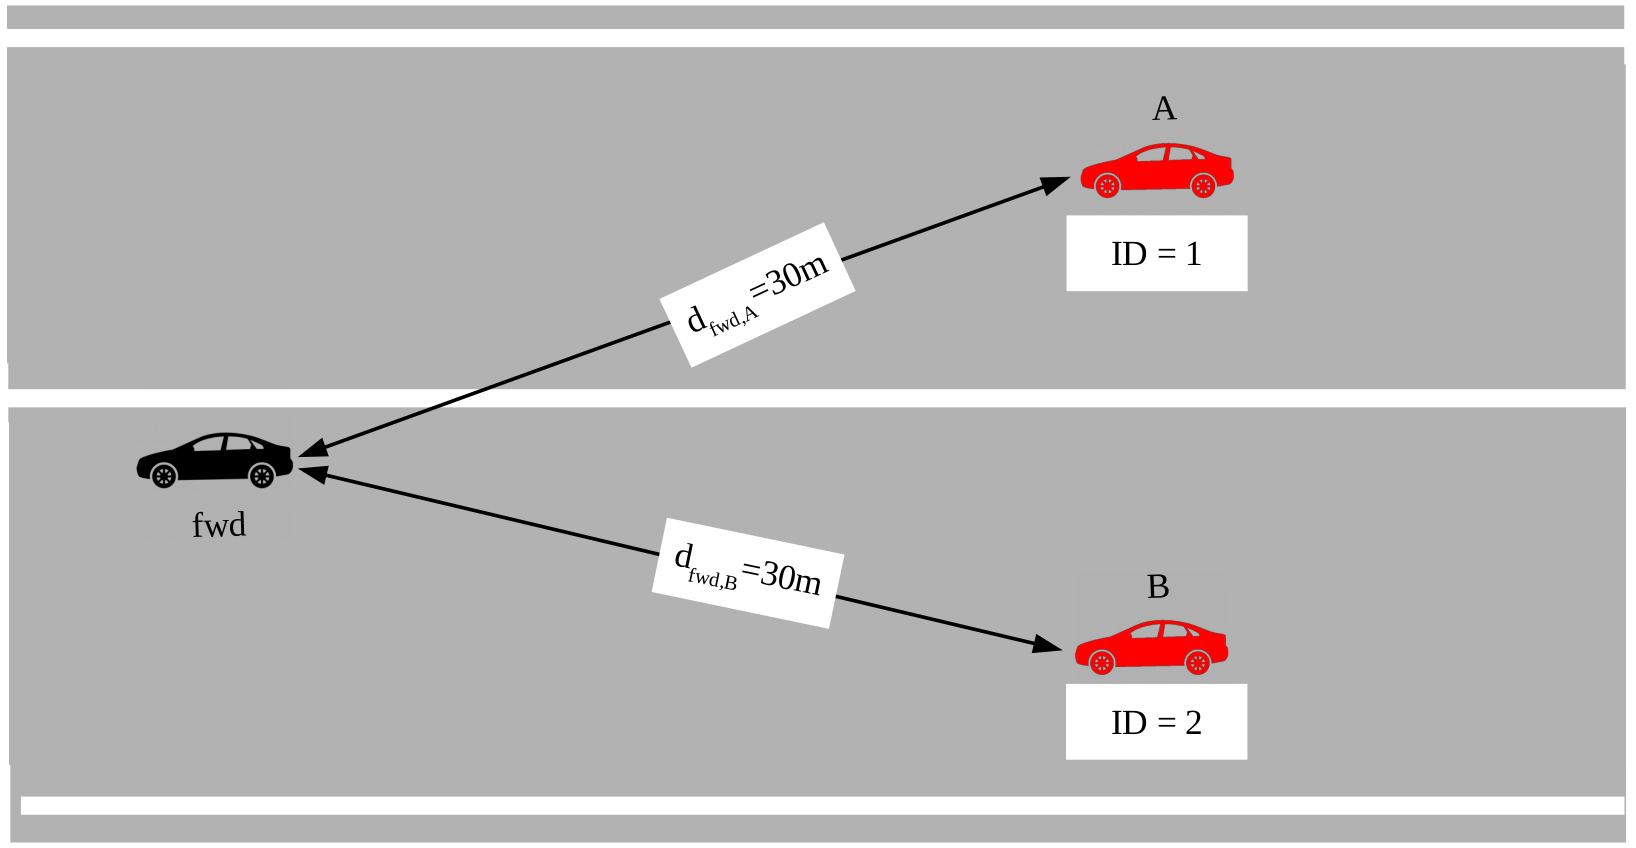
\includegraphics[width=\textwidth]{immagini/idBasedContention}
				\caption{ID-based contention: node A defers its transmission}
				\label{fig:idBasedContention}
			\end{figure}
		
		\subsection{Waiting Time Assignment}
			Once forwarding priorities are determined, ROFF assigns a waiting time to each vehicle that is inversely proportional to the priority. Letting $PFC(i)$ be the PFC with forwarding priority $i$ and $WT_p$ the waiting time of PFC $p$, in order to achieve successful suppression of transmission by $PFC(i-1)$, the waiting time of $PFC(i-1)$ should be at least longer by $minDiff_{PFC(i), PFC(i-1)}$ than waiting time of $PFC(i)$ (i.e., $WT_{PFC(i-1)} \geq WT_{PFC(i)} + minDiff_{PFC(i), PFC(i-1)})$. Hence, the waiting time of $PFC(k)$ is the sum of $minDiff$s (calculated using Equation \ref{eq:minDiff}) between PFCs with forwarding priorities lower than $k$, as shown in Equation \ref{eq:waitingTimeAssignment}. The PFC with top priority (being equal to 1) broadcasts immediately and does not have to wait any time.
			
			\begin{gather}
				WT_{PFC(k)} = \sum_{i=2}^{k} minDiff_{PFC(i),PFC(i-1)} (k \geq 2)
				\label{eq:waitingTimeAssignment}
			\end{gather}
			
			Figure \ref{fig:waitingTimeAssignment} shows the application of \ref{eq:waitingTimeAssignment} in the scenario represented in Figure \ref{fig:esdBitmapConstruction}.
			
			\begin{figure}[H]
				\centering
				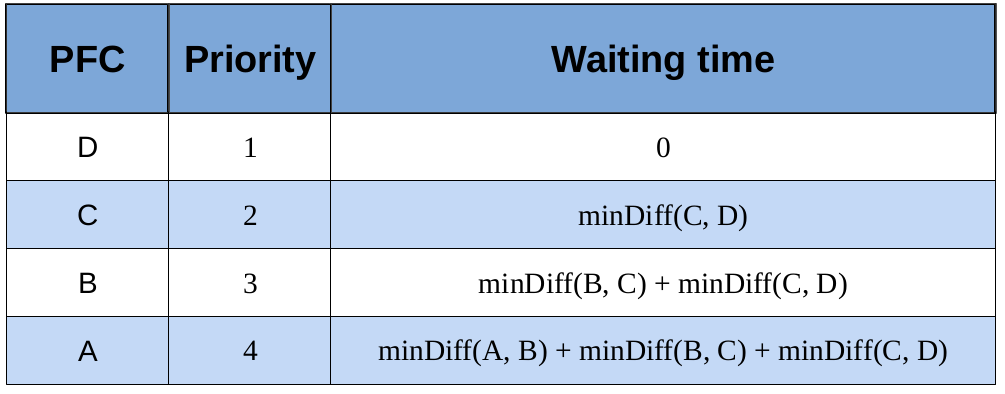
\includegraphics[width=\textwidth]{immagini/waitingTimeAssignment}
				\caption{Waiting time assignment based on vehicle distribution depicted in Figure \ref{fig:esdBitmapConstruction}}
				\label{fig:waitingTimeAssignment}
			\end{figure}
			
			When calculating $minDiff$ as explained in Section \ref{ssec:collision-analysis}, $MPD$, $Rx/Tx$ and $CCATime$ are fixed system parameters; the only variables are propagation delays between vehicles, which are dependent on distance. Since coordinates are not included in the ESD Bitmap (only distances are), each PFC needs to identify the coordinates of the previous forwarder's neighbors. In other words, whenever a PFC $f_i$ receives the ESD Bitmap from $fwd$ and calculates its own waiting time, it checks for each distance $dist$ in $L_{dist}$ whether there is a vehicle $f_j$ distant $dist$ from $fwd$ (i.e., $d(fwd, f_j) = dist$) inside its own NBT. If such vehicle exists, then $f_i$ uses $f_j$'s coordinates in the propagation delay (hence $minDiff$) calculation, otherwise it disregards $dist$ in the computation since possibly there is no vehicle distant $dist$ from $fwd$ in $f_i$'s local view.
			
	\section{Multiple dimensions extension}
		
		In the original work \cite{6906275}, ROFF has been implemented in the network simulator ns-2. Since retrieval of the original code has proven to be impossible, part of this thesis concerned the implementation of ROFF in ns-3. Moreover, the original article focuses only on 1D message propagation along a strip-shaped area. This work proposes a 2D and 3D extension of ROFF based on the idea of Fast-Broadcast presented in Section \ref{sec:fb-multiple-dimensions}. The main addition to the original algorithms consists in the suppression of scheduled transmissions only when an Alert Message is heard coming from a vehicle farther from the initial sender than the current vehicle. More in detail, if $fwd$ is the origin of the Alert Message, $A$ is the previous forwarder and $B$ is a PFC with a scheduled transmission. $B$ will suppress its transmission only if it hears an Alert Message coming from $D$ such that $d_{fwd, D} > d_{fwd, B}$.
		Algorithm \ref{alg:roff-hello-message-sending}, \ref{alg:roff-hello-message-receiving}, \ref{alg:roff-alert-message-generation} and \ref{alg:roff-alert-message-forwarding} show ROFF's phases in detail.
		
		\begin{algorithm}[H]
			\begin{algorithmic}[1]
				\ForEach{beaconInterval}
				\State helloMsg.ID $\gets$ retrieveID()
				\State helloMsg.senderPosition $\gets$ retrievePosition()
				\State transmit(helloMsg)
				\EndFor
			\end{algorithmic}
			\caption{Hello message sending procedure for 2D}
			\label{alg:roff-hello-message-sending}
		\end{algorithm}
	
		\begin{algorithm}[H]
			\begin{algorithmic}[1]
				\State id $\gets$ helloMsg.ID
				\State sp $\gets$ helloMsg.senderPosition
				\State time $\gets$ currentTime()
				\State addNBTEntry(id, sp, time)
			\end{algorithmic}
			\caption{Hello message receiving procedure for 2D}
			\label{alg:roff-hello-message-receiving}
		\end{algorithm}
		
		\begin{algorithm}[H]
			\begin{algorithmic}[1]
				\State esdBitmap $\gets$ createEsdBitmap(NBT)
				\State alertMsg.esdBitmapSize $\gets$ esdBitmap.size
				\State alertMsg.esdBitmap $\gets$ esdBitmap
				\State alertMsg.senderPosition $\gets$ retrievePosition()
				\State alertMsg.originPosition $\gets$ retrievePosition()
				\State transmit(alertMsg)
			\end{algorithmic}
			\caption{Alert Message generation procedure for 2D}
			\label{alg:roff-alert-message-generation}
		\end{algorithm}
		
		\begin{algorithm}[H]
			\begin{algorithmic}[1]
				\State esdBitmap $\gets$ alertMsg.esdBitmap
				\If{vehicleNotPresentInEsd() $\lor$ lostIDContention()}
				\State exit()
				\Else
				\State listOfDistances $\gets$ computeListOfDistances(esdBitmap)
				\State myPosition $\gets$ retrievePosition()
				\State senderPosition $\gets$ alertMsg.senderPosition
				\State dist $\gets$ distance(myPosition, senderPosition)
				\State myRank $\gets$ getRank(dist, listOfDistances)
				\State wait $\gets$ computeWaitTime(myRank)
				\If{sameBroadcastHeardFromBack()}
				\State exit()
				\ElsIf{sameBroadcastHeardFromFront()}
				\State restartBroadcastProcedure()
				\Else
				\State esdBitmap $\gets$ createEsdBitmap(NBT)
				\State alertMsg.esdBitmapSize $\gets$ esdBitmap.size
				\State alertMsg.esdBitmap $\gets$ esdBitmap
				\State alertMsg.senderPosition $\gets$ retrievePosition()
				\State transmit(alertMsg)
				\EndIf 
				\EndIf
			\end{algorithmic}
			\caption{Alert Message forwarding procedure for 2D}
			\label{alg:roff-alert-message-forwarding}
		\end{algorithm}
		
		
		\subsection{Hello Message Header Structure}
			The Hello Message header structure is represented in Figure \ref{fig:roffHelloHeader}.
				
			\begin{figure}[H]
				\centering
				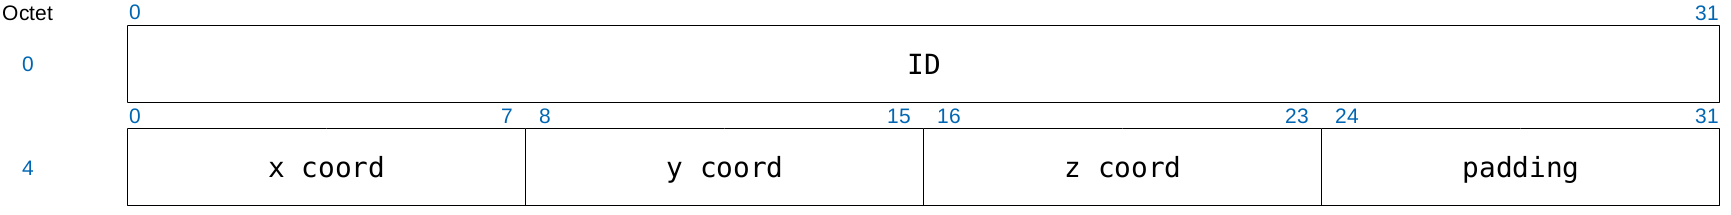
\includegraphics[width=\textwidth]{immagini/roffHelloHeader}
				\caption{ROFF Hello Message header structure}
				\label{fig:roffHelloHeader}
			\end{figure}
				
			The fields contained in the Hello Message are the following:
			\begin{itemize}
				\item \textit{ID}: unique ID of the Hello Message's sender;
				\item \textit{x coord}, \textit{y coord} and \textit{z coord}: coordinates of the Hello Message's sender.
			\end{itemize}
		
		\subsection{Alert Message Header Structure}
			The Alert Message header structure is represented in Figure \ref{fig:roffAlertHeader}.
			
			\begin{figure}[H]
				\centering
				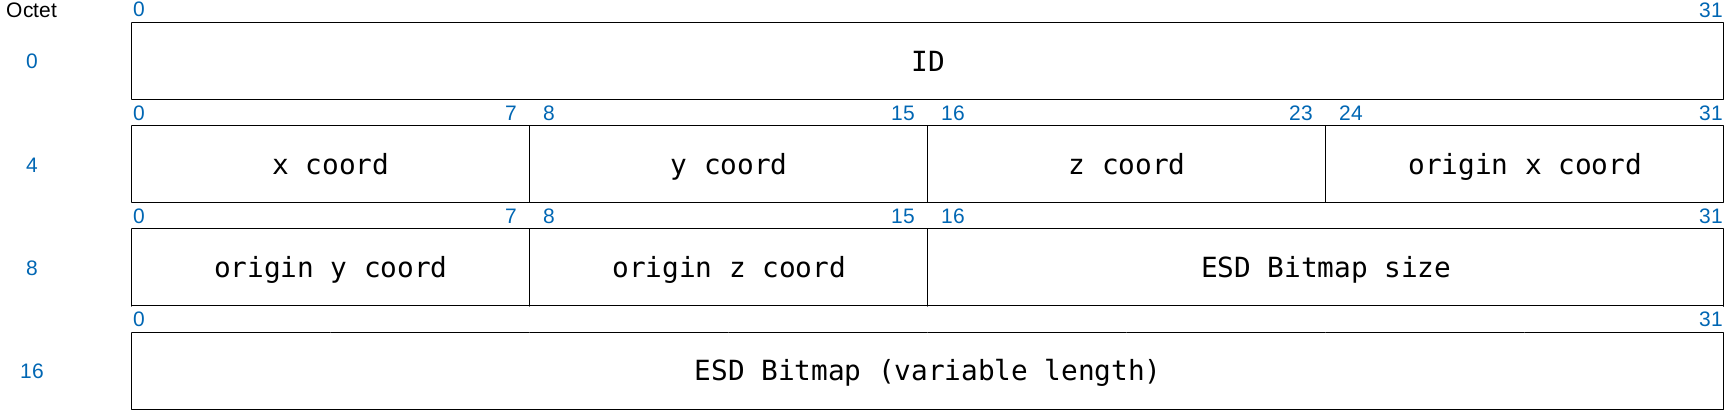
\includegraphics[width=\textwidth]{immagini/roffAlertHeader}
				\caption{ROFF Alert Message header structure}
				\label{fig:roffAlertHeader}
			\end{figure}
			
			The fields contained in the Alert Message are the following:
			\begin{itemize}
				\item \textit{ID}: unique ID of the Alert Message's sender (or forwarder);
				\item \textit{x coord}, \textit{y coord} and \textit{z coord}: coordinates of the Alert Message's forwarder;
				\item \textit{origin x}, \textit{origin y} and \textit{origin z coord}: coordinates where the Alert initially originated from;
				\item \textit{ESD Bitmap size}: field which indicates how many bytes the ESD Bitmap occupies;
				\item \textit{ESD Bitmap}: the ESD Bitmap itself, with variable length.
			\end{itemize}
	
	\section{Smart Junction ROFF (SJ-ROFF)}
		Since ROFF does not consider junctions in the default algorithm, the proposal explained in Section \ref{sj:fb} could also bring benefits to it. Hence, we have implemented a Smart Junction variant of ROFF (called SJ-ROFF) following the logic of SJ-Fast-Broadcast. The modifications to the base algorithm are fairly simple: two fields have been added to the Alert Message Header to indicate whether the sender is located within a junction (and the ID of the junction, if it is). Algorithm \ref{alg:sj-roff-alert-message-generation} and \ref{alg:sj-roff-alert-message-forwarding} show the updated functionalities of Alert Message creation and forwarding. Hello Message algorithms are unchanged.
		
		\begin{algorithm}[H]
			\begin{algorithmic}[1]
				\State esdBitmap $\gets$ createEsdBitmap(NBT)
				\State alertMsg.esdBitmapSize $\gets$ esdBitmap.size
				\State alertMsg.esdBitmap $\gets$ esdBitmap
				\State alertMsg.senderPosition $\gets$ retrievePosition()
				\State alertMsg.originPosition $\gets$ retrievePosition()
				\State alertMsg.senderInJunction $\gets$ isSenderInJunction()
				\State alertMsg.junctionId $\gets$ getJunctionId()
				\State transmit(alertMsg)
			\end{algorithmic}
			\caption{Alert Message generation procedure for 2D}
			\label{alg:sj-roff-alert-message-generation}
		\end{algorithm}
		
		\begin{algorithm}[H]
			\begin{algorithmic}[1]
				\State esdBitmap $\gets$ alertMsg.esdBitmap
				\If{vehicleNotPresentInEsd() $\lor$ lostIDContention()}
				\State exit()
				\Else
				\State listOfDistances $\gets$ computeListOfDistances(esdBitmap)
				\State myPosition $\gets$ retrievePosition()
				\State senderPosition $\gets$ alertMsg.senderPosition
				\State dist $\gets$ distance(myPosition, senderPosition)
				\State myRank $\gets$ getRank(dist, listOfDistances)
				\State wait $\gets$ computeWaitTime(myRank)
				\If{(sameBroadcastHeardFromBack() $\land$ vehicleNotInJunction()) $\lor$ (sameBroadcastHeardFromBack() $\land$ vehicleInJunction(j) $\land$ alertMsg.senderInJunction $\land$ alertMsg.junctionId == j)}
				\State exit()
				\ElsIf{sameBroadcastHeardFromFront()}
				\State restartBroadcastProcedure()
				\Else
				\State esdBitmap $\gets$ createEsdBitmap(NBT)
				\State alertMsg.esdBitmapSize $\gets$ esdBitmap.size
				\State alertMsg.esdBitmap $\gets$ esdBitmap
				\State alertMsg.senderPosition $\gets$ retrievePosition()
				\State transmit(alertMsg)
				\EndIf 
				\EndIf
			\end{algorithmic}
			\caption{Alert Message forwarding procedure for 2D}
			\label{alg:sj-roff-alert-message-forwarding}
		\end{algorithm}
	
		\subsection{Alert Message Header Structure}
			The Hello Message header structure is the same as Figure \ref{fig:roffHelloHeader}, hence it is not reported here. The Alert Message header structure is represented in Figure \ref{fig:sj-roffAlertHeader}.
		
		\begin{figure}[H]
			\centering
			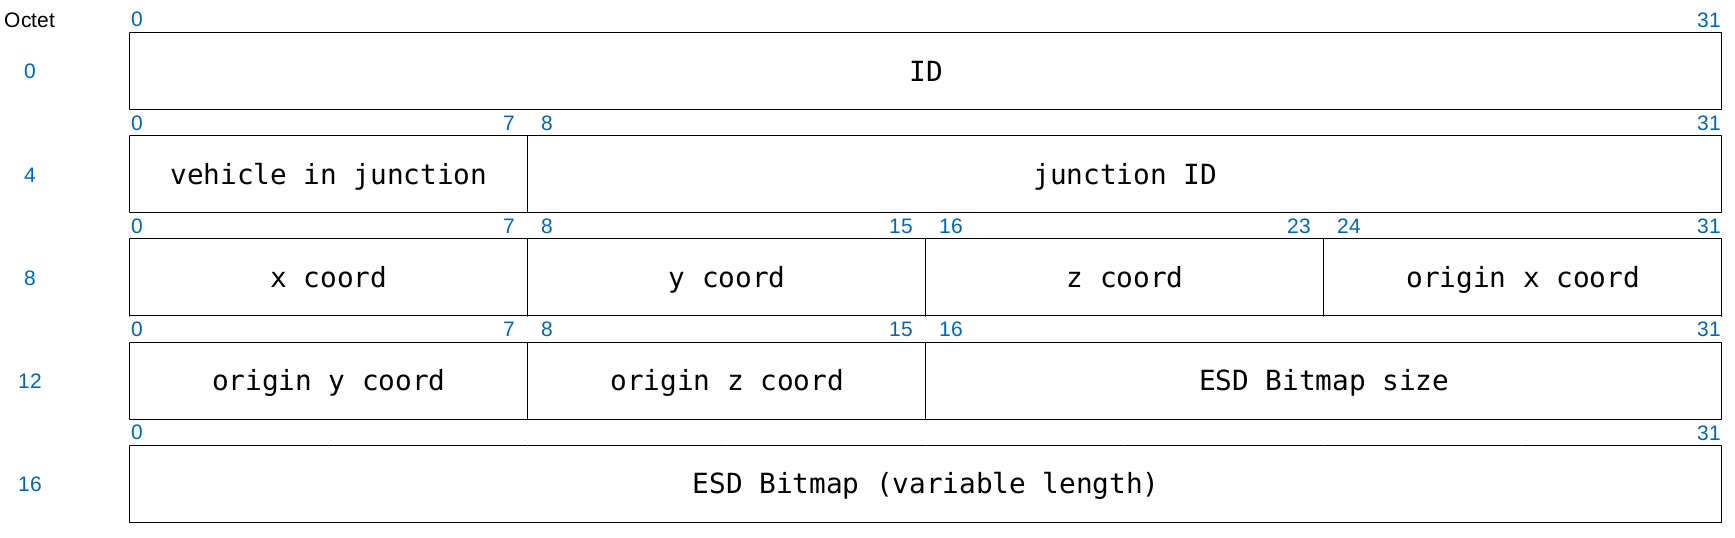
\includegraphics[width=\textwidth]{immagini/sj-roffAlertHeader}
			\caption{SJ-ROFF Alert Message header structure}
			\label{fig:sj-roffAlertHeader}
		\end{figure}
		
		The additional fields are the following:
		\begin{itemize}
			\item  \textit{vehicle in junction}: whether the vehicle which has forwarded this Alert Message is inside a junction;
			\item \textit{junction ID}: the ID of the junction the sender is inside.
		\end{itemize}
		
	
		
		
		
	      
% !TEX encoding = UTF-8
% !TEX TS-program = pdflatex
% !TEX root = ../tesi.tex


\chapter{Tools and applications}
	\section{Network Simulator 3}
		Network Simulator 3 (ns-3) is a discrete-event network simulator for Internet systems, targeted primarily for research and educational use. ns-3 is free software, licensed under the GNU GPLv2 license, and is publicly available for research, development, and use.
		
		
		ns-3 development began in 2006 by a team lead by Tom Henderson, George Riley, Sally Floyd and Sumit Roy. Its first version was released on June 30, 2008. 
		
		
		ns-3 is the successor of ns-2, released in 1989. The fact that the former was built from scratch makes it impossible to have backward compatibility. In fact, ns-2 used oTCL scripting language to describe network topologies and C++ to write the core of the simulation. This choice was due to avoid the very time consuming C++ code recompilation, exploiting the interpreted language oTCL. ns-2 mixed the \jquote{fast to run, slow to change} C++ with the \jquote{slow to run, fast to change} oTCL language. Since compilation time was not an issue with modern computing capabilities, ns-3 developers chose to utilize exclusively C++ code (and optional Python bindings) to develop simulations.
		
		\subsection{Modules and module structure}
		ns-3 is composed of various modules, which are groups of classes, examples and tests each related to a certain feature. The components of a module work in a cohesive way in order to offer APIs to other modules and users. Some examples of built-in modules are:
		\begin{itemize}
			\item WiFi;
			\item AODV; 
			\item CSMA.
		\end{itemize}
		The obstacle shadowing propagation loss model and the Fast Broadcast algorithm have been implemented as modules too.
		
		
		Modules follow a prototypical structure in order to promote clarity and offer built-in documentation. \imgrefcap{fig:ns-3-module} shows the typical module structure.
		
		\begin{figure}[H]
			\centering
			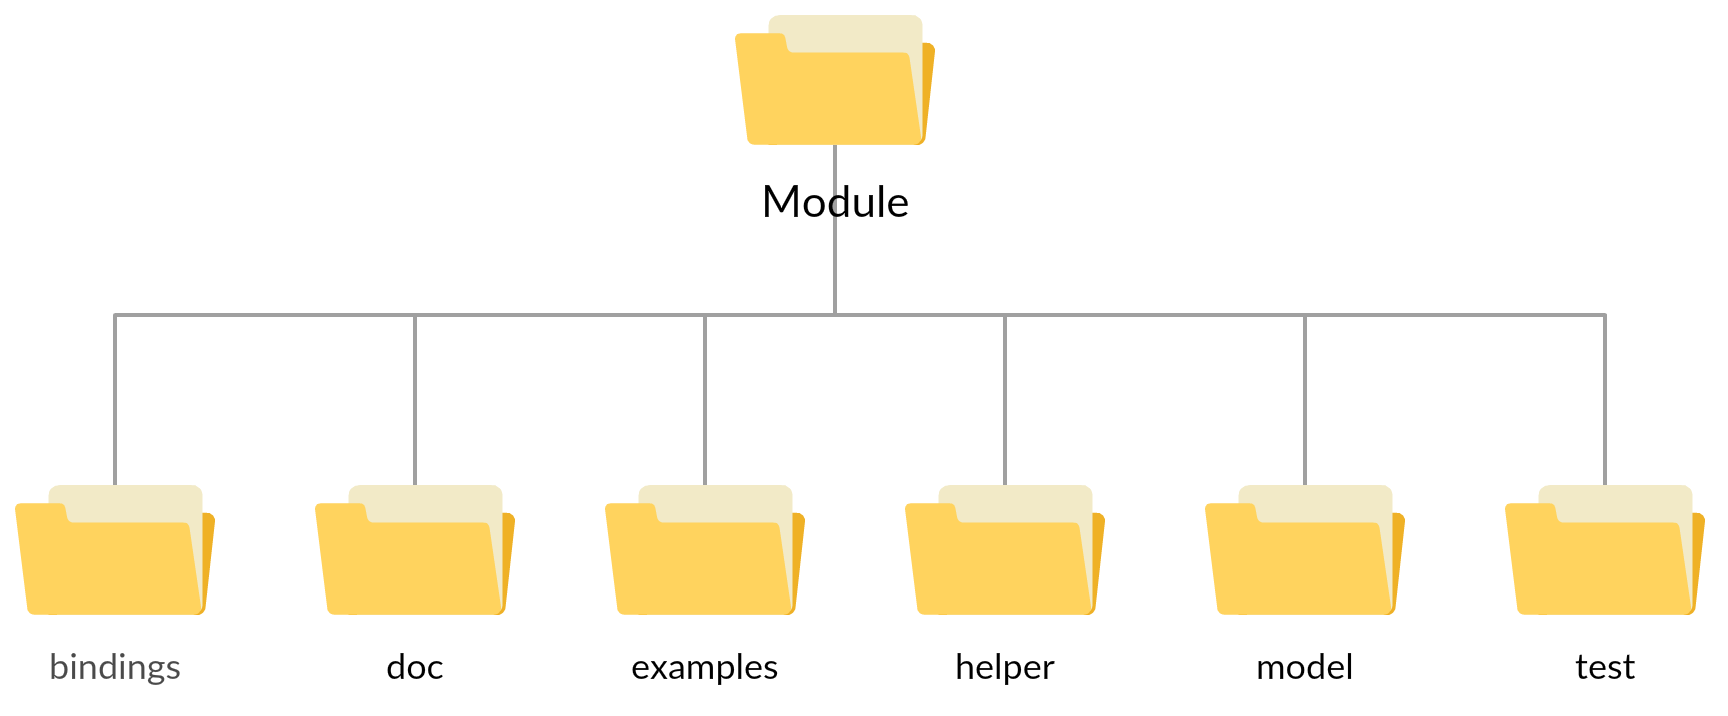
\includegraphics[width=\textwidth]{immagini/ns-3-module}
			\caption{ns-3 module structure}
			\label{fig:ns-3-module}
		\end{figure}
		
		The following directories can be found inside a module's root directory:
		\begin{itemize}
			\item \textbf{bindings:} Python bindings used to make the module's API compatible with Python;
			\item \textbf{doc:} documentation of the module;
			\item \textbf{examples:} examples and proof of concepts of what can be done using the module;
			\item \textbf{helper:} higher level APIs to make the module easier to use;
			\item \textbf{model:} headers and source files which implement the module's logic; 
			\item \textbf{test:} test suite and test cases to test the module.
		\end{itemize}
	
		\subsection{Key elements}
			The element at the base of ns-3 is called \textit{node}, instance of \texttt{ns3::Node}. A node can be thought of as a shell of a computer. Various other elements can be added to nodes, such as:
			\begin{itemize}
				\item NetDevices (e.g. \acrshort{nica}s, which enable nodes to communicate over \textit{channels});
				\item protocols;
				\item applications. 
			\end{itemize}
			The applications implement the logic of a simulation. For example, the \texttt{UdoEchoClientApplication} and \texttt{UdpEchoServerApplication} can be used to implement a client/server application which exchange and print the packets' content over the network. The Fast Broadcast protocol has been implemented as an application as well.
			
		
		The \textit{channels} model various type of transmission media, such as the wired and the wireless ones.
	
		\subsection{Structure of a simulation}
			A simulation can be implemented in many ways, but in most cases the following steps are executed:
			\begin{itemize}
				\item manage command line arguments (e.g. number of nodes to consider in the simulation, transmission range, etc.);
				\item initialize all the necessary fields in classes;
				\item create nodes;
				\item set up physical and MAC layers;
				\item set up link layer, routing protocols and addresses;
				\item configure and install applications on nodes;
				\item position nodes and (optionally) give them a mobility model;
				\item schedule user defined events, such as transmissions of packets;
				\item start the simulation;
				\item collect and manage output data.
			\end{itemize}
		
		\subsection{NetAnim}
			Netanim is an offline animator tool based on the Qt toolkit. It collects an XML tracefile during the execution of a simulation and can be used to animate the simulation, analyzing packet transmissions and contents.
			
			\begin{figure}[H]
				\centering
				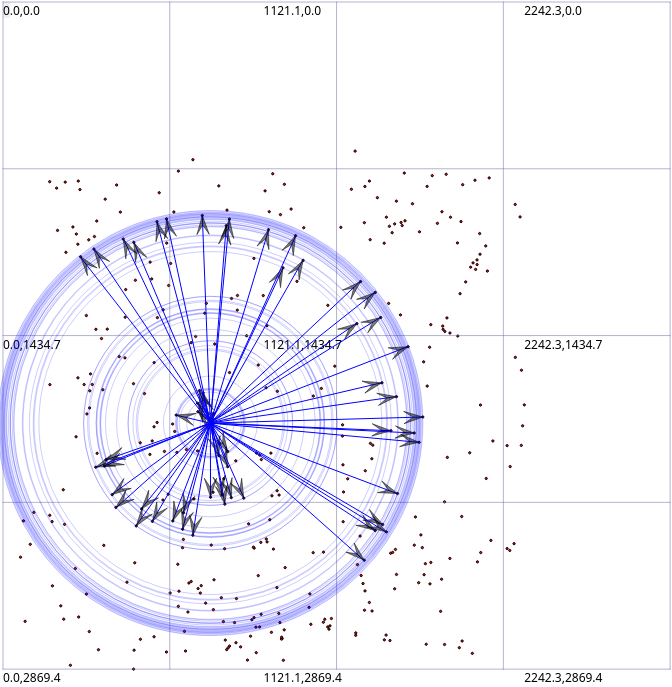
\includegraphics[scale=0.38]{immagini/netanim}
				\caption{Packet transmission in NetAnim}
				\label{fig:netanim}
			\end{figure}
	
	\section{Simulation of Urban MObility}
		\label{sec:sumo}
		Simulation of Urban MObility is an open-source road traffic simulation package. It is written in C++ and licensed under GPLv3. 
		
		
		It offers different tools to analyze and manage real maps from the urban mobility point of view, including pedestrian movement and various types of vehicles.
		
		
		The original work, starting from real maps obtained from OpenStreetMap (OSM), \cite{ROM2017} utilized SUMO to produce two files:
		\begin{enumerate}
			\item a \texttt{.poly} file using the SUMO tool \textit{Polyconvert}. This file contains information about all the obstacles, such as buildings, useful for the Obstacle Shadowing module;
			\item a \texttt{.ns2mobility} file using the SUMO tool \textit{TraceExporter}. This file contains information about the vehicles and their positioning. 
		\end{enumerate}
		The process of generating these two files necessary for ns-3 simulations requires some intermediate steps. The full process is represented in \imgref{fig:sumo-process}. 
		
		The original work considered a only a distance of 25 meters between vehicles; this work considers various distances, ranging from 15 to 45 meters. \imgrefcap{fig:sumo-distances}  shows the same scenario (Padua) with different distances between vehicles.
		
		\begin{figure}[H]
			\centering
			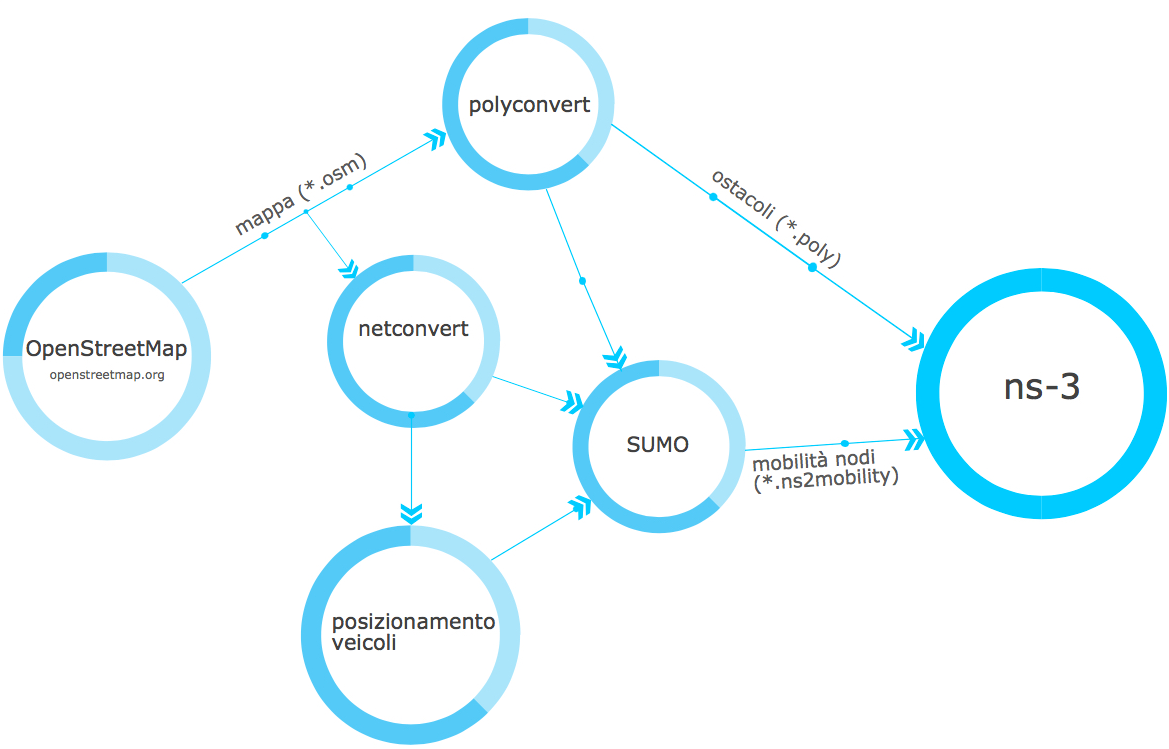
\includegraphics[width=\textwidth]{immagini/sumo-process}
			\caption{Steps to generate necessary files using SUMO (\cite{ROM2017})}
			\label{fig:sumo-process}
		\end{figure}
		
		\begin{figure}[H]
			\centering
			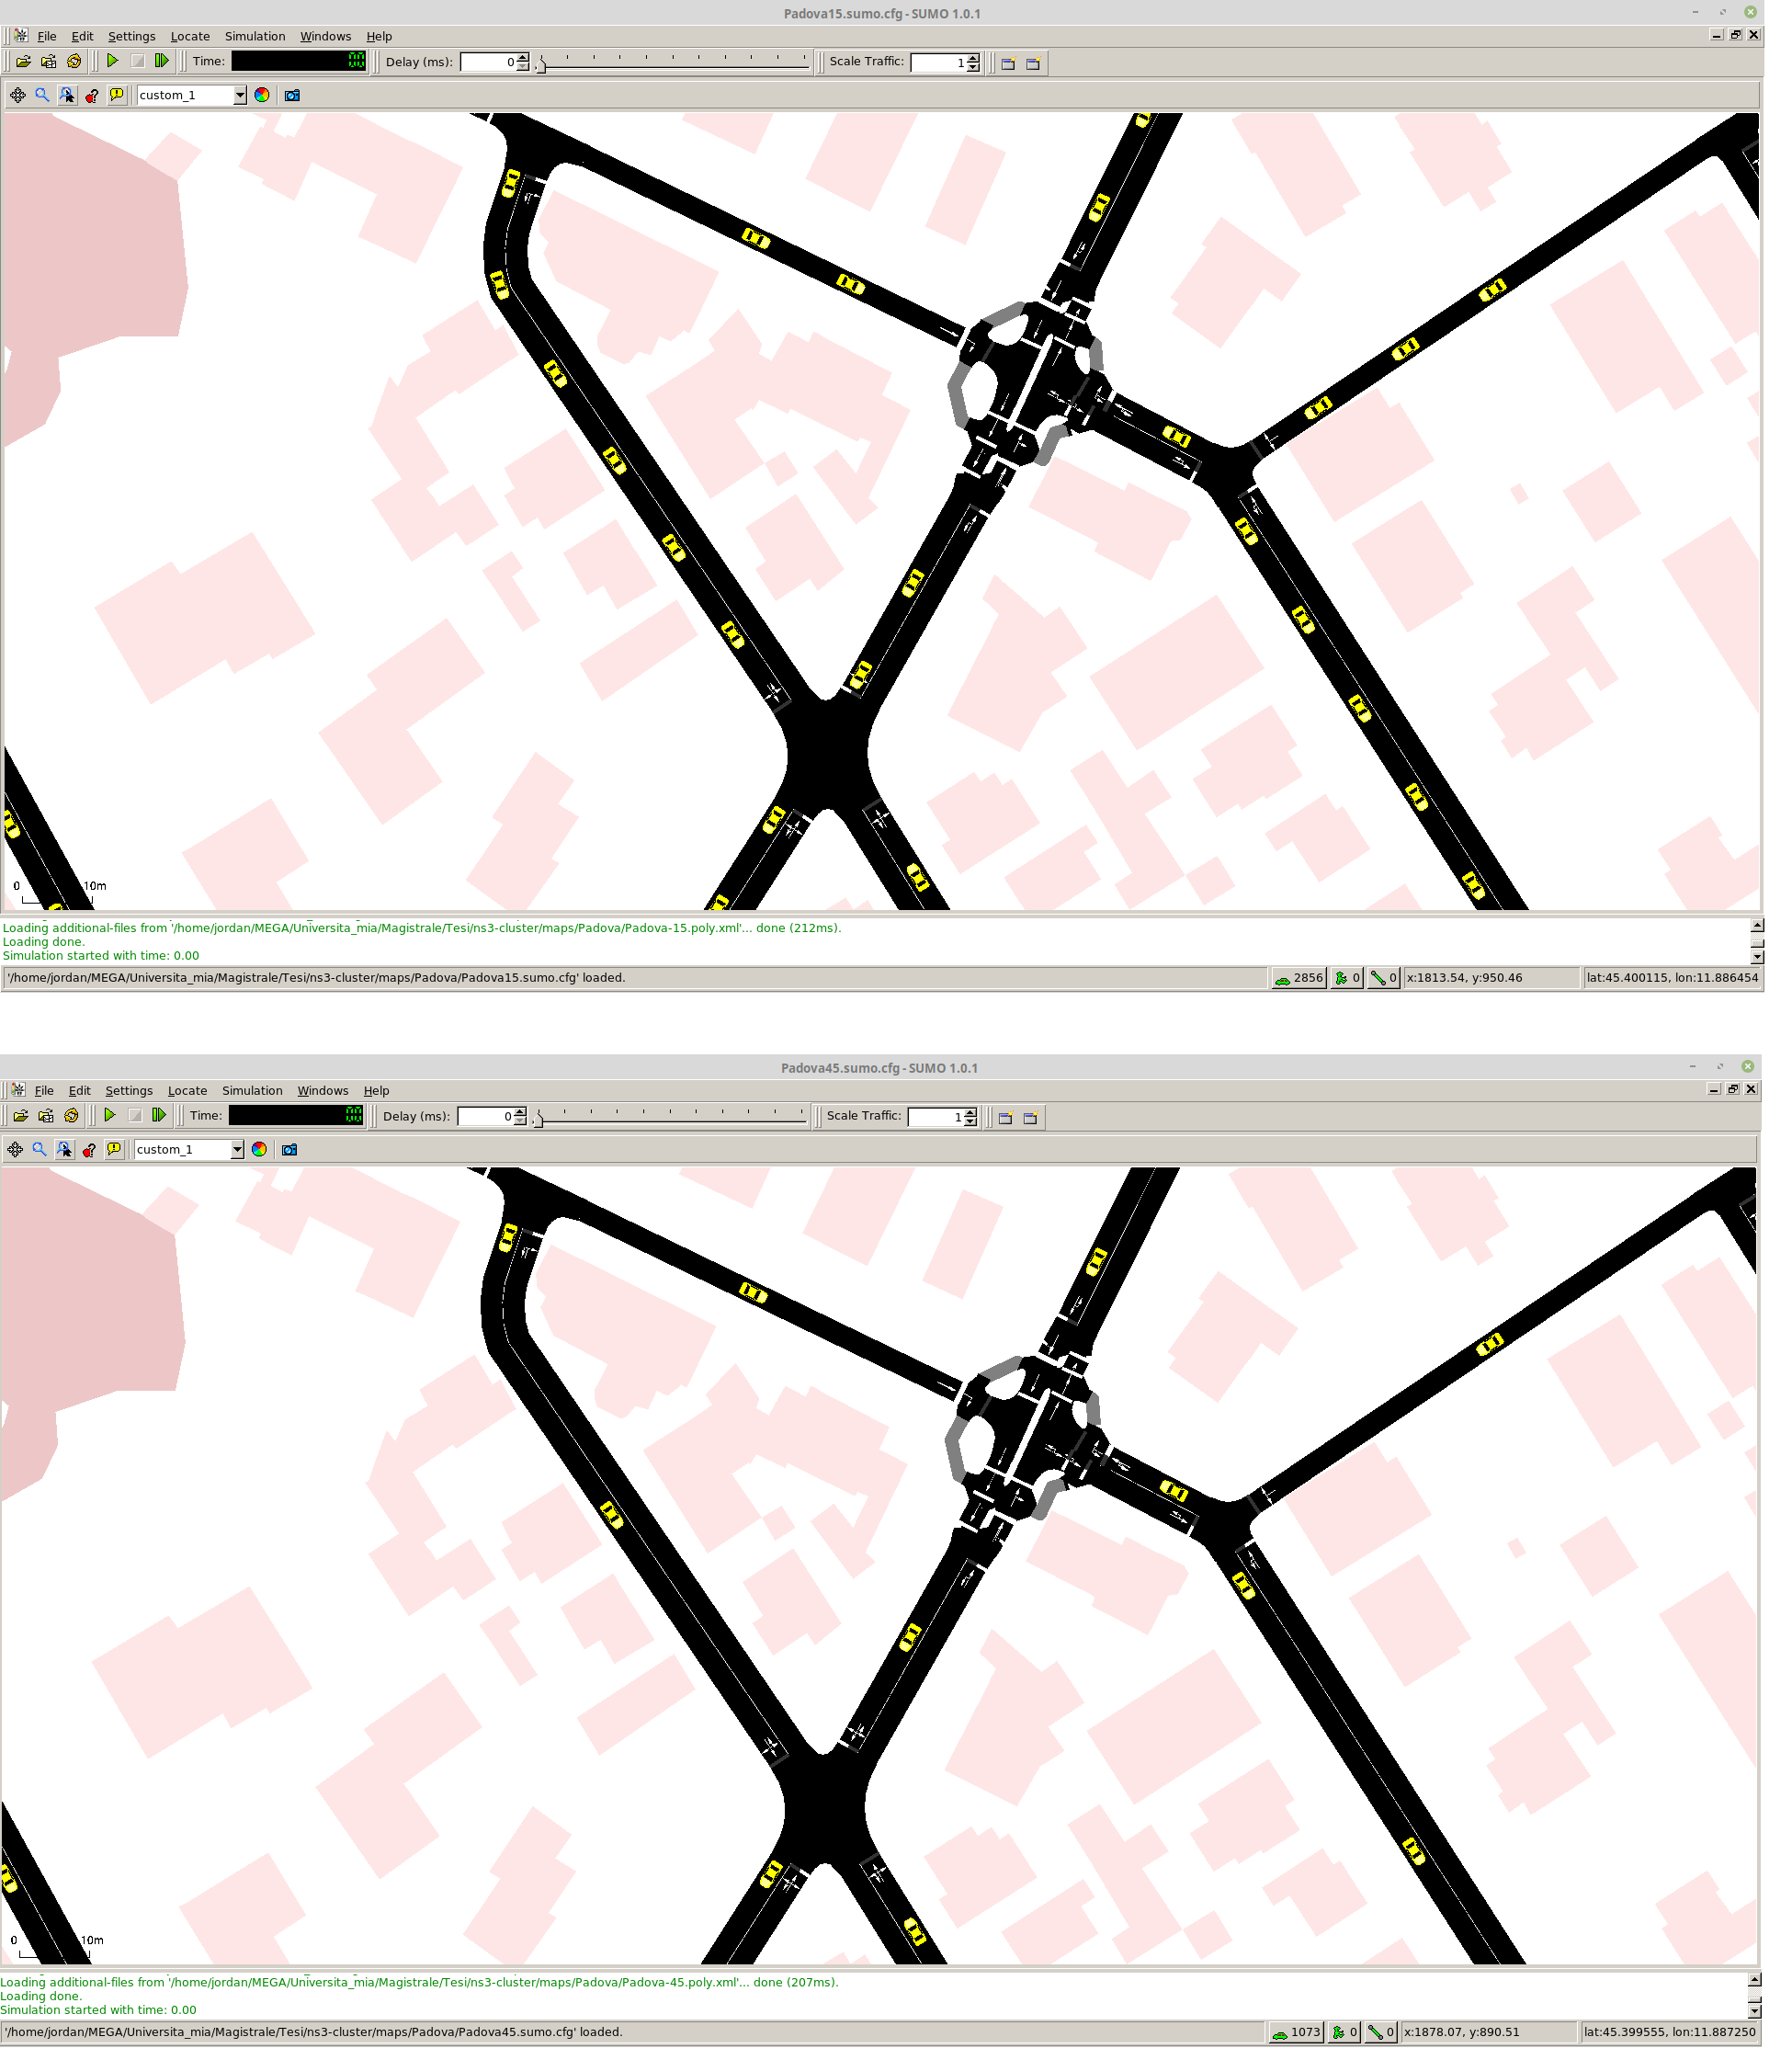
\includegraphics[width=\textwidth]{immagini/sumo-distances}
			\caption{Padua scenario with vehicle distance equals to 15 meters (top) and 45 meters (bottom)}
			\label{fig:sumo-distances}
		\end{figure}
            
% !TEX encoding = UTF-8
% !TEX TS-program = pdflatex
% !TEX root = ../tesi.tex


\chapter{Simulations}
	\label{chapter:simulations}
	After the protocols under consideration have been presented in Chapters \ref{chapter:fb} and \ref{chapter:roff}, this Chapter will contain the results of the simulation carried out through various scenarios of increasing complexity. Several algorithms will be tested, namely:
	\begin{itemize}
		\item Fast-Broadcast and SJ-Fast-Broadcast;
		\item ROFF and SJ-ROFF;
		\item STATIC variants of Fast-Broadcast (e.g. STATIC-100), which behave like Fast-Broadcast but do not employ a transmission range estimation. The only use a static parameter (for example 100 meters for STATIC-100) and use it in the Broadcast Phase;
		\item SJ-STATIC variants of Fast-Broadcast, which also considers junctions during message propagation.
	\end{itemize}
	
	
	Numeric results in every chart will be coupled with their 95\% confidence interval. All following simulation have been run on the High Performance Computing platform of the University of Padua, Department of Mathematics\cite{cluster}.
	
	\section{Metrics}
		\label{sec:metrics}
		Before proceeding with the presentation of simulation results, the metrics used to evaluate the protocols' performances will be presented in this section. 
		
		\subsection{Total Delivery Ratio (TDR)}
			\label{ssec:tdr}
			This metric is used to detect how many vehicles have received the Alert Message in total. Ideally, broadcasting protocols should be able to reach all the reachable nodes in the scenario in order to warn them of the danger. The metric is calculated as follows:
			
			\begin{gather}
				\label{eq:tdr}
				\textit{TDR} = \frac{\textrm{\textit{no. of vehicles successfully receiving the Alert Message}}}{\textrm{\textit{no. of vehicles in the scenario}}}
			\end{gather}
			
			All scenarios are created in a way such that every node can be reached by multi-hop propagation regardless of the source of the Alert Message. In other words, from graph theory point of view, the graph resulting from vehicle distribution where two nodes are connected only if they are within transmission range of each other is a connected graph. This way, the term at the denominator of Equation \ref{eq:tdr} is equivalent to the number of vehicles reachable by pure flooding.
			
		\subsection{Total Delivery Ratio On Circumference (TDROC)}
			This metric is used to detect how many vehicles on the circumference (i.e. the area of interest where the alert data has to be delivered) have received the Alert Message. The circumference is built starting from the source of the Alert Message. The way it is built depends on scenario topology (e.g. 1D, 2D, etc) and will be explained more thoroughly in the following sections.Basically, this metric considers only vehicles far from the source of the AM, instead of all vehicles as in the previous metric. Hence, this is used to measure how effective the algorithm is at delivering the message far from the origin. The metric is calculated as follows:
			
			\begin{gather}
			 	\label{eq:tdroc}
			 	\textit{TDROC} = \frac{\textrm{\textit{no. of vehicles on circ. successfully receiving the Alert Message}}}{\textrm{\textit{no. of vehicles on circ.}}}
			\end{gather}
		
			The same consideration about vehicles and reachability by pure flooding presented in Section \ref{ssec:tdr} is also valid for Equation \ref{eq:tdroc}.
			
		\subsection{Number Of Hops (NOH)}
			This metric is used to measure the mean number of hops required in order to propagate the Alert Message from the source to all vehicles reached on the circumference. This value is obviously dependent on the paths taken by forwarded Alert Messages from the source to all destinations. We have that \textit{NOH} is always greater than or equal to the \textit{Optimal Number of Hops ONOH} (i.e. $ONOH \leq NOH$). \textit{NOH} is calculated using the following formula:
			$$ ONOH = \frac{\textrm{\textit{Circumference Radius}}}{\textrm{\textit{Transmission Range}}} $$
			
			The Number Of Hops metric can be calculated as follows:
			
			\begin{gather}
				\label{eq:noh}
				\textit{NOH} = \frac{ \sum_{p \in RC } \textrm{\textit{no. of hops from source to p}}} {\textrm{|\textit{RC}|}}
			\end{gather}
			
			where $RC$ is the set of vehicles which have successfully received the message on the circumference.
			
			
			The \textit{NOH} metric (whose value should be as close as possible to \textit{ONOH}) is an important indicator of the effectiveness of the multi-hop protocol in choosing the farthest forwarder during contention.
			
			
			Figure \ref{fig:hops} can be used as an example to calculate \textit{NOH}. Using Equation \ref{eq:noh}, the mean number of hops is equal to 3.
			
			\begin{figure}[H]
				\centering
				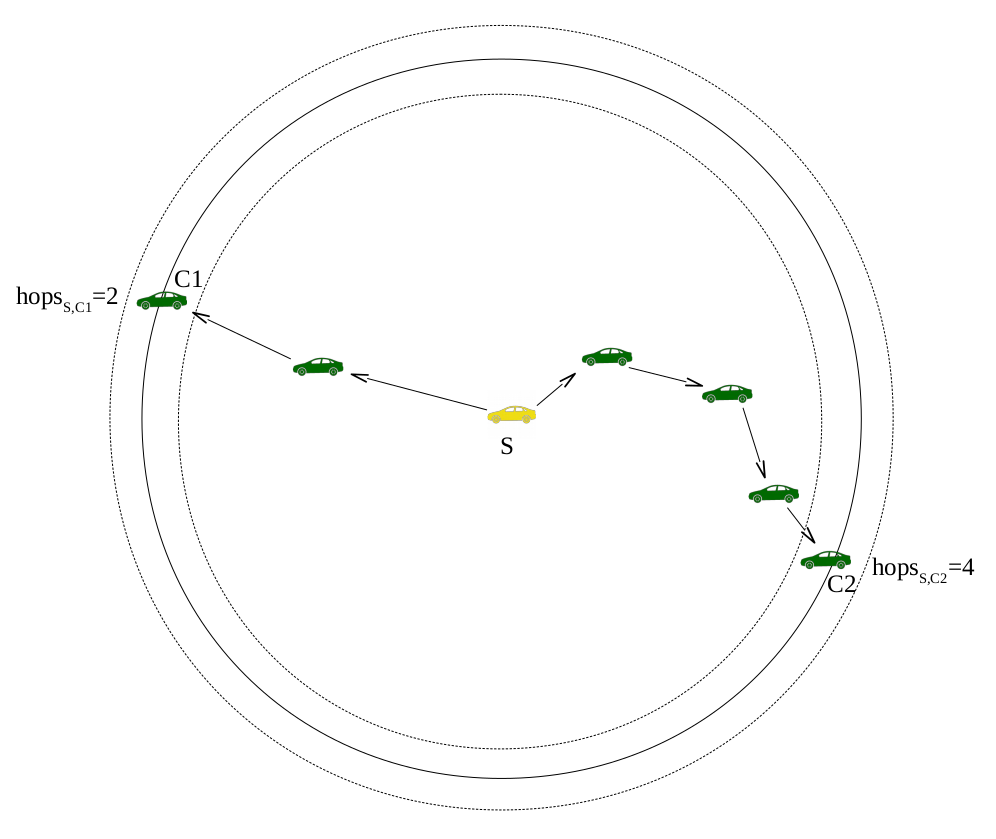
\includegraphics[width=0.7\textwidth]{immagini/hops}
				\caption{Example of \textit{NOH} calculation with Alert Message starting from node S}
				\label{fig:hops}
			\end{figure}
			
		\subsection{Number Of Slots (NOS)}
			This metric is used to measure the number of slots required in order to propagate the Alert Message from the source to all vehicles reached on the circumference. High values of this metric means that the multi-hop protocol introduces a lot of waiting time before each forwarding, hence increasing end-to-end delay and hurting the timeliness of the emergency message propagation.
		
			\begin{gather}
				\label{eq:slots}
				\textit{NOS} = \frac{ \sum_{p \in RC } \textrm{\textit{no. of slots waited along path from source to p}}}  {\textrm{|\textit{RC}|}}
			\end{gather}	
	
			where $RC$ is the set of vehicles which have successfully received the message on the circumference.
			The number of slots along the path from node $a$ to $b$ at the numerator of Equation \ref{eq:slots} is the sum of the slots waited by each forwarder before relaying the Alert Message. 
			
			
			Based on the scenario represented in Figure \ref{fig:slots} and Equation \ref{eq:slots}, the mean number of slots from source S to nodes on the circumference is 100.
			
			\begin{figure}[H]
				\centering
				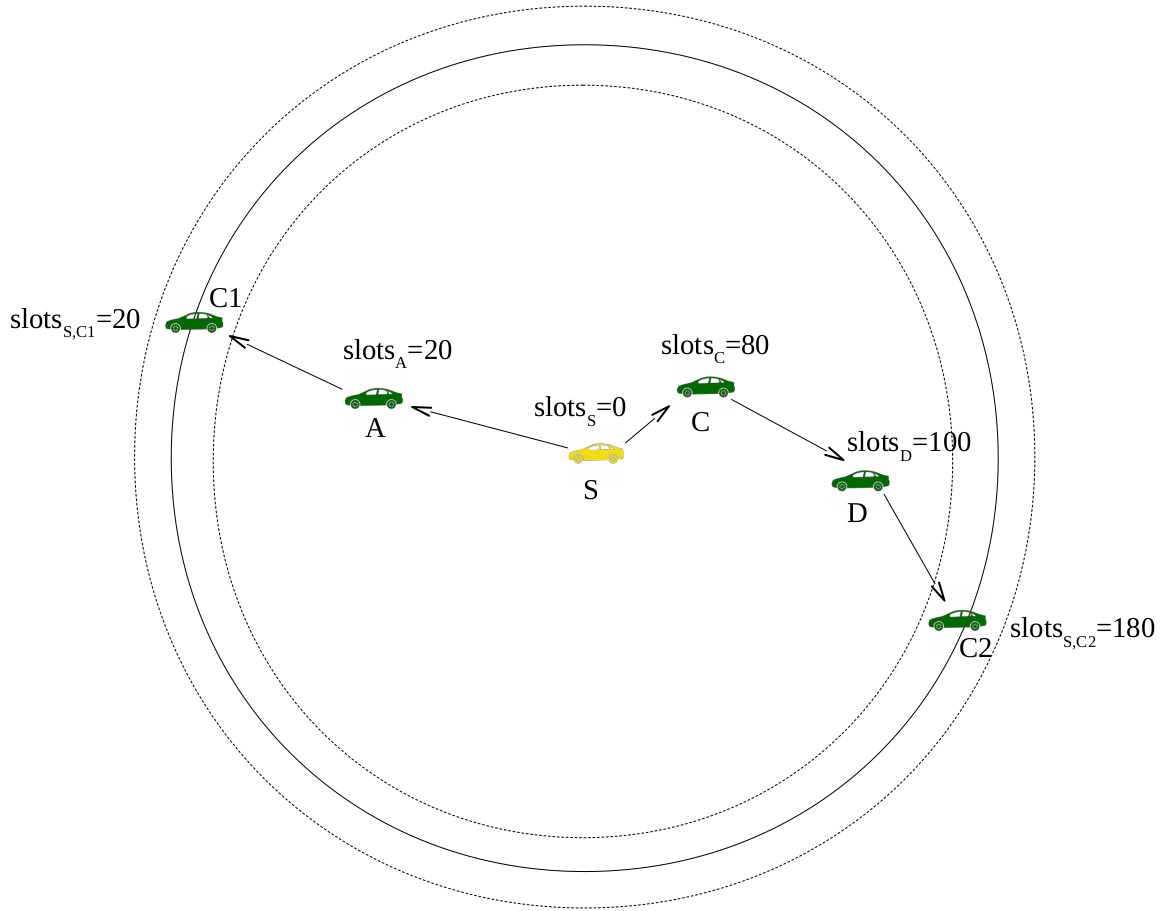
\includegraphics[width=0.7\textwidth]{immagini/slots}
				\caption{Example of \textit{NOS} calculation with Alert Message starting from node S}
				\label{fig:slots}
			\end{figure}
			
			
		\subsection{Forwarding Node Number (FNN)}
			This metric is used to measure the number of vehicles which forward the Alert Message. The value of this metric is an indicator of the effectiveness of the multi-hop protocol in successfully suppressing scheduled transmissions from \acrshort{pfca}s after the \acrshort{ffca} has relayed the message. The metric is calculated as follows:
			 
			\begin{gather}
				\label{eq:nos}
				\textit{FNN} = \textrm{\textit{no. of vehicles forwarding the Alert Message}}
			\end{gather}	
				
	\section{Platoon scenario}
		The first scenario taken into consideration is a simple one-dimensional platoon scenario, where vehicles are placed in a strip-like area 15 kilometers long. Vehicles are 25 meters distant from each other. Transmission ranges of 100, 300 and 500 has been employed during simulations. 
		Parameters for this scenario are included in Table \ref{table:platoon}.  These parameters will also be true for all following scenarios, unless specified otherwise.
		
		\begin{table}[H]
			\def\arraystretch{1.1}
			\rowcolors{2}{D}{P}	
			\begin{tabularx}{\textwidth}{l | l  l}
				\rowcolor{I} {\large \textcolor{white}{Parameter}} & {\large \textcolor{white}{Value}} & {\large \textcolor{white}{}} \TBstrut  \\
				\toprule
				\endhead
	%			\midrule[1pt]
				\rowcolor{P} \multicolumn{3}{c}{Scenario configuration} \\
				\midrule[1pt]
				Road length 							& 15000 				& m		\\
				Distance between vehicles 				& 25					& m		\\
				Circumference	radius					& 14000					& m		\\
				Number of vehicles						& 600					& 		\\
				Source of alert message position		& Left of platoon		&		\\
				\midrule[1pt]
				\rowcolor{P} \multicolumn{3}{c}{Network configuration} \\
				\midrule[1pt]
				Packet payload size						& 100					& byte	\\	
				Transmission standard					& 802.11b				&		\\
				Frequency								& 2.4					& GHz	\\
				Channel bandwidth						& 22					& MHz	\\
				Transmission speed						& 11					& Mbps	\\
				Transmission powers						& -7.0, 4.6, 13.4		& dBm	\\
				Transmission range						& 100, 300, 500			& m		\\
				Modulation								& DSSS					& 		\\
				Mobility model							& ns3::ConstantPosition	&		\\
				Propagation loss model					& ns3::TwoRayGround 	&		\\
				Propagation delay model					& ns3::ConstantSpeed	&		\\
				Shadowing model							& No					&		\\
				Junction modeling						& No					&		\\
				\midrule[1pt]
				\rowcolor{P} \multicolumn{3}{c}{Protocols configuration} \\
				\midrule[1pt]
	%			Protocols tested						& \makecell{FB, ROFF, STATIC100, \\ STATIC300, STATIC500} & \\
				FB contention window					& [32, 1024]			& slot	\\
				ROFF distance range (\textit{k} parameter) & 1					&		\\	
				\midrule[1pt]
				Number of simulations per configuration	& 1000					&		\\
				\bottomrule
			\end{tabularx}
			\caption{Platoon scenario configuration}
			\label{table:platoon}
		\end{table}
	
		\begin{figure}[H]
			\centering
			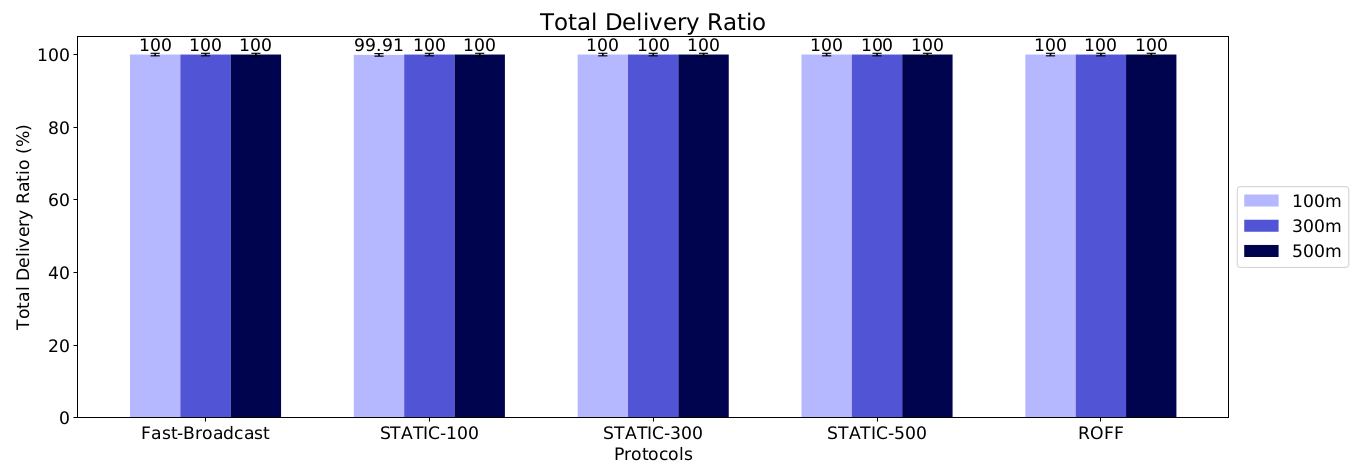
\includegraphics[width=1.1\textwidth]{immagini/platoon-15km/tdr}
			\caption{\textit{TDR} metric for Platoon scenario}
			\label{fig:metric-platoon-15km-0}
		\end{figure}
	
		\begin{figure}[H]
			\centering
			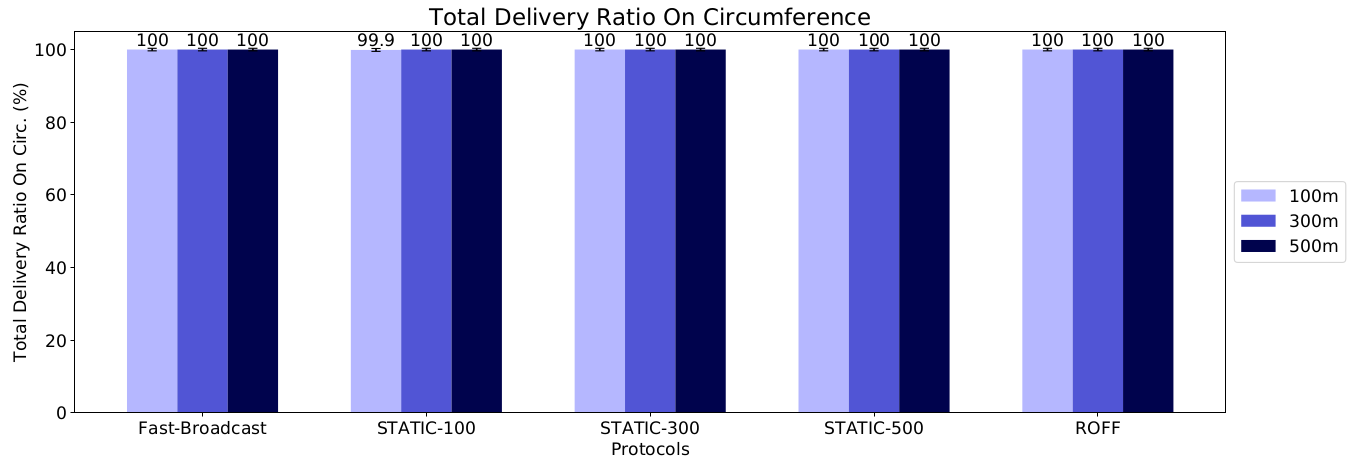
\includegraphics[width=1.1\textwidth]{immagini/platoon-15km/tdroc}
			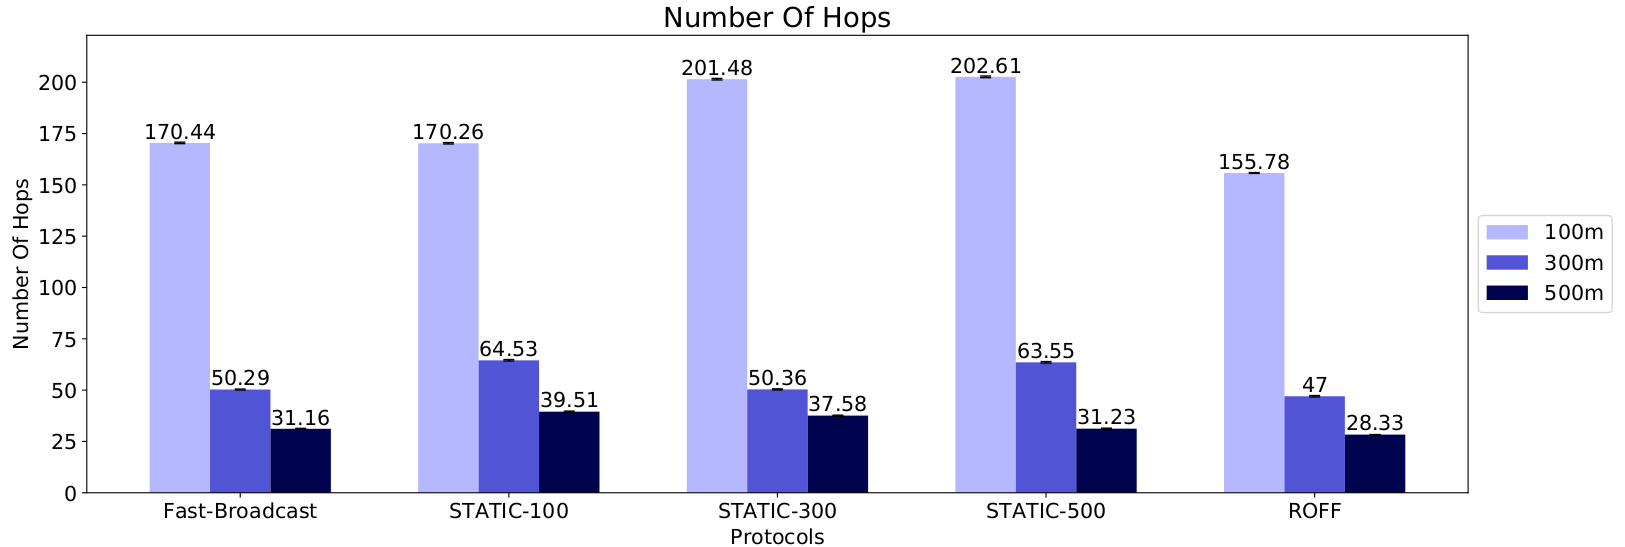
\includegraphics[width=1.1\textwidth]{immagini/platoon-15km/noh}
			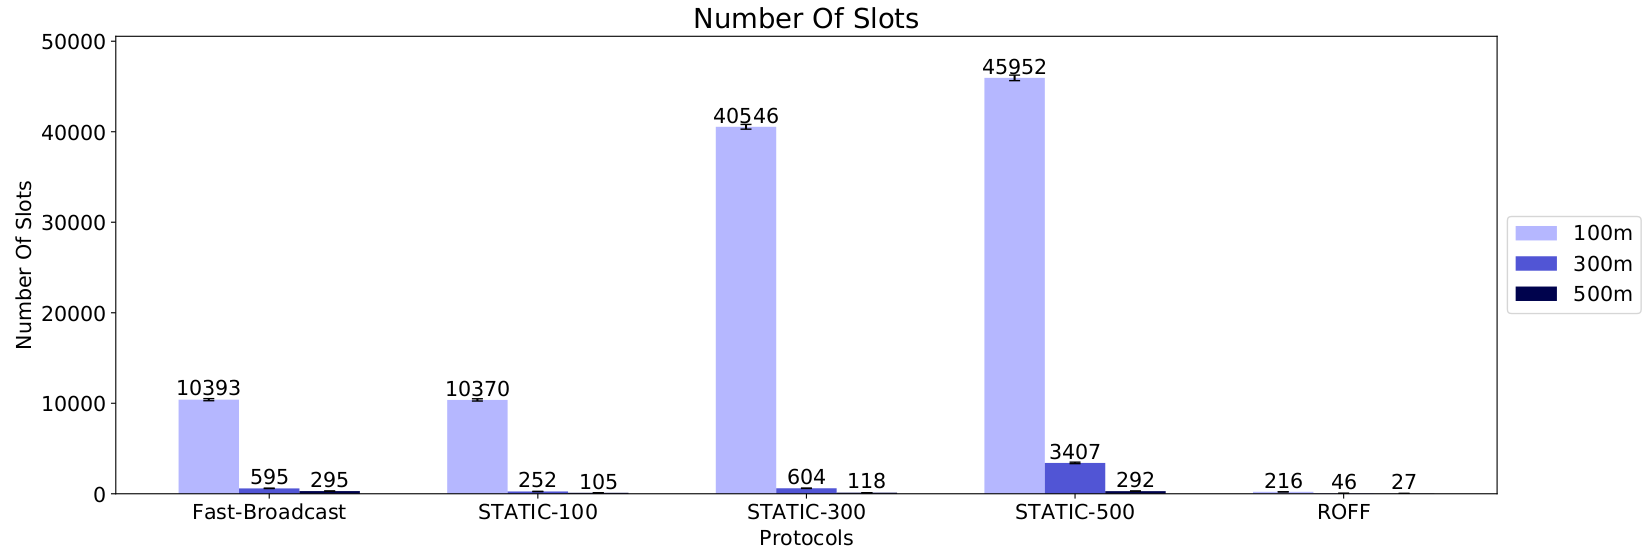
\includegraphics[width=1.1\textwidth]{immagini/platoon-15km/nos}
			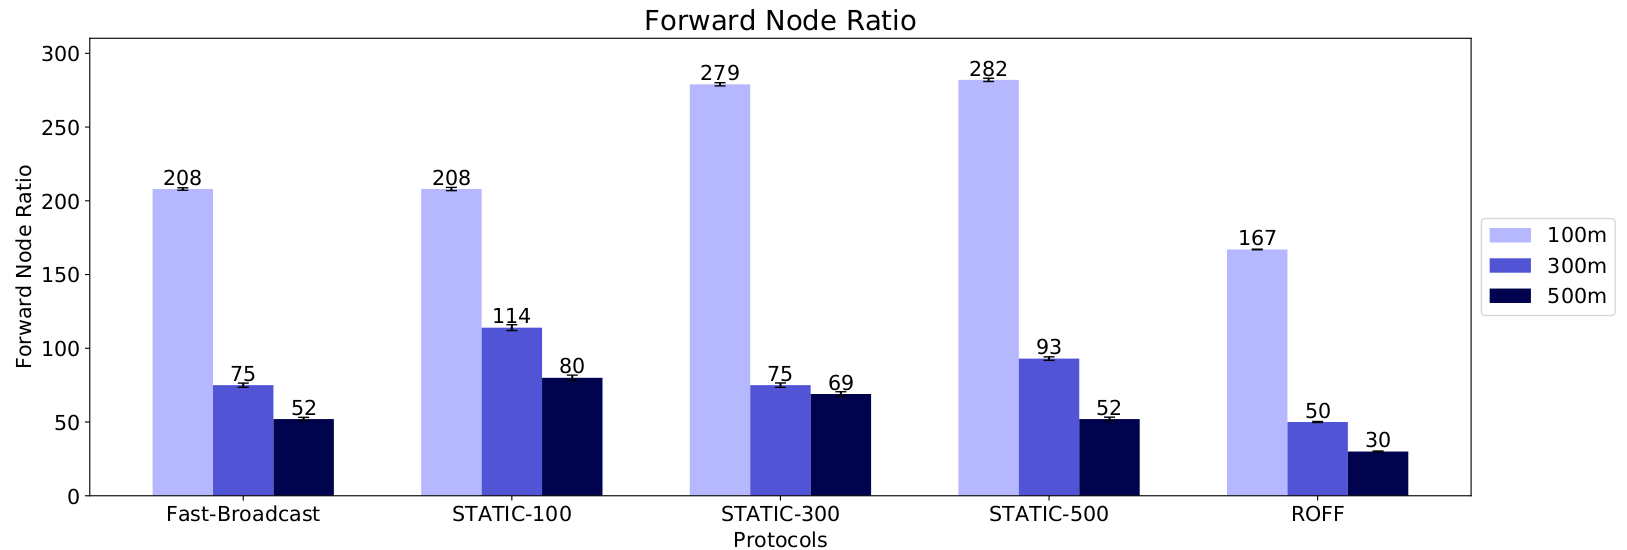
\includegraphics[width=1.1\textwidth]{immagini/platoon-15km/fnn}
			\caption{\textit{TDROC}, \textit{NOH}, \textit{NOS} and \textit{FNN} metrics for Platoon scenario}
			\label{fig:metric-platoon-15km-1}
		\end{figure}
	
		\newpage
	
		Since this scenario is one-dimensional, the circumference simply consists in vehicles distant $14.000  \pm 25$ meters from the source of Alert Message. Both metrics about delivery ratios (global and on circumference) are exactly 100\%, so the algorithms successfully propagate the \acrshort{ama} until the end of the platoon.
		
		
		Considering the Number Of Hops, ROFF's results are 11.76\%, 6.54\% and 9.08\% lower than Fast-Broadcast's results respectively for 100, 300 and 500 meters transmission range. ROFF's results are close to the optimal number of hops, respectively 140, 46.6 and 28 for the same transmission ranges as above. This means that the forwarder selection algorithms based on ESD Bitmap works better at choosing the farthest vehicle from the previous forwarder compared to the contention window approach for 1D scenarios. Considering STATIC variants of Fast-Broadcast, it is possible to observe that the STATIC-tx variant produces comparable results with Fast-Broadcast with \textit{tx} transmission range (e.g. STATIC-100 value is comparable to Fast-Broadcast with 100 meters transmission range), as expected. The STATIC protocol performs worse (hence the Number of Hops increases) whenever the transmission range is underestimated (e.g. STATIC-100 with 300 meters transmission range, compared to Fast-Broadcast with the same transmission range) or overestimated (e.g. STATIC-500 with 100 meters transmission range, compared to Fast-Broadcast with the same transmission range). This behaviour is expected, as reported in \cite{BAR2017}.
		
		
		Regarding the Number of Slots, ROFF performs much better than Fast-Broadcast. The metric's value is decreased respectively by 97.92\%, 92.27\% and 90.85\% using ROFF. The waiting time calculation, based on unique forwarding priority instead of distance, guarantees a much lower wait compared to Fast-Broadcast contention window approach. As before, STATIC approaches produce results comparable with Fast-Broadcast when the transmission range estimation is correct. Instead, the Number of Slots greatly increases when the transmission range is underestimated and decreases when the transmission range is overestimated. In this last case, the decrease in \textit{NOS} comes with an increase in Number Of Hops reported in the previous paragraph, so an overestimation of transmission range is not desirable.
		
		
		Lastly, it is possible to see that ROFF achieves a better suppression of redundant transmissions, guaranteeing a decrease of 19.71\%, 33.33\% and 42.31\% respectively for each one of the transmission ranges considered.
		
		
	\section{Grid scenario}
		\label{sec:grid}
		After tests on the 1D Platoon scenario have been carried out, the next step consisted in testing the algorithms' performances in a two-dimensional Grid scenario, employing also the shadowing model introduced in \ref{sec:shadowing}. The Grid scenario consisted in a grid built by 17 north-south and 17 west-east roads, distant 300 meters from each other. Each road is 10 meters wide. Vehicles are placed only inside roads and are 25 meters distant from each other. The source of the Alert Message is in the middle of the grid, and the circumference has a radius of 2000 meters. For metrics calculation, vehicles are considered inside the circumference if they are $2000 \pm 25$ meters far from the source. Buildings are placed inside the blocks generated by road intersections, and are square shaped with an edge of 290 meters.
		
		
		Parameters for this scenario are included in Table \ref{tab:grid}.  
		
		\begin{table}[H]
			\def\arraystretch{1.1}
			\rowcolors{2}{D}{P}	
			\begin{tabularx}{\textwidth}{l | l  l}
				\rowcolor{I} {\large \textcolor{white}{Parameter}} & {\large \textcolor{white}{Value}} & {\large \textcolor{white}{}} \TBstrut  \\
				\toprule
				\endhead
				%			\midrule[1pt]
				\rowcolor{P} \multicolumn{3}{c}{Scenario configuration} \\
				\midrule[1pt]
				Road length 							& 4800	 				& m		\\
				Distance between roads					& 300					& m		\\
				Road width								& 10					& m		\\
				Number of roads (vertical)				& 17					&		\\
				Number of roads (horizontal)			& 17					&		\\
				Distance between vehicles 				& 25					& m		\\
				Circumference radius					& 2000					& m		\\
				Number of vehicles						& 6528					& 		\\
				Source of alert message position		& Center				&		\\
				Edge of buildings						& 290					& m		\\
				Number of buildings						& 255					& m		\\
				\midrule[1pt]
				\rowcolor{P} \multicolumn{3}{c}{Simulator configuration} \\
				\midrule[1pt]
				Shadowing model							& Obstacle Shadowing	&		\\
				Junction modeling						& No					&		\\
				\midrule[1pt]
				Number of simulations per configuration	& 1000					&		\\
				\bottomrule
			\end{tabularx}
			\caption{Grid scenario configuration}
			\label{tab:grid}
		\end{table}
	
		\begin{figure}[H]
			\centering
			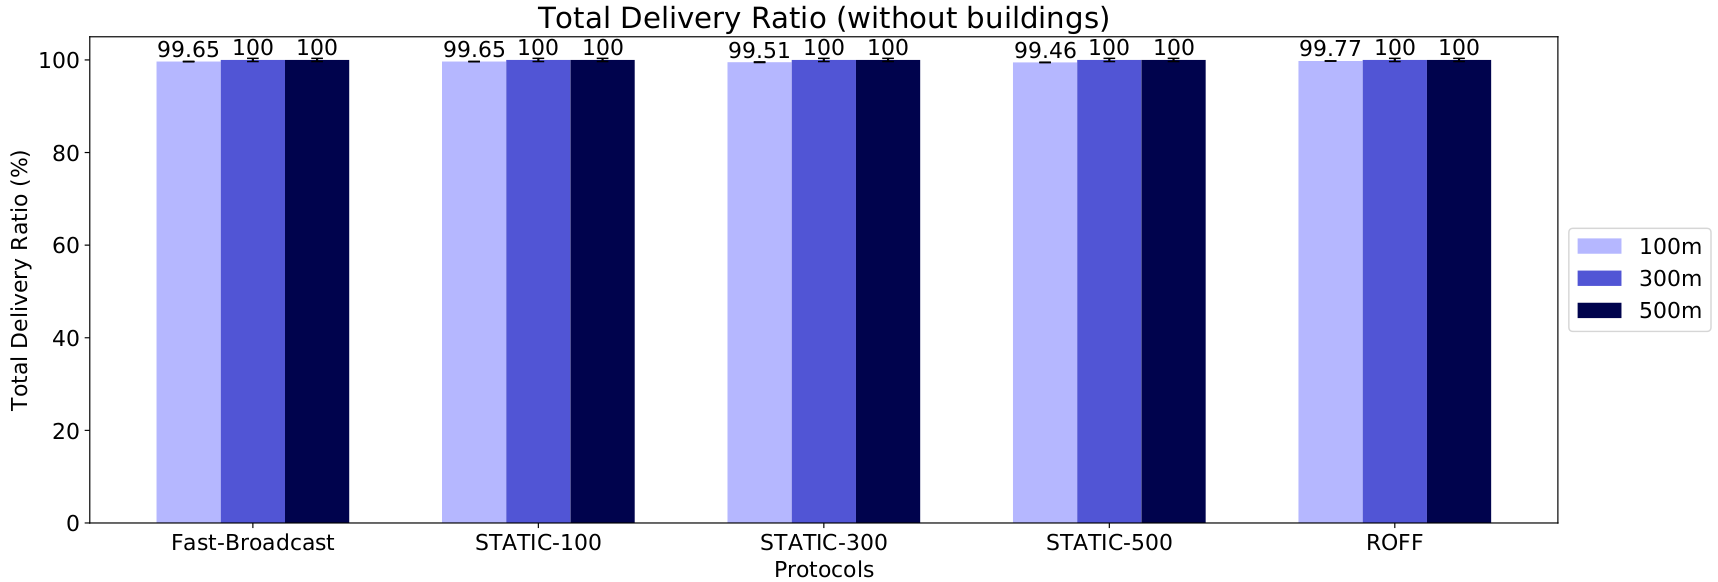
\includegraphics[width=1.0\textwidth]{immagini/grid-300/b0/tdr}
			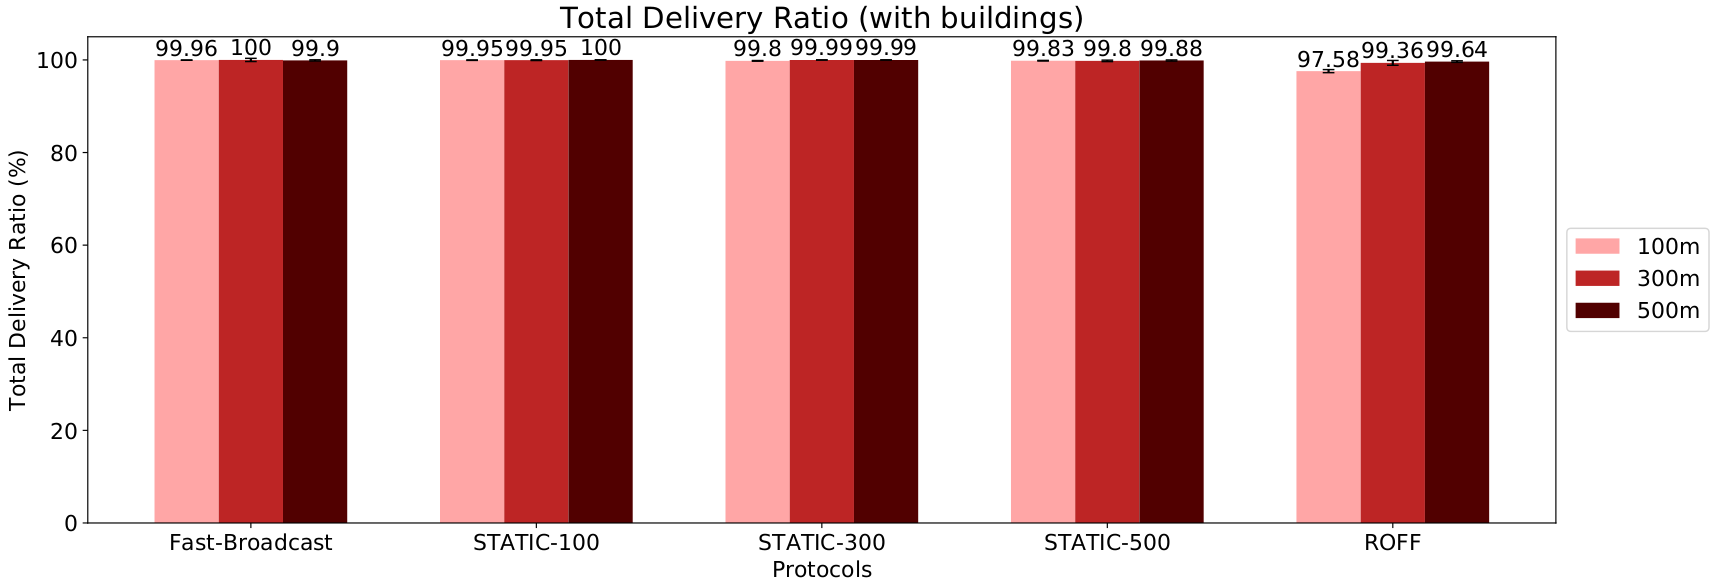
\includegraphics[width=1.0\textwidth]{immagini/grid-300/b1/tdr}
			\caption{\textit{TDR} without buildings (top) and with buildings (bottom) for Grid scenario}
			\label{fig:grid-tdr}
		\end{figure}
		
		\begin{figure}[H]
			\centering
			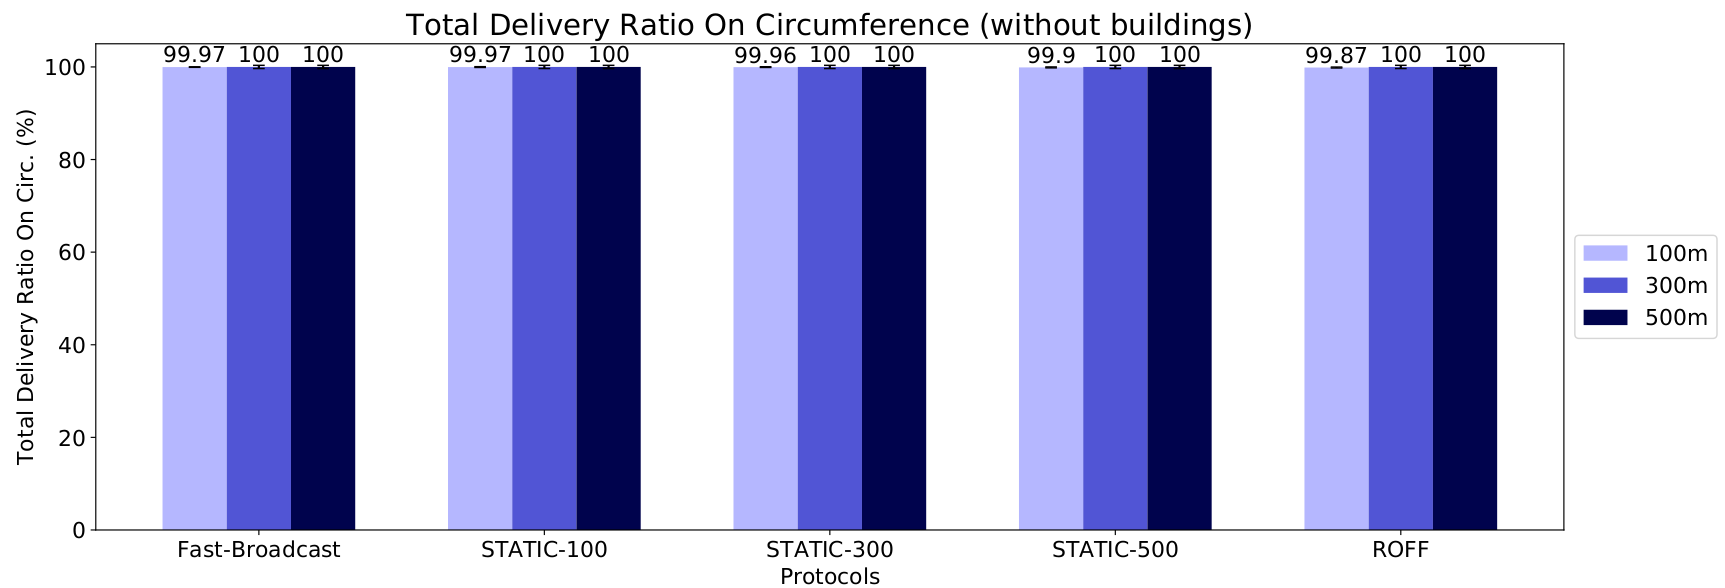
\includegraphics[width=1.0\textwidth]{immagini/grid-300/b0/tdroc}
			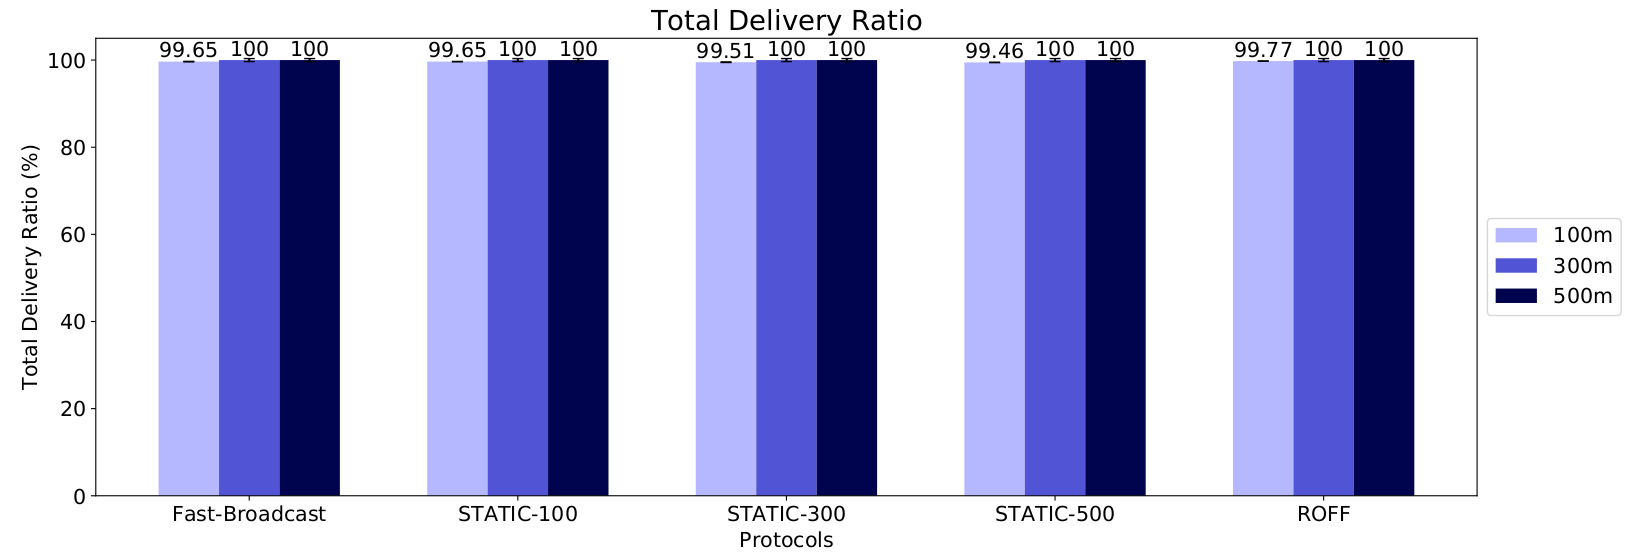
\includegraphics[width=1.0\textwidth]{immagini/grid-300/b1/tdroc}
			\caption{\textit{TDROC} without buildings (top) and with buildings (bottom) for Grid scenario}
			\label{fig:grid-tdroc}
		\end{figure}
	
		\begin{figure}[H]
			\centering
			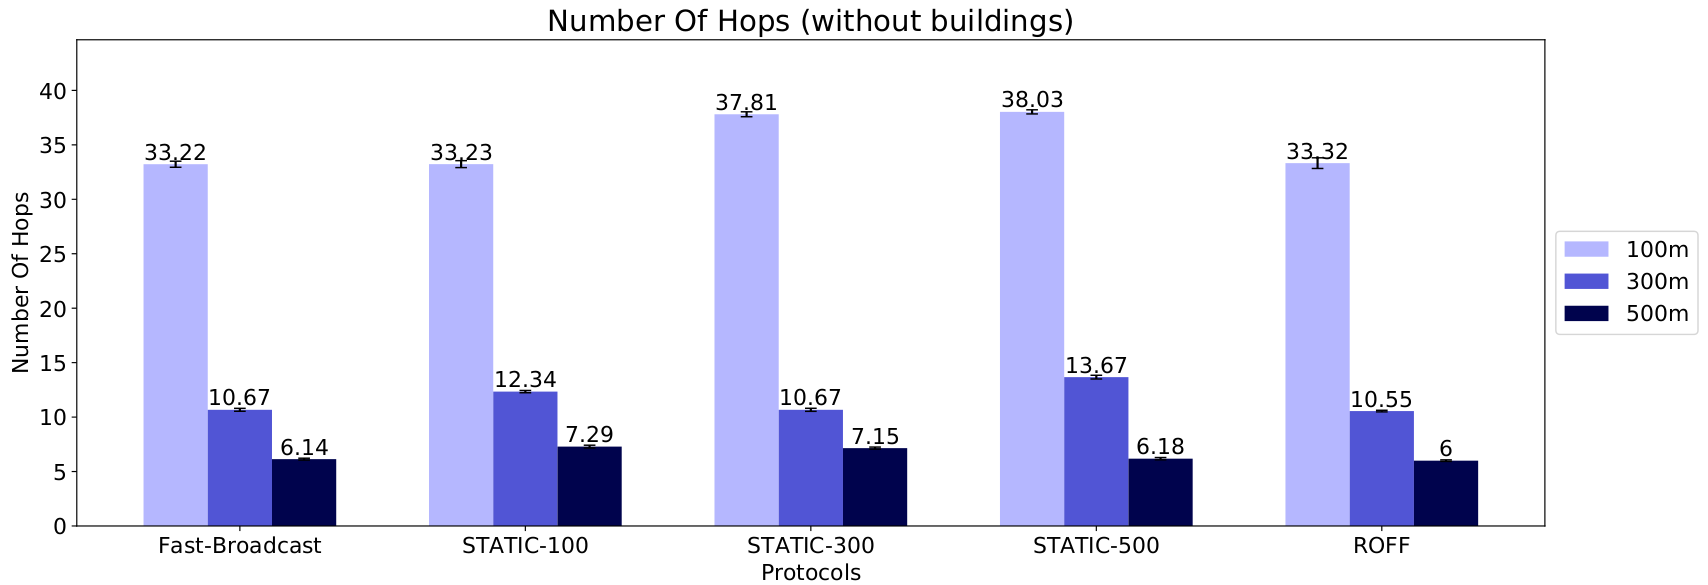
\includegraphics[width=1.0\textwidth]{immagini/grid-300/b0/noh}
			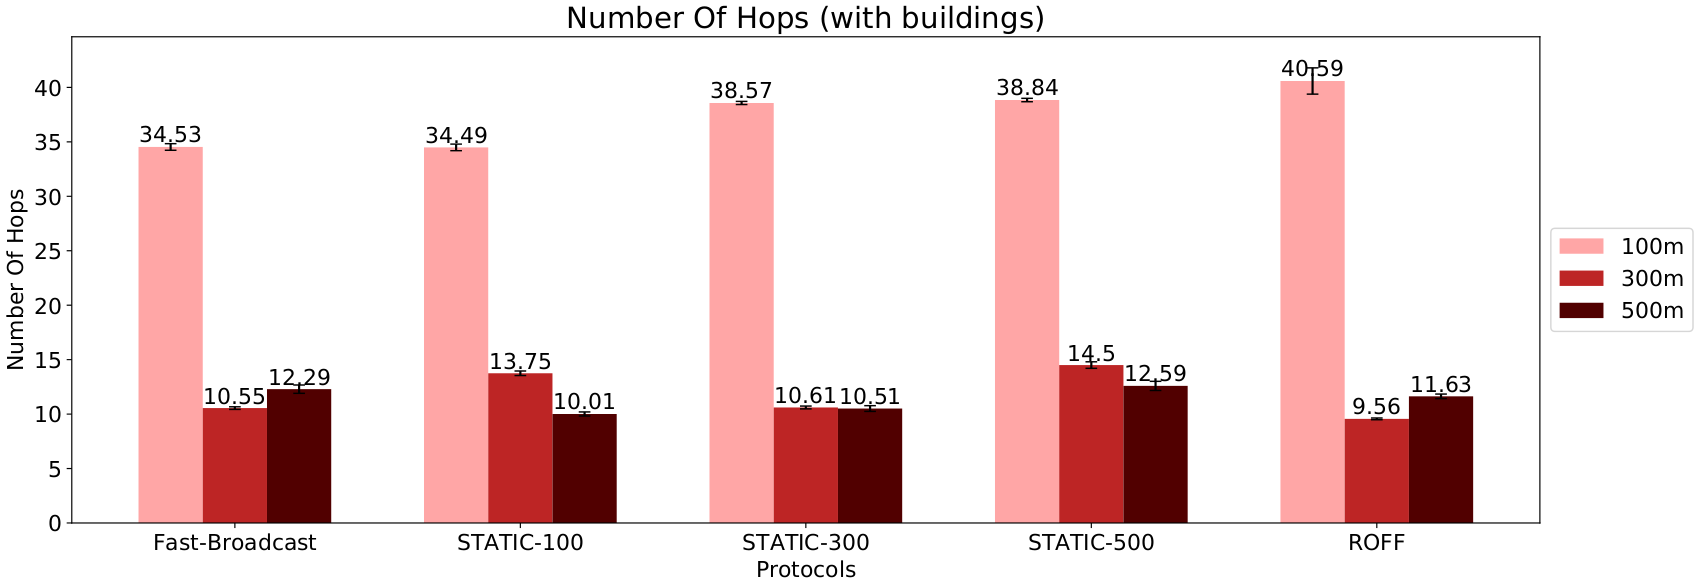
\includegraphics[width=1.0\textwidth]{immagini/grid-300/b1/noh}
			\caption{\textit{NOH} without buildings (top) and with buildings (bottom) for Grid scenario}
			\label{fig:grid-noh}
		\end{figure}
	
		\begin{figure}[H]
			\centering
			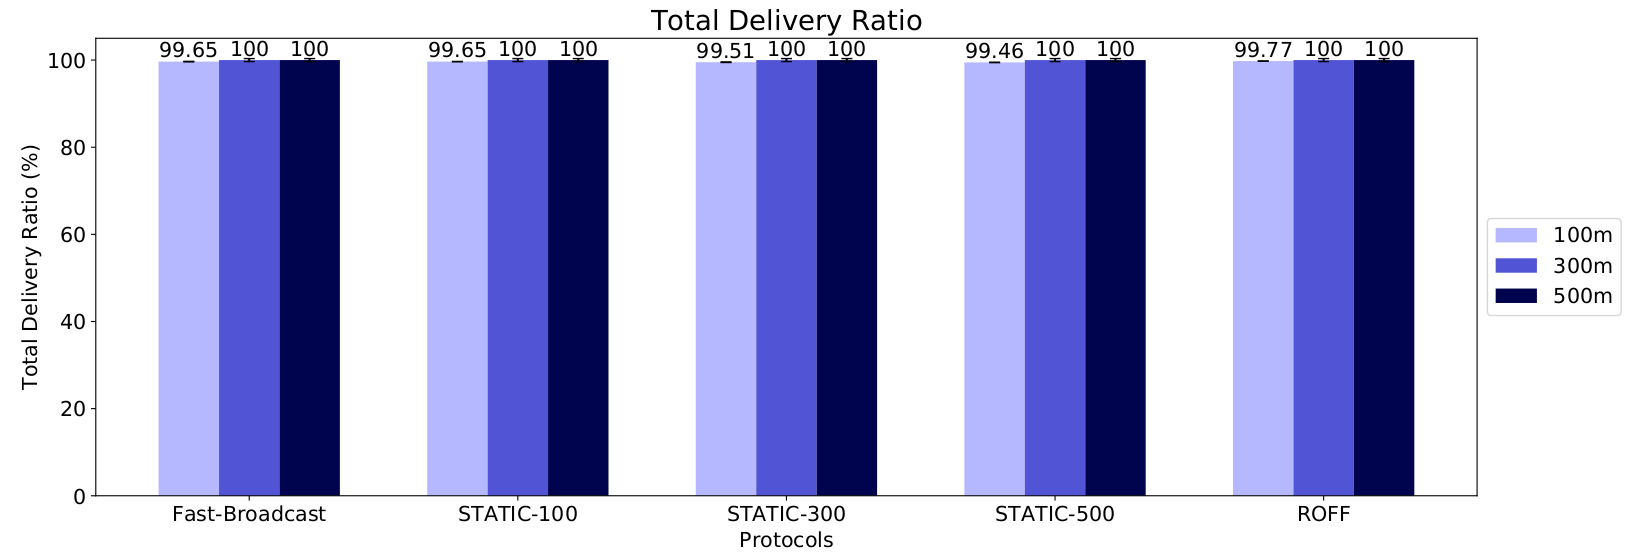
\includegraphics[width=1.0\textwidth]{immagini/grid-300/b0/nos}
			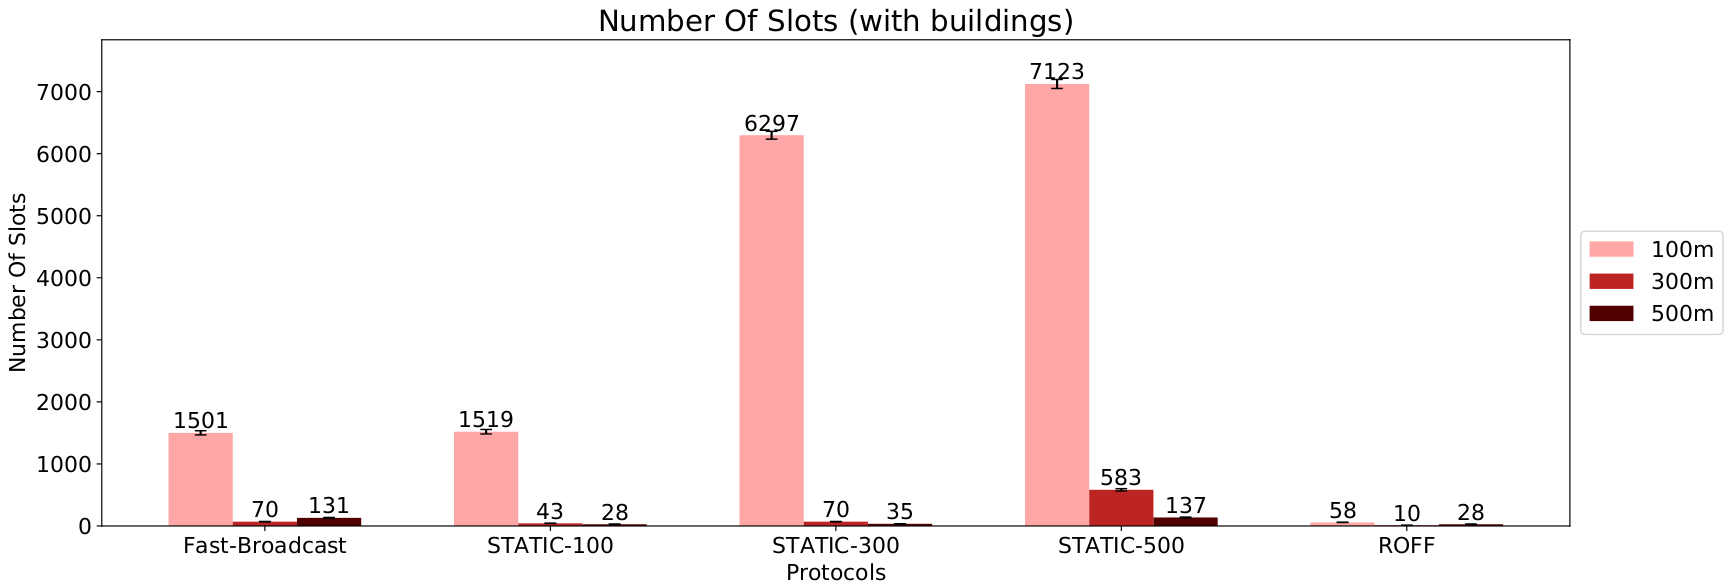
\includegraphics[width=1.0\textwidth]{immagini/grid-300/b1/nos}
			\caption{\textit{NOS} without buildings (top) and with buildings (bottom) for Grid scenario}
			\label{fig:grid-nos}
		\end{figure}
	
		\begin{figure}[H]
			\centering
			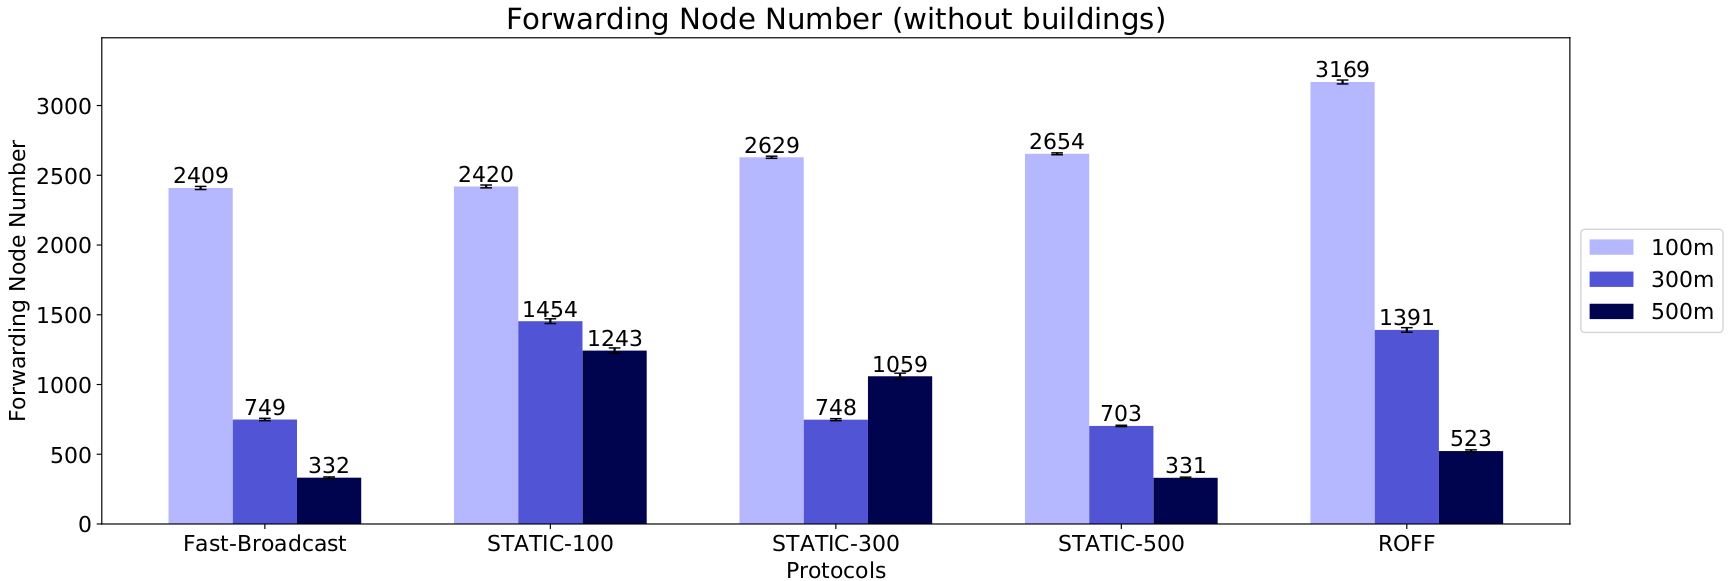
\includegraphics[width=1.0\textwidth]{immagini/grid-300/b0/fnn}
			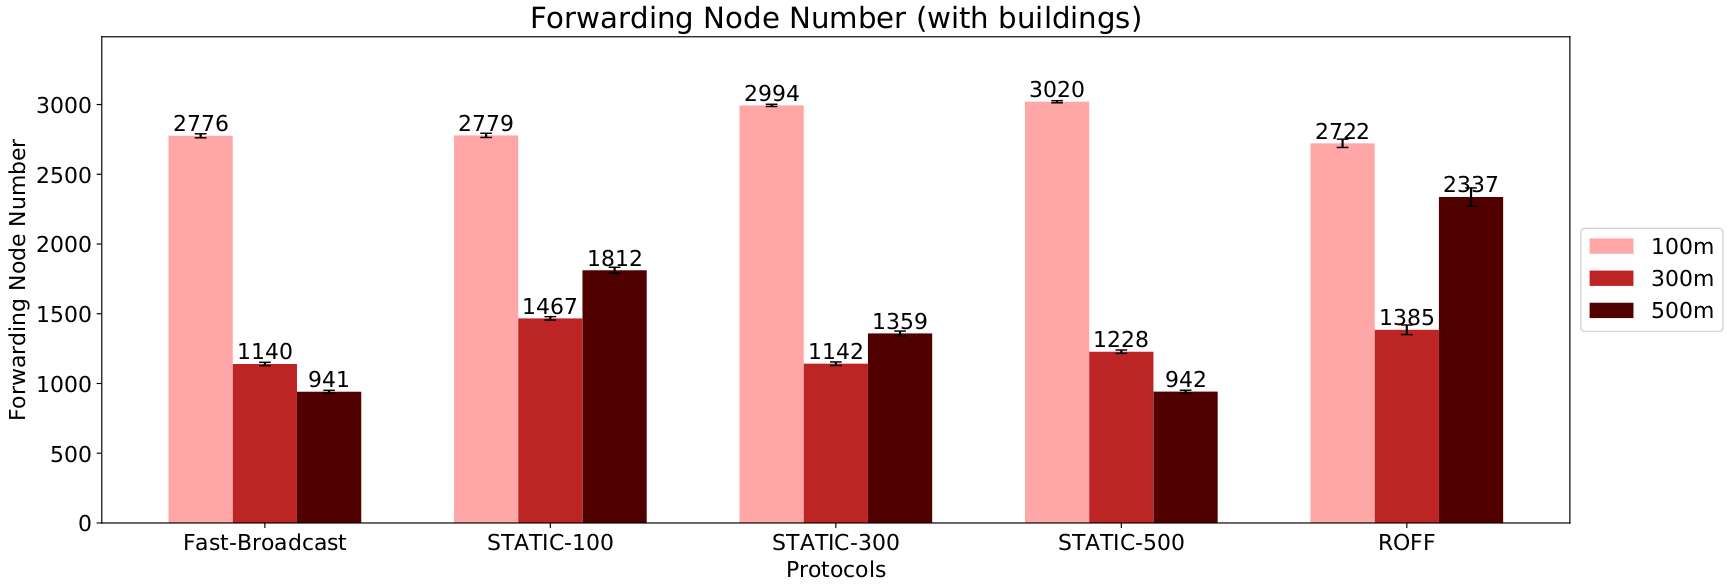
\includegraphics[width=1.0\textwidth]{immagini/grid-300/b1/fnn}
			\caption{\textit{FNN} without buildings (top) and with buildings (bottom) for Grid scenario}
			\label{fig:grid-fnn}
		\end{figure}
		
		\newpage
		
		All the algorithms perform well as far as delivery ratios are concerned (Figure \ref{fig:grid-tdr} \ref{fig:grid-tdroc}), for both configurations with and without buildings. This means that the shadowing caused by the Obstacle Model does not create no-reach zones, and the signal manages to find its way to almost all of the vehicles. The regular pattern by which vehicles are placed may help with that: further testing where this hypothesis is removed will be presented in the next sections. Even though delivery ratios are unchanged, the effect of the Obstacle model can be observed qualitatively comparing Figure \ref{fig:fb-b0-grid-transmission} and \ref{fig:fb-b1-grid-transmission} for Fast-Broadcast, and Figure \ref{fig:roff-b0-grid-transmission} and \ref{fig:roff-b1-grid-transmission} for ROFF. The effects of obstacles on propagation cause the signal to travel only through roads segments where line of sight is possible. Instead, without obstacles the signal can be propagated freely in all directions.
		
		
		Moreover, Fast-Broadcast and ROFF can be compared with each other by looking at Figure \ref{fig:fb-b0-grid-transmission} and \ref{fig:roff-b0-grid-transmission} for the scenario without buildings, and Figure \ref{fig:fb-b1-grid-transmission} and \ref{fig:roff-b1-grid-transmission} for the scenario with buildings. In both cases, ROFF designates the furthest PFC as the next forwarder much more reliably than Fast-Broadcast thanks to the Neighbor Table mechanism. Instead, Fast-Broadcast relies on a random choice of waiting time, so the next designated forwarder is sometimes not one of the farthest vehicles from the previous forwarder. Based on this observation, we can expect a much lower NOH value for ROFF. Quantitative analysis of this and other metrics will be reported in the next paragraphs of this section.
		
		\begin{figure}[H]
			\centering
			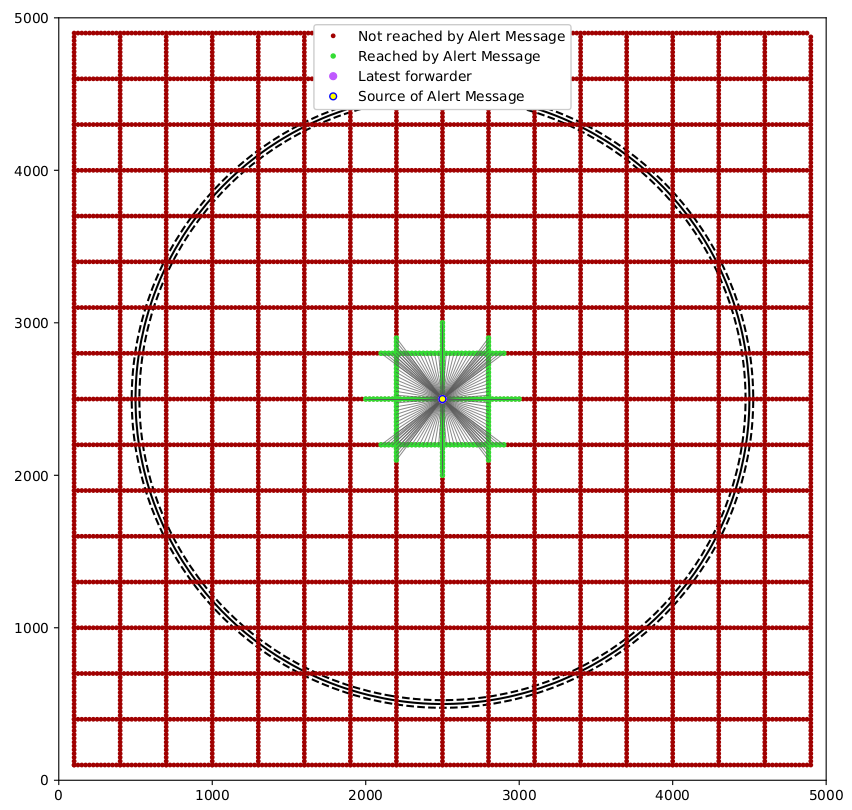
\includegraphics[width=0.8\textwidth]{immagini/grid-300/b0/fb-1hop}
			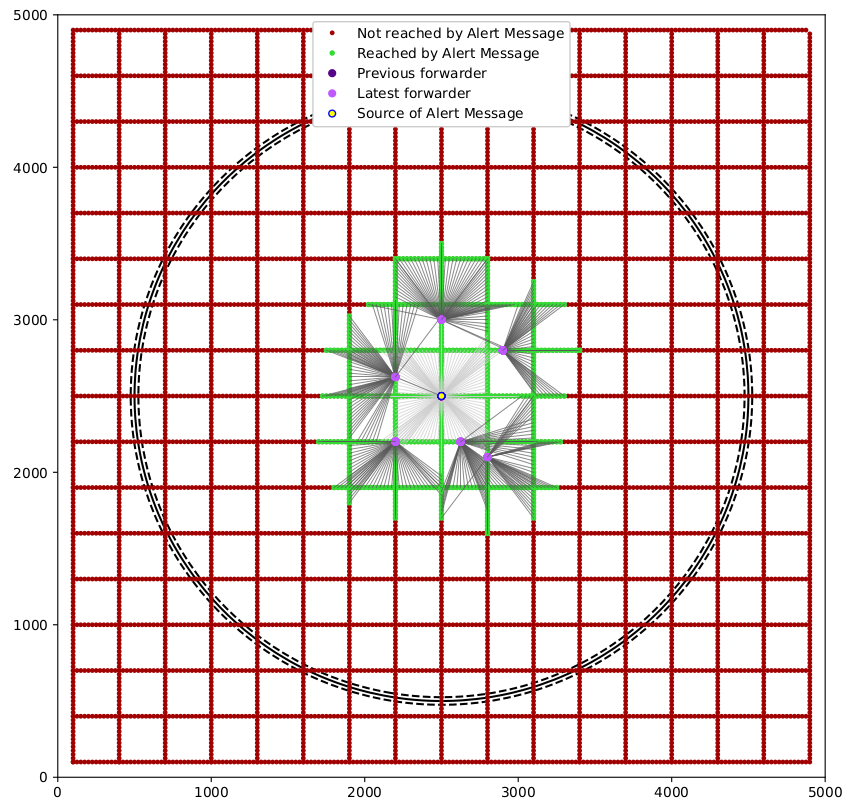
\includegraphics[width=0.8\textwidth]{immagini/grid-300/b0/fb-2hop}
			\caption{Fast-Broadcast after 1 hop (top) and 2 hops (bottom) in Grid scenario with 500 meters transmission range and without the Obstacle model}
			\label{fig:fb-b0-grid-transmission} 
		\end{figure}
		
		\begin{figure}[H]
			\centering
			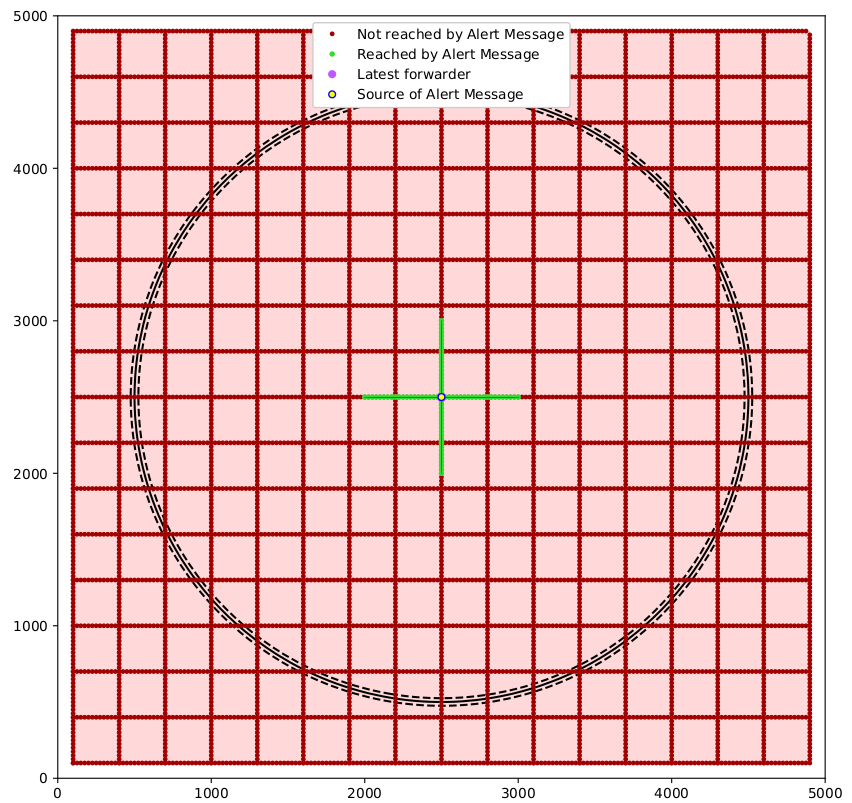
\includegraphics[width=0.8\textwidth]{immagini/grid-300/b1/fb-1hop}
			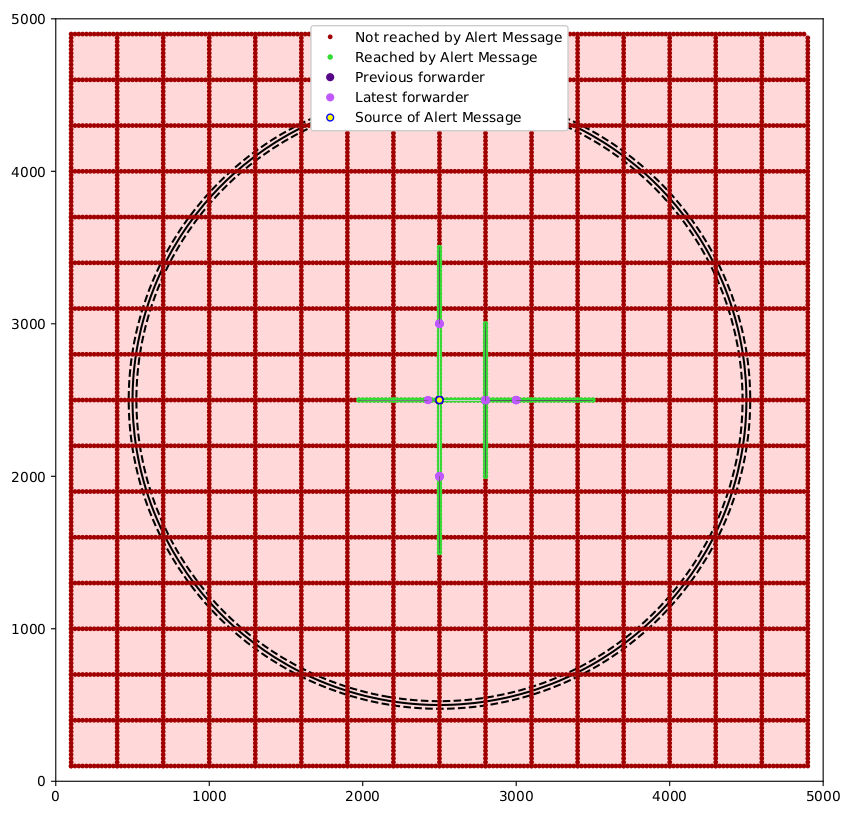
\includegraphics[width=0.8\textwidth]{immagini/grid-300/b1/fb-2hop}
			\caption{Fast-Broadcast after 1 hop (top) and 2 hops (bottom) in Grid scenario with 500 meters transmission range and with the Obstacle model}
			\label{fig:fb-b1-grid-transmission} 
		\end{figure}
	
		\begin{figure}[H]
			\centering
			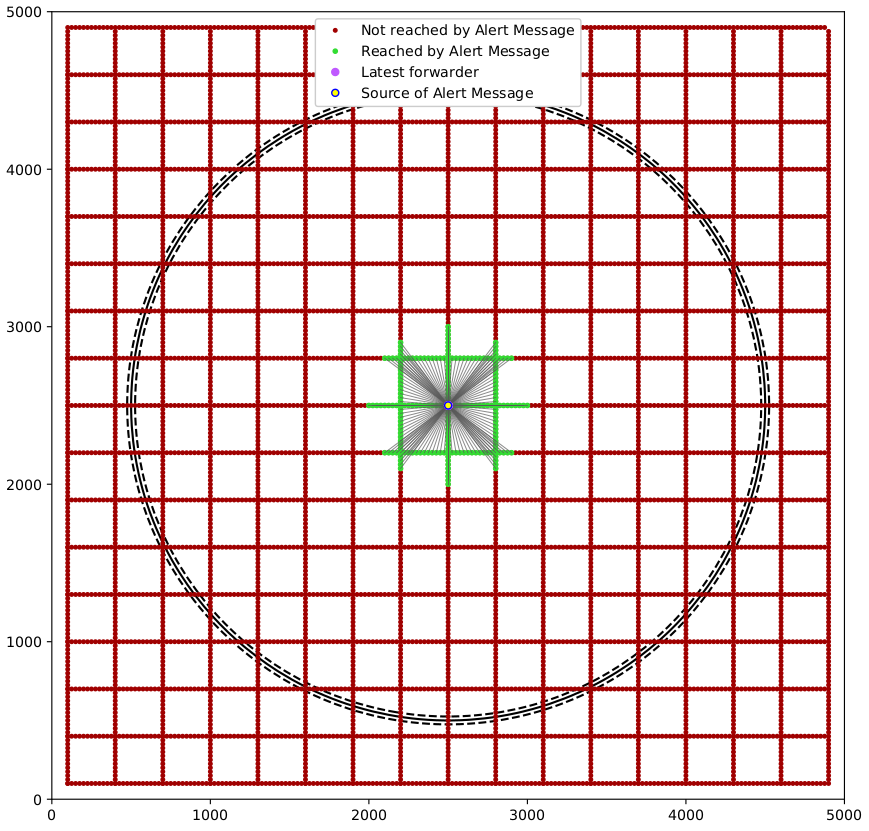
\includegraphics[width=0.8\textwidth]{immagini/grid-300/b0/roff-1hop}
			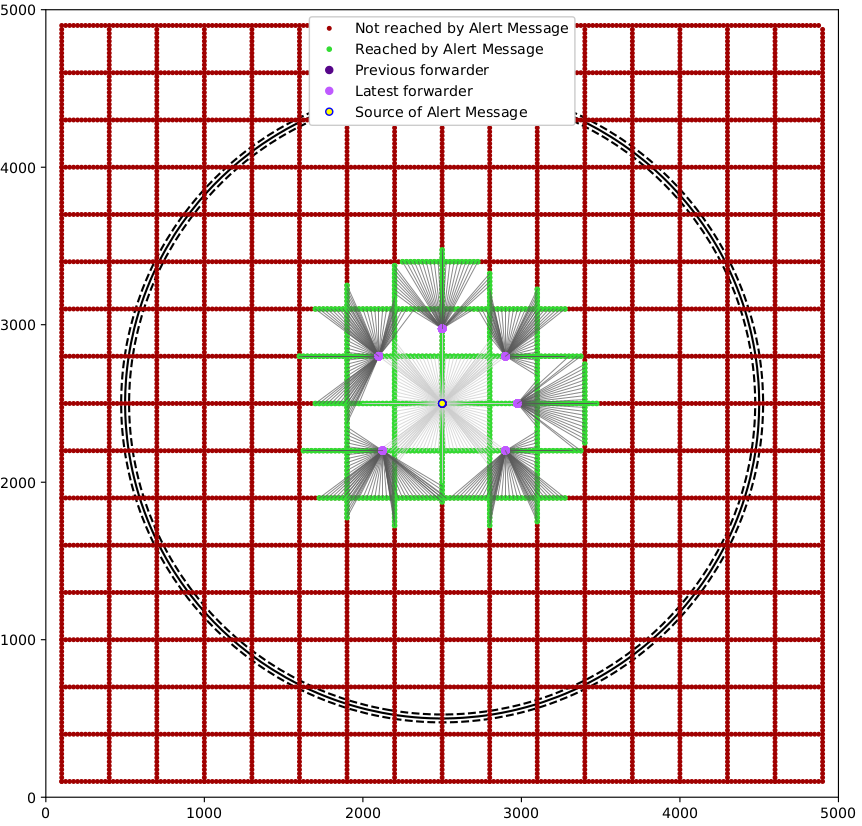
\includegraphics[width=0.8\textwidth]{immagini/grid-300/b0/roff-2hop}
			\caption{ROFF after 1 hop (top) and 2 hops (bottom) in Grid scenario with 500 meters transmission range and without the Obstacle model}
			\label{fig:roff-b0-grid-transmission}
		\end{figure}
	
		\begin{figure}[H]
			\centering
			\includegraphics[width=0.8\textwidth]{immagini/grid-300/b1/roff-1hop}
			\includegraphics[width=0.8\textwidth]{immagini/grid-300/b1/roff-2hop}
			\caption{ROFF after 1 hop (top) and 2 hops (bottom) in Grid scenario with 500 meters transmission range and with the Obstacle model}
			\label{fig:roff-b1-grid-transmission}
		\end{figure}
		
		If we focus on the Number Of Hops (Figure \ref{fig:grid-noh}), we notice that the introduction of buildings causes the number of hops to increases for transmission ranges of 100 and 500 meters, while decreases for 300 meters tranmission range. This is probably due to the fact that the distance between roads is also 300 meters and the starting vehicle is inside a junction. This means that the effect of buildings causes the signal to travel along roads, hopping from junction to junction, and reaching the circumference much faster. Another unusual observervation consists in ROFF with 100 meters transmission range, where the value increases by a lot. This case needs further examination in order to be explained. Apart from this case, ROFF achieves better results than Fast-Broadcast, with results 9\% and 3.47\% better for 300 and 500 meters transmission range respectively. 
		
		
		The analysis of the Number Of Slots (Figure \ref{fig:grid-nos}) shows similar results: the shadowing model causes the metric's value to rise in all configurations except for ROFF with 300 meters transmission range. ROFF continues to outperform Fast-Broadcast with results similar to those observed in the Platoon scenario. 
		
		
		Considering the Forwarding Node Number (Figure \ref{fig:grid-fnn}), the situation is much different than the previous scenario. It is possible to see in both graphs that ROFF's values are higher than Fast-Broadcast's across all configurations. Despite the almost-perfect suppression of redundant transmission works in a 1D scenario, as observed in the previous section, the mechanism does not seem to have much of an effect in a 2D scenario, regardless of the presence of buildings. A possible explanation of this phenomenon might be the one reported in Figure \ref{fig:2d-roff}, which indicates a possible Alert Message propagation process. Suppose that S is the previous forwarder: the other nodes on the circumference (distant txRange from S) are the elected FFCs which win the contention and relay the message. Due to how ROFF works, those nodes send the message at exactly the same time, hence if we focus on A and B we have a guaranteed collision area (the red area in Figure \ref{fig:2d-roff}). The nodes inside that collision area receive the forwarding from A and B at the same time and a collision occurs. As a consequence, they are not aware that the message has already been forwarded and some of them will fire their transmission. This process is repeated for every forward (and also for other FFCs other than A and B in the example) and so this could cause the increase in the FNN value. In other words, ROFF is guaranteed to cause the collision area shown in the example due to the exact waiting time calculation for nodes at the same distance from S. Fast-Broadcast is less affected by this problem since the waiting time calculation is not deterministic (the waiting time is chosen randomly from the interval [1...CW] where CW is calculated using Formula \ref{eq:contention-window}).
	
		\begin{figure}[H]
			\centering
			\includegraphics[width=0.5\textwidth]{immagini/2d-roff}
			\caption{Collision area in 2D scenarios for ROFF}
			\label{fig:2d-roff}
		\end{figure}

	\section{Los Angeles urban scenario}
		\label{sec:la-scenario}
		The next step consisted in expanding the 2D scenario with realistic urban data taken from OpenStreetMap and processed by SUMO as explained in Section \ref{sec:sumo}. In addition to the shadowing model, in this scenario (and also in the urban scenario regarding Padua, which will be presented in the next section), a \textit{smart junction} variant of the algorithms has been introduced in order to try to increase delivery ratios. 
		
		Figure \ref{fig:la-scenario} depicts the scenario with vehicles (green dots), buildings (pink polygons) and junctions (yellow polygons).
		
		
		All configurations are reported in Figure \ref{fig:la-overview}. In order to facilitate the understanding of the various configurations, the following graphs will utilize shades of color similar to those reported in Figure \ref{fig:la-overview} (e.g. graphs with shades of blue will represent a scenario without buildings and without junctions, while shades of orange will represent a scenario with buildings and with junctions). Parameters for this scenario are included in Table \ref{tab:la-25}.  
		
		\begin{figure}[H]
			\centering
			\includegraphics[width=0.90\textwidth]{immagini/la-25/la-scenario}
			\caption{Los Angeles urban scenario depiction}
			\label{fig:la-scenario}
		\end{figure}
		
		\begin{figure}[H]
			\centering
			\includegraphics[width=1.0\textwidth]{immagini/la-25/overview}
			\caption{Los Angeles urban scenario test overview}
			\label{fig:la-overview}
		\end{figure}
	
		\begin{table}[H]
			\def\arraystretch{1.1}
			\rowcolors{2}{D}{P}	
			\begin{tabularx}{\textwidth}{l | l  l}
				\rowcolor{I} {\large \textcolor{white}{Parameter}} & {\large \textcolor{white}{Value}} & {\large \textcolor{white}{}} \TBstrut  \\
				\toprule
				\endhead
				%			\midrule[1pt]
				\rowcolor{P} \multicolumn{3}{c}{Scenario configuration} \\
				\midrule[1pt]
				Latitude N								& 33.9654				& \textdegree		\\
				Latitude S								& 33.9478				& \textdegree		\\
				Longitude W								& -118.3260				& \textdegree		\\
				Longitude E								& -118.3055				& \textdegree		\\
				Road length 							& 1200	 				& m		\\
				Distance between vehicles 				& 25					& m		\\
				Circumference radius					& 1000					& m		\\
				Number of vehicles						& 1465					& 		\\
				Source of alert message position		& Center				&		\\
				Number of buildings						& 8241					&		\\
				Number of junctions						& 1288					&		\\	
				\midrule[1pt]
				\rowcolor{P} \multicolumn{3}{c}{Simulator configuration} \\
				\midrule[1pt]
				Shadowing model							& Obstacle Shadowing 	&		\\
				Junction modeling						& Yes					&		\\
				\midrule[1pt]
				Number of simulations per configuration	& 4500					&		\\
				\bottomrule
			\end{tabularx}
			\caption{Los Angeles urban scenario configuration}
			\label{tab:la-25}
		\end{table}
	
		\begin{figure}[H]
			\centering
			\includegraphics[width=1.0\textwidth]{immagini/la-25/b0/j0/tdr}
			\includegraphics[width=1.0\textwidth]{immagini/la-25/b0/j1/tdr}
			\includegraphics[width=1.0\textwidth]{immagini/la-25/b1/j0/tdr}
			\includegraphics[width=1.0\textwidth]{immagini/la-25/b1/j1/tdr}
			\caption{\textit{TDR} for Los Angeles urban scenario}
			\label{fig:la-25-tdr}
		\end{figure}
	
		\begin{figure}[H]
			\centering
			\includegraphics[width=1.0\textwidth]{immagini/la-25/b0/j0/tdroc}
			\includegraphics[width=1.0\textwidth]{immagini/la-25/b0/j1/tdroc}
			\includegraphics[width=1.0\textwidth]{immagini/la-25/b1/j0/tdroc}
			\includegraphics[width=1.0\textwidth]{immagini/la-25/b1/j1/tdroc}
			\caption{\textit{TDROC} for Los Angeles urban scenario}
			\label{fig:la-25-tdroc}
		\end{figure}

		\begin{figure}[H]
			\centering
			\includegraphics[width=1.0\textwidth]{immagini/la-25/b0/j0/noh}
			\includegraphics[width=1.0\textwidth]{immagini/la-25/b0/j1/noh}
			\includegraphics[width=1.0\textwidth]{immagini/la-25/b1/j0/noh}
			\includegraphics[width=1.0\textwidth]{immagini/la-25/b1/j1/noh}
			\caption{\textit{NOH} for Los Angeles urban scenario}
			\label{fig:la-25-noh}
		\end{figure}

		\begin{figure}[H]
			\centering
			\includegraphics[width=1.0\textwidth]{immagini/la-25/b0/j0/nos}
			\includegraphics[width=1.0\textwidth]{immagini/la-25/b0/j1/nos}
			\includegraphics[width=1.0\textwidth]{immagini/la-25/b1/j0/nos}
			\includegraphics[width=1.0\textwidth]{immagini/la-25/b1/j1/nos}
			\caption{\textit{NOS} for Los Angeles urban scenario}
			\label{fig:la-25-nos}
		\end{figure}

		\begin{figure}[H]
			\centering
			\includegraphics[width=1.0\textwidth]{immagini/la-25/b0/j0/fnn}
			\includegraphics[width=1.0\textwidth]{immagini/la-25/b0/j1/fnn}
			\includegraphics[width=1.0\textwidth]{immagini/la-25/b1/j0/fnn}
			\includegraphics[width=1.0\textwidth]{immagini/la-25/b1/j1/fnn}
			\caption{\textit{FNN} for Los Angeles urban scenario}
			\label{fig:la-25-fnn}
		\end{figure}
	
		It is possible to observe the effects of the Obstacle Shadowing model on \textit{Total Delivery Ratio} and \textit{Total Delivery Ratio On Circumference}. The effects are pretty mild across all configurations, but are more noticeable with lower transmission ranges (100 and 300 meters). For example, introducing the shadowing model without considering junctions leads to a decrease of 5.97\% (98.38 to 92.5) in \textit{TDR} (Figure \ref{fig:la-25-tdr}) with a transmission range of 100 meters and a decrease of 5\% (99.96 to 94.96) with transmission range of 300 meters for Fast-Broadcast. Results for ROFF are comparable, with decreases of 6.28\% and 5.73\% respectively.
		
		
		The decrease in \textit{TDROC} (Figure \ref{fig:la-25-tdr}) is much more noticeable, especially for the 100 meters transmission range. The value decrease by 16.11\% for Fast-Broadcast and 16.74\% for ROFF. This means that introducing building shadowing leads to more problems when the Alert Message has to reach farther distances. This phenomenon can be seen in Figure \ref{fig:la-coverage-fb100}.
		Vehicles not reached by the Alert Message are more concentrated towards the circumference instead of the center.
		
		\begin{figure}[H]
			\centering
			\includegraphics[width=1.0\textwidth]{immagini/la-25/la-coverage-fb100}
			\caption{Alert Message delivery for Los Angeles scenario with buildings and without junctions (Fast-Broadcast with 100 meters transmission range)}
			\label{fig:la-coverage-fb100}
		\end{figure}
		
		The introduction of the smart junction variants of the algorithms proves to be fairly effective, increasing \textit{TDR} by 3,52\% and 5,03\% when employing SJ-Fast-Broadcast instead of Fast-Broadcast for the scenario with buildings and transmission range of 100 and 300 meters respectively. Increases of the same magnitude can be noticed when utilizing SJ-ROFF instead of ROFF. With regards to \textit{TDROC}, both SJ-Fast-Broadcast and SJ-ROFF reach 100\% for 300 and 500 meters transmission ranges, while having a mild increase of around 3,40\% for 100 meters transmission range.
		
		
		Considering the Number Of Hops to reach the circumference (\ref{fig:la-25-noh}), we can observe that the introduction of the shadowing model leads to an increase in the metric's value across all algorithms. Comparing the first and third configuration, \textit{NOH} rises by 8.98\%, 53.74\% and 115.68\% for Fast-Broadcast, and by 3.85\%, 36.27\% and 64.69\% for ROFF, for the three increasing transmission ranges. We notice that:
		\begin{enumerate}
			\item the rise increases with the increase in transmission range;
			\item Fast-Broadcast is affected in a greater way by the shadowing model compared to ROFF.
		\end{enumerate}
		The first point is expected, since the one-hop progress is greater in a scenario with a higher transmission range. This leads to a greater probability for the signal to run into a building. In a scenario with a lower transmission range, transmissions have a lower probability to run into a building and follow more closely the road segment even without the effects of buildings. Hence, they are less likely to be influenced by the model. The second point may be due to the fact ROFF's Neighbor Table mechanism continues to work well to identify the FFC along the road segment, leading to a smaller increase in the number of hops.
		
		
		SJ-Fast-Broadcast and SJ-ROFF need less hops in order to reach the circumference than their counterparts which do not take junctions into consideration. This holds true for both scenarios with and without buildings. This is probably due to the additional transmissions inside junctions, which help to propagate the signal along road segments in a linear way, hence covering more space with each hop. SJ-ROFF performs better than SJ-Fast-Broadcast with regards to \textit{NOH}. The difference between the two algorithms decreases as the transmission range increases.
		
		
		Regarding \textit{NOS} (Figure \ref{fig:la-25-nos}), Fast-Broadcast results increase by 106.09\%, 1220\% and 3014\% while ROFF's ones increase by 111.11\% and 520\% for 300 and 500 meters transmission range, and decrease by 4.44\% for 100 meters transmission range, when going from a building-less scenario to a scenario with buildings. Moreover, Fast-Broadcast's values are 4412.82\%, 1636.84\% and 603.23\% higher than ROFF's values in the scenario with buildings. This goes to show the effect of empty space distribution on waiting times (here represented by the number of slots waited): when the distance between the FFC and the previous forwarder is close to the estimated transmission range, then Fast-Broadcast's waiting slots are pretty close to the minimum. But when obstacles are introduced, there might not be any PFC whose distance is close to the estimated transmission range. Hence, the FFC will wait a very long time. ROFF is not affected by this phenomenon thanks to the forwarding priority acquisition, as introduced in Chapter \ref{chapter:roff}. Comparing the third and fourth image in Figure \ref{fig:la-25-nos}, we can see that the introduction of junctions is beneficial for both algorithms, leading to a decrease in \textit{NOS}. This is a consequence of the abovementioned decrease in Number Of Hops.
			
		Concerning the Forwarding Node Number (Figure \ref{fig:la-25-fnn}), the value increases when the shadowing model is introduced. ROFF with 100 meters transmission range is the only configuration where the values decreases. This configuration needs further testing in order to be explained.
		The introduction of junctions brings about an increase in the number of forwardings for all algorithms, as expected. Focusing on the fourth image of Figure \ref{fig:la-25-fnn}, SJ-ROFF is affected greatly by this increase, almost equalling SJ-Fast-Broadcast with 100 meters transmission range, and with much greater \textit{FNN} values in 300 and 500 meters transmission range configurations. This might be caused by the introduction of transmissions inside junctions, which exacerbate the collision problem already reported in the previous section (Figure \ref{fig:2d-roff}), leading to an imperfect suppression of scheduled transmissions. The problem is not as severe as in the Grid scenario since the node distribution is less regular, but overall Fast-Broadcast performs better than ROFF in terms of \textit{FNN}.
	
	\section{Padua urban scenario}
		\label{sec:padua-urban}
		As reported in the previous section the Los Angeles scenario, despite being realistic, still had a certain degree of regularity for what concerns vehicle distribution and scenario topology. In fact, roads and sidewalks are pretty large and the overall road positioning resembles a Grid scenario. The next step in testing consisted in employing the algorithms in a more difficult scenario, with narrower roads and intersections, smaller (if any) sidewalks and pedestrian zones where no traffic is allowed. The chosen scenario is located in Padua and, as the previous one, data about the scenario have been retrieved by OSM and processed through SUMO. The scenario is depicted in Figure \ref{fig:padua-scenario}, while its configuration is reported in Table \ref{tab:padua-25}. 
		
		\begin{figure}[H]
			\centering
			\includegraphics[width=0.98\textwidth]{immagini/padua-25/padua-scenario}
			\caption{Padua urban scenario depiction}
			\label{fig:padua-scenario}
		\end{figure}
	
		\begin{table}[H]
			\def\arraystretch{1.1}
			\rowcolors{2}{D}{P}	
			\begin{tabularx}{\textwidth}{l | l  l}
				\rowcolor{I} {\large \textcolor{white}{Parameter}} & {\large \textcolor{white}{Value}} & {\large \textcolor{white}{}} \TBstrut  \\
				\toprule
				\endhead
				%			\midrule[1pt]
				\rowcolor{P} \multicolumn{3}{c}{Scenario configuration} \\
				\midrule[1pt]
				Latitude N								& 45.4171				& \textdegree		\\
				Latitude S								& 45.3981				& \textdegree		\\
				Longitude W								& 11.8654				& \textdegree		\\
				Longitude E								& 11.8923				& \textdegree		\\
				Road length 							& 1200	 				& m		\\
				Distance between vehicles 				& 25					& m		\\
				Circumference radius					& 1000					& m		\\
				Number of vehicles						& 1775					& 		\\
				Source of alert message position		& Center				&		\\
				Number of buildings						& 6322					&		\\
				Number of junctions						& 3231					&		\\	
				\midrule[1pt]
				\rowcolor{P} \multicolumn{3}{c}{Simulator configuration} \\
				\midrule[1pt]
				Shadowing model							& Obstacle Shadowing 	&		\\
				Junction modeling						& Yes					&		\\
				\midrule[1pt]
				Number of simulations per configuration	& 4500					&		\\
				\bottomrule
			\end{tabularx}
			\caption{Los Angeles urban scenario configuration}
			\label{tab:padua-25}
		\end{table}
	
		\begin{figure}[H]
			\centering
			\includegraphics[width=1.0\textwidth]{immagini/padua-25/b0/j0/tdr}
			\includegraphics[width=1.0\textwidth]{immagini/padua-25/b0/j1/tdr}
			\includegraphics[width=1.0\textwidth]{immagini/padua-25/b1/j0/tdr}
			\includegraphics[width=1.0\textwidth]{immagini/padua-25/b1/j1/tdr}
			\caption{\textit{TDR} for Padua urban scenario}
			\label{fig:padua-25-tdr}
		\end{figure}
		
		\begin{figure}[H]
			\centering
			\includegraphics[width=1.0\textwidth]{immagini/padua-25/b0/j0/tdroc}
			\includegraphics[width=1.0\textwidth]{immagini/padua-25/b0/j1/tdroc}
			\includegraphics[width=1.0\textwidth]{immagini/padua-25/b1/j0/tdroc}
			\includegraphics[width=1.0\textwidth]{immagini/padua-25/b1/j1/tdroc}
			\caption{\textit{TDROC} for Padua urban scenario}
			\label{fig:padua-25-tdroc}
		\end{figure}
		
		\begin{figure}[H]
			\centering
			\includegraphics[width=1.0\textwidth]{immagini/padua-25/b0/j0/noh}
			\includegraphics[width=1.0\textwidth]{immagini/padua-25/b0/j1/noh}
			\includegraphics[width=1.0\textwidth]{immagini/padua-25/b1/j0/noh}
			\includegraphics[width=1.0\textwidth]{immagini/padua-25/b1/j1/noh}
			\caption{\textit{NOH} for Padua urban scenario}
			\label{fig:padua-25-noh}
		\end{figure}
		
		\begin{figure}[H]
			\centering
			\includegraphics[width=1.0\textwidth]{immagini/padua-25/b0/j0/nos}
			\includegraphics[width=1.0\textwidth]{immagini/padua-25/b0/j1/nos}
			\includegraphics[width=1.0\textwidth]{immagini/padua-25/b1/j0/nos}
			\includegraphics[width=1.0\textwidth]{immagini/padua-25/b1/j1/nos}
			\caption{\textit{NOS} for Padua urban scenario}
			\label{fig:padua-25-nos}
		\end{figure}
		
		\begin{figure}[H]
			\centering
			\includegraphics[width=1.0\textwidth]{immagini/padua-25/b0/j0/fnn}
			\includegraphics[width=1.0\textwidth]{immagini/padua-25/b0/j1/fnn}
			\includegraphics[width=1.0\textwidth]{immagini/padua-25/b1/j0/fnn}
			\includegraphics[width=1.0\textwidth]{immagini/padua-25/b1/j1/fnn}
			\caption{\textit{FNN} for Padua urban scenario}
			\label{fig:padua-25-fnn}
		\end{figure}
	
		In this scenario the effects of obstacle shadowing on delivery ratios is quite large, especially for the 300 and 500 meters cases, for all algorithms. We have a decrease in \textit{TDR} (Figure \ref{fig:padua-25-tdr}) of around 65\% for Fast-Broadcast in both transmission ranges when introducing buildings (first and third images), which results in quite poor performances. The Smart Junction variants of Fast-Broadcast manages to reach pretty good results in Total Delivery Ratio (fourth image), with 72.1\% and 91.42\% for the two transmission ranges. ROFF's results are even worse before the introduction of junctions, with \textit{TDR} below 10\% for the lowest transmission range. Even in this case, SJ-ROFF manages to improve the values, slightly overcoming SJ-Fast-Broadcast's results.
		
		
		The same observations hold true even for \textit{TDROC} (\ref{fig:padua-25-tdr}). Hence, the benefits of junctions are twofold even for this scenario regarding delivery ratios.
		
		
		Concerning \textit{NOS}, the increase due to the obstacle model is even more pronounced than the previous scenario for both algorithms. Due to the lower coverage, it is possible that the few messages who reach the circumference go through a very irregular path and  one-hop progress is quite low. The introduction of junctions, as in the Los Angeles scenario, causes a decrease in \textit{NOH}. One anomalous results is ROFF with 100 meters transmission range, whose values shoots up by more than 232\% when comparing it with SJ-ROFF, and is much higher than SJ-Fast-Broadcast under the same conditions. This phenomenon might be due to the harsher vehicle distribution, obstacle and junction positioning which cause the signal to follow very long paths from the source to the circumference. With the other two transmission ranges, SJ-ROFF outperforms SJ-Fast-Broadcast.
		
		
		Results for \textit{NOH} and \textit{FNN} are comparable with the ones observed in previous scenarios.
		
		
	\section{Los Angeles smart city scenario}
		After the comparison of the algorithms in 2D scenarios, we wanted to test them in a mixed 2D-3D scenario, where drones were also employed. Drones are utilized in many military and civil applications, such as agriculture, environmental protection and traffic flow control. It is foreseeable that they will also be a part of the development of the so called \jquote{smart cities}, defined as \jquote{the use of discrete new technology applications such as RFID and Internet Of Things through more holistic conception of intelligent, integrated working that is closely linked to the concept of living and user generated services}\cite{smartCity}. One of the possible applications of drones in a urban scenario could make them help vehicles in Emergency Message Dissemination in order to exploit their greater field of view and bypass the effects of ground level shadowing and obstacles. 
		
		
		This scenario is built upon the Los Angeles urban scenario presented in Section \ref{sec:la-scenario}. Two layers of drones were added to the ground level of vehicles: 
		\begin{itemize}
			\item the first layer is situated at a height of 30 meters from ground level and employs 732 drones;
			\item the second layer, employing the same number of drones, is situated at a height of 60 meters.
		\end{itemize}
		Drones are more spaced from one another than vehicles, with an average distance of 50 meters. We also wanted to test the effects of the Obstacle Model on drones in this scenario. Since the maximum height of a building in the data retrieved from OpenStreetMap is 21.9 meters, drones would not have their line of sight affected by the obstacles. Hence, as an additional configuration of this scenario, all buildings have been heightened to be taller than the second layer of drones (e.g. every building is high 100 meters). 
		
		
		One important fact to notice is that, even if we have called the object placed inside the two layers \jquote{drones}, this scenario applies also if those objects were other kinds of network connected entities, such as customers' access points or IoT devices.
		
		Figure \ref{fig:la-smart-city} shows a representation of the two scenarios with buildings.
		
		\begin{figure}[H]
			\centering
			\includegraphics[width=0.95\textwidth]{immagini/la-smart-city-low}
			\includegraphics[width=0.95\textwidth]{immagini/la-smart-city-high}
			\caption{Los Angeles smart city scenario with real height buildings (top) and very high buildings (bottom)}
			\label{fig:la-smart-city}
		\end{figure}
		\newpage
		
		In this scenario, the \textit{TDR} metric considers delivery to all entities in the scenario (both vehicles and drones), while the circumference relative to the area of interest continues to be defined in the same way as the 2D Los Angeles urban scenario, hence TDROC concerns exclusively vehicles.
		
		
		All configurations are reported in Figure \ref{fig:la-smart-city-overview}, whose colors will guide the following graph results. Table \ref{tab:la-smart-city} reports all the scenario settings.
		
		\begin{figure}[H]
			\centering
			\includegraphics[width=0.7\textwidth]{immagini/la-smart-city/overview}
			\caption{Test overview of Los Angeles smart city scenario}
			\label{fig:la-smart-city-overview}
		\end{figure}
		
	\begin{table}[H]
		\def\arraystretch{1.1}
		\rowcolors{2}{D}{P}	
		\begin{tabularx}{\textwidth}{l | l  l}
			\rowcolor{I} {\large \textcolor{white}{Parameter}} & {\large \textcolor{white}{Value}} & {\large \textcolor{white}{}} \TBstrut  \\
			\toprule
			\endhead
			%			\midrule[1pt]
			\rowcolor{P} \multicolumn{3}{c}{Scenario configuration} \\
			\midrule[1pt]
			Circumference radius					& 1000					& m		\\
			Number of vehicles						& 1465					& 		\\
			Distance between vehicles 				& 25					& m		\\
			Source of alert message position		& Center				&		\\
			Number of drone layers					& 2						&		\\
			Height of first drone layer				& 30					& m		\\
			Number of drones in first layer			& 732					& 		\\
			Height of second drone layer			& 60					& m		\\
			Number of drones in second layer		& 732					& 		\\
			Distance between drones (average)		& 50					& m		\\
			Number of buildings						& 8241					&		\\
			Building heights						& Real, 100				& m		\\
			\midrule[1pt]
			\rowcolor{P} \multicolumn{3}{c}{Simulator configuration} \\
			\midrule[1pt]
			Shadowing model							& Obstacle Shadowing 	&		\\
			Junction modeling						& No					&		\\
			\midrule[1pt]
			Number of simulations per configuration	& 1000					&		\\
			\bottomrule
		\end{tabularx}
		\caption{Los Angeles urban scenario configuration}
		\label{tab:la-smart-city}
	\end{table}

	\begin{figure}[H]
		\centering
		\includegraphics[width=1.0\textwidth]{immagini/la-smart-city/b0/tdr}
		\includegraphics[width=1.0\textwidth]{immagini/la-smart-city/b1/h0/tdr}
		\includegraphics[width=1.0\textwidth]{immagini/la-smart-city/b1//h1/tdr}
		\caption{\textit{TDR} for Los angeles smart city scenario}
		\label{fig:la-smart-city-tdr}
	\end{figure}

	\begin{figure}[H]
		\centering
		\includegraphics[width=1.0\textwidth]{immagini/la-smart-city/b0/tdroc}
		\includegraphics[width=1.0\textwidth]{immagini/la-smart-city/b1/h0/tdroc}
		\includegraphics[width=1.0\textwidth]{immagini/la-smart-city/b1//h1/tdroc}
		\caption{\textit{TDROC} for Los angeles smart city scenario}
		\label{fig:la-smart-city-tdroc}
	\end{figure}
	
	\begin{figure}[H]
		\centering
		\includegraphics[width=1.0\textwidth]{immagini/la-smart-city/b0/noh}
		\includegraphics[width=1.0\textwidth]{immagini/la-smart-city/b1/h0/noh}
		\includegraphics[width=1.0\textwidth]{immagini/la-smart-city/b1//h1/noh}
		\caption{\textit{NOH} for Los angeles smart city scenario}
		\label{fig:la-smart-city-noh}
	\end{figure}

	\begin{figure}[H]
		\centering
		\includegraphics[width=1.0\textwidth]{immagini/la-smart-city/b0/nos}
		\includegraphics[width=1.0\textwidth]{immagini/la-smart-city/b1/h0/nos}
		\includegraphics[width=1.0\textwidth]{immagini/la-smart-city/b1//h1/nos}
		\caption{\textit{NOS} for Los angeles smart city scenario}
		\label{fig:la-smart-city-nos}
	\end{figure}

	\begin{figure}[H]
		\centering
		\includegraphics[width=1.0\textwidth]{immagini/la-smart-city/b0/fnn}
		\includegraphics[width=1.0\textwidth]{immagini/la-smart-city/b1/h0/fnn}
		\includegraphics[width=1.0\textwidth]{immagini/la-smart-city/b1//h1/fnn}
		\caption{\textit{FNN} for Los angeles smart city scenario}
		\label{fig:la-smart-city-fnn}
	\end{figure}

	Judging by the results shown in Figure \ref{fig:la-smart-city-tdr} and \ref{fig:la-smart-city-tdroc}, drones seem to help a lot in signal propagation thanks to their altitude. In fact, the scenario without buildings and with real-height buildings yield comparable results. In the third scenario, when the obstacles's heights exceed the second drone layer's height, the shadowing effect is more pronounced for lower transmission range configurations. Overall the total delivery ratio is still acceptable, with neither Fast-Broadcast or ROFF falling under 90\%. \textit{TDROC} in configurations with 100 meters transmission range is affected in a greater way. In fact, as specified above, in this scenario the \textit{TDROC} metric is only about vehicles on the ground, so the greater shadowing due to high buildings yields the expected results.
	
	
	The effects of obstacles on \textit{NOH} (Figure \ref{fig:la-smart-city-noh}) are consistent with those observed in previous scenarios. The metric's value further increases with high buildings, since the signal probably propagates more often on the ground instead of covering larger distances thanks to inter-street drone to vehicle communications. With high buildings the propagation is restrained inside the road, hence the effects of drones are much more limited.
	
	
	Concerning \textit{NOS} (Figure \ref{fig:la-smart-city-nos}), we can notice that the increase is much higher when going from obstacles with real heights to 100 meters high obstacles. For example, focusing on the 300 meters transmission range configuration, for Fast-Broadcast we have an increase of 64.71\% from the first to the second image and of 553.57\% from the second to the third. For ROFF those values are 27.27\% and 114.29\%. Once again, this phenomenon could be due to the same effect explained in the previous paragraph: with inter-street communication heavily impeded and the increase in \textit{NOH}, \textit{NOS} increases as a consequence.
	
	
	Focusing on the 300 and 500 meters transmission range configurations, \textit{FNN} (Figure \ref{fig:la-smart-city-fnn}) increases for Fast-Broadcast and ROFF, both when going from the first image to the second and from the second to the third. This is expected, since in both cases the shadowing effects are increased and a greater number of forwarders is necessary to cover the same area. For the 100 meters case, we can notice some anomalous results: Fast-Broadcast's value stays around the same number, while ROFF's decreases considerably in the last two scenarios. The same observation about collision areas in ROFF introduced in Section \ref{sec:grid} might explain this behaviour, but it would affect in a similar way also the 300 and 500 meters configurations. Hence, this phenomenon needs more thorough testing in order to be explained.
	
	
	Overall, the two main algorithms seem to work well even in this mixed 2D and 3D scenario, with similar advantages and disadvantages reported in previous urban scenarios.
	

	\section{Hello Message forging scenario}
		In all previous tests all entities participating in the message propagation told the truth about their position and did not try to manipulate the algorithms in order to hinder the delivery process. During our analysis we wanted to test how vulnerable the algorithms were to attacks where some malicious attacker tries to increase the end to end delay (the \textit{NOS} metric in our case). The attack consists in having a malicious node send fake Hello Messages bursts to vehicles during the Estimation Phase in order to mess with their estimations. These forged messages included fake information, mainly a wrong (overestimated) transmission range and fake IDs. We tested two different levels of severity on the attack: a low severity one, reported in Section \ref{sec:low-severity}, and a high severity one, reported in Section \ref{sec:high-severity}. Several percentages of affected vehicles (i.e. the vehicles which receive the forged Hello Message bursts) ranging from 0 to 50\% have been tested. Both tests were carried out using the Los Angeles urban scenario without the effect of the Obstacle Model. Only Fast-Broadcast and ROFF algorithms were tested.
		
		\subsection{Low severity attack} 
			In the low severity attack the effect of 150 different forged Hello Messages was tested. Each forged message reports a fake position such that the detected distances by the affected node (the receiver) ranges from 301 ($txRange + 1$) to 450 ($txRange + 150$). Parameters for this scenario are reported in Table \ref{tab:low-forging}.
			\label{sec:low-severity}
				\begin{table}[H]
				\def\arraystretch{1.1}
				\rowcolors{2}{D}{P}	
				\begin{tabularx}{\textwidth}{l | l  l}
					\rowcolor{I} {\large \textcolor{white}{Parameter}} & {\large \textcolor{white}{Value}} & {\large \textcolor{white}{}} \TBstrut  \\
					\toprule
					\endhead
					%			\midrule[1pt]
					\rowcolor{P} \multicolumn{3}{c}{Scenario configuration} \\
					\midrule[1pt]
					Vehicles affected by forging			& 0, 10, 20, 30, 40, 50 & \%	\\
					Number of forged messages				& 150					&		\\
					Forged distances						& 301, 302,...,450		&		\\
					\midrule[1pt]
					\rowcolor{P} \multicolumn{3}{c}{Simulator configuration} \\
					\midrule[1pt]
					Transmission power						& 4.6					& dBm	\\
					Transmission range						& 300					& m		\\
					Shadowing model							& No					&		\\
					Junction modeling						& No					&		\\
					\midrule[1pt]
					Number of simulations per configuration	& 1000					&		\\
					\bottomrule
				\end{tabularx}
				\caption{Low severity forging attack scenario configuration based on Los Angeles urban scenario}
				\label{tab:low-forging}
			\end{table}
			
			\begin{figure}[H]
				\centering
				\includegraphics[width=1.0\textwidth]{immagini/la-25/forging/nos-low-severity}
				\caption{\textit{NOS} for low severity forging scenario}
				\label{fig:low-forging}
			\end{figure}
					
			The hello forging attack fills the Neighbor Table of affected ROFF nodes with fake information about neighbors. The priority acquisition process is hence tainted by the fake PFCs, which get top priority due to forged distances being greater than the real transmission range. It is possible to see an increasing trend in ROFF results when the percentage of affected vehicles is increased. In fact, when more vehicles are affected by this attack, the probability of having affected nodes participating in the source-to-circumference message propagation increases, enlarging \textit{NOS} as a consequence.
			
			
			Fast-Broadcast is only affected in a small way when increasing the percentage of affected nodes from 0\% to 10\%. In fact, Fast-Broadcast utilizes only the estimated value of the transmission range for its waiting time computation, and does not take into account other information about the neighbors of a node. Hence, the only variable which affects Fast-Broadcast's \textit{NOS} is the maximum estimated transmission range, which is $450$ in this scenario . This value gets propagated throughout the network over time, despite the number of vehicles initially affected by the forging. As a consequence, the metric's value stabilizes after the percentage of affected vehicles is greater than 0\% and does not increase further when that percentage is increased.
			
			
			We can notice that ROFF's performances are similar to Fast-Broadcast's with 20\% of affected vehicles. After this threshold, ROFF's value increase further.
		
		\subsection{High severity attack}
			In the high severity attack the number of forged Hello Messages was increased to 1000. As a consequence, the fake positions included in the messages increased in a way such that the receivers detected distances ranging from 301 to 1300 meters. Parameters for this scenario are reported in Table \ref{tab:high-forging}.
			\label{sec:high-severity}
			\begin{table}[H]
				\def\arraystretch{1.1}
				\rowcolors{2}{D}{P}	
				\begin{tabularx}{\textwidth}{l | l  l}
					\rowcolor{I} {\large \textcolor{white}{Parameter}} & {\large \textcolor{white}{Value}} & {\large \textcolor{white}{}} \TBstrut  \\
					\toprule
					\endhead
					%			\midrule[1pt]
					\rowcolor{P} \multicolumn{3}{c}{Scenario configuration} \\
					\midrule[1pt]
					Vehicles affected by forging			& 0, 10, 20, 30, 40, 50 & \%	\\
					Number of forged messages				& 1000					&		\\
					Forged distances						& 301, 302,...,1300			&		\\
					\midrule[1pt]
					\rowcolor{P} \multicolumn{3}{c}{Simulator configuration} \\
					\midrule[1pt]
					Transmission power						& 4.6					& dBm	\\
					Transmission range						& 300					& m		\\
					Shadowing model							& No					&		\\
					Junction modeling						& No					&		\\
					\midrule[1pt]
					Number of simulations per configuration	& 1000					&		\\
					\bottomrule
				\end{tabularx}
				\caption{High severity forging attack scenario configuration based on Los Angeles urban scenario}
				\label{tab:high-forging}
			\end{table}
			
			\begin{figure}[H]
				\centering
				\includegraphics[width=1.0\textwidth]{immagini/la-25/forging/nos-high-severity}
				\caption{\textit{NOS} for high severity forging scenario}
				\label{fig:high-forging}
			\end{figure}
		
			In this case it is possible to observe that ROFF is affected a lot more than Fast-Broadcast by the attack. Even when jumping from 0\% to only 10\% of affected nodes, ROFF's \textit{NOS} increases more than tenfold, with a value 57.97\% higher than Fast-Broadcast under the same conditions. Fast-Broadcast is affected as well when going from 0\% to 10\%, but the increase is much lower. The reason is the same noticed in the previous Section: Fast-Broadcast is affected only by the maximum estimated transmission range (1300 meters in this scenario), while ROFF is also affected by the great number of information about fake neighbors. Higher percentages of affected vehicles increase the Number Of Slots even more for ROFF, while Fast-Broadcast caps out after 10\% and its metric's value does not increase.
			
			
			One can notice that making the attack stronger requires a smaller percentage of affected vehicles in order to make ROFF's the loser against Fast-Broadcast in this kind of confrontation. 
			
			
			As a consequence of these attacks, a possible solution could be the implementation of identification techniques between vehicles in order to discard forged messages.
	
	\section{Different vehicle density scenario}
		The previous scenarios all employed a distance between vehicles equal to 25 meters. Real vehicle distributions are obviously different than this idealistic scenario. Moreover, good broadcasting algorithms should work well regardless of vehicle distribution and density. Hence, in this section different vehicle distributions (generated by varying the distances between vehicles) have been tested. The scenario is based on the Padua urban scenario (Section \ref{sec:padua-urban}), with vehicle distances ranges from 5 to 45 meters, and without the effects of buildings. Obviously, a decrease in distance between vehicles implies an increase in vehicle density (and also on the total number of vehicles in the scenario). Parameters are reported in Table \ref{table:densities}.
		
		\begin{table}[H]
			\def\arraystretch{1.1}
			\rowcolors{2}{D}{P}	
			\begin{tabularx}{\textwidth}{l | l  l}
				\rowcolor{I} {\large \textcolor{white}{Parameter}} & {\large \textcolor{white}{Value}} & {\large \textcolor{white}{}} \TBstrut  \\
				\toprule
				\endhead
				\rowcolor{P} \multicolumn{3}{c}{Scenario configuration} \\
				\midrule[1pt]
				Distance between vehicles				& 5, 15, 25, 35, 45		& 		\\
				Number of vehicles						& 4975, 2856, 1776, 1318, 1072		& 		\\
				\midrule[1pt]
				\rowcolor{P} \multicolumn{3}{c}{Simulator configuration} \\
				\midrule[1pt]
				Transmission powers						& -7.0, 4.6, 13.4		& dBm	\\
				Transmission range						& 100, 300, 500			& m		\\
				Shadowing model							& No					&		\\
				Junction modeling						& No					&		\\
				\bottomrule
			\end{tabularx}
			\caption{Different vehicle densities scenario configuration based on Padua urban scenario}
			\label{table:densities}
		\end{table}
	
		\begin{figure}[H]
			\centering
			\includegraphics[width=0.8\textwidth]{immagini/density/fb/tdr}
			\includegraphics[width=0.8\textwidth]{immagini/density/roff/tdr}
			\caption{\textit{TDR} for Fast-Broadcast (top) and ROFF (bottom) with different distance between vehicles and transmission ranges}
			\label{fig:density-tdr}
		\end{figure}
	
		\begin{figure}[H]
			\centering
			\includegraphics[width=1.0\textwidth]{immagini/density/fb/tdroc}
			\includegraphics[width=1.0\textwidth]{immagini/density/roff/tdroc}
			\caption{\textit{TDROC} for Fast-Broadcast (top) and ROFF (bottom) with different distance between vehicles and transmission ranges}
			\label{fig:density-tdroc}
		\end{figure}
	
		\begin{figure}[H]
			\centering
			\includegraphics[width=1.0\textwidth]{immagini/density/fb/noh}
			\includegraphics[width=1.0\textwidth]{immagini/density/roff/noh}
			\caption{\textit{NOH} for Fast-Broadcast (top) and ROFF (bottom) with different distance between vehicles and transmission ranges}
			\label{fig:density-noh}
		\end{figure}
	
		\begin{figure}[H]
			\centering
			\includegraphics[width=0.9\textwidth]{immagini/density/fb/nos-1}
			\includegraphics[width=0.9\textwidth]{immagini/density/fb/nos-2}
			\includegraphics[width=0.9\textwidth]{immagini/density/roff/nos}
			\caption{\textit{NOS} for Fast-Broadcast (top) and ROFF (bottom) with different distance between vehicles and transmission ranges}
			\label{fig:density-nos}
		\end{figure}
	
		\begin{figure}[H]
			\centering
			\includegraphics[width=1.0\textwidth]{immagini/density/fb/fnn-1}
			\includegraphics[width=1.0\textwidth]{immagini/density/roff/fnn-1}
			\caption{\textit{FNN} for Fast-Broadcast (top) and ROFF (bottom) with different distance between vehicles and transmission ranges}
			\label{fig:density-fnn-1}
		\end{figure}
	
		\begin{figure}[H]
			\centering
			\includegraphics[width=1.0\textwidth]{immagini/density/fb/fnn-2}
			\includegraphics[width=1.0\textwidth]{immagini/density/roff/fnn-2}
			\caption{\textit{FNN} for Fast-Broadcast (top) and ROFF (bottom) with different distance between vehicles and transmission ranges (different angle)}
			\label{fig:density-fnn-2}
		\end{figure}
	
		Figure \ref{fig:density-tdr} and \ref{fig:density-tdr} show optimal delivery ratios both total and on the circumference. We can see a small drop in the metrics' values for the 100 meters transmission range and 5 meters vehicle distance configurations. This might be due to higher collisions near the forwarders, which cause the signal to propagate unevenly to all areas of the scenario. Despite this, the values are still acceptable for both algorithms.
		
		
		Concerning NOS (Figure \ref{fig:density-noh}), we notice that ROFF achieves better results in every case. For both algorithms, different vehicle densities do not seem to affect the number of hops by much. This means that the algorithms manage to designate a distant PFC as next forwarder in both high and low density scenarios, with ROFF designation working better as noticed in previous tests.
		
		
		Figure \ref{fig:density-nos} show that \textit{NOS} decreases as the transmission range decreases for Fast-Broadcast. This phenomenon is also due to the decrease in \textit{NOH} noticed in the previous paragraph. We notice how \textit{NOS} increases as the vehicle distance increases (hence the density decreases) under the 100 meters transmission range condition. This is expected, since the FFC can be quite far from the 100 meters mark which guarantees the minimum waiting time for each hop. Hence, the designated PFC could end up waiting a lot longer than a scenario with higher density.
		ROFF is not affected by either transmission range and vehicle distance due to its waiting time calculation.
		
		
		With 500 meters transmission range a positive correlation can be noticed for Fast-Broadcast's FNN (Figure \ref{fig:density-fnn-1} and \ref{fig:density-fnn-2}). In fact, the value increases as vehicle density increases. This can be explained by the greater number of node waiting the exact same waiting time after a forwarding, which results in a greater number of redundant transmissions. 
		For both algorithms, a dramatic increase in \textit{FNN} appears when decreasing the transmission range from 300 to 100 meters. With a reduced transmission range, every retransmission reaches a lower number of nodes.
		
	
	\section{Smaller contention window}
		\label{sec:smaller-cw}
		All previous tests involving Fast-Broadcast have been carried out with a contention window ranging from 32 to 1024 slots. This interval is so wide in order to guarantee correct waiting time calculation even in high vehicle density scenarios. Fast-Broadcast's results on Number Of Slots could benefit from using a narrower contention window. In this scenario, based on the Los Angeles urban scenario, a contention window ranging from 16 to 128 slots will be utilized. Parameters for this scenario are reported in Table \ref{table:fb-cw}.
		\begin{table}[H]
			\def\arraystretch{1.1}
			\rowcolors{2}{D}{P}	
			\begin{tabularx}{\textwidth}{l | l  l}
				\rowcolor{I} {\large \textcolor{white}{Parameter}} & {\large \textcolor{white}{Value}} & {\large \textcolor{white}{}} \TBstrut  \\
				\toprule
				\endhead
				\midrule[1pt]
				\rowcolor{P} \multicolumn{3}{c}{Simulator configuration} \\
				\midrule[1pt]
				Shadowing model							& No					&		\\
				Junction modeling						& No					&		\\
				\midrule[1pt]
				\rowcolor{P} \multicolumn{3}{c}{Protocols configuration} \\
				\midrule[1pt]
				%			Protocols tested						& \makecell{FB, ROFF, STATIC100, \\ STATIC300, STATIC500} & \\
				FB contention window					& [16, 128], [32, 1024]	& slot	\\
				ROFF distance range (\textit{k} parameter) & 1					&		\\	
				\midrule[1pt]
				Number of simulations per configuration	& 600					&		\\
				\bottomrule
			\end{tabularx}
			\caption{Contention window scenario configuraton based on Los Angeles urban scenario}
			\label{table:fb-cw}
		\end{table}
	
		\begin{figure}[H]
			\centering
			\includegraphics[width=1.0\textwidth]{immagini/la-25/cw/16/tdr}
			\includegraphics[width=1.0\textwidth]{immagini/la-25/cw/32/tdr}
			\caption{\textit{TDR} for [16, 128] contention window (top) and [32, 1024] contention window (bottom)}
			\label{fig:la-cw-tdr}
		\end{figure}
	
		\begin{figure}[H]
			\centering
			\includegraphics[width=1.0\textwidth]{immagini/la-25/cw/16/tdroc}
			\includegraphics[width=1.0\textwidth]{immagini/la-25/cw/32/tdroc}
			\caption{\textit{TDROC} for [16, 128] contention window (top) and [32, 1024] contention window (bottom)}
			\label{fig:la-cw-tdroc}
		\end{figure}
	
		\begin{figure}[H]
			\centering
			\includegraphics[width=1.0\textwidth]{immagini/la-25/cw/16/noh}
			\includegraphics[width=1.0\textwidth]{immagini/la-25/cw/32/noh}
			\caption{\textit{NOH} for [16, 128] contention window (top) and [32, 1024] contention window (bottom)}
			\label{fig:la-cw-noh}
		\end{figure}
	
		\begin{figure}[H]
			\centering
			\includegraphics[width=1.0\textwidth]{immagini/la-25/cw/16/nos}
			\includegraphics[width=1.0\textwidth]{immagini/la-25/cw/32/nos}
			\caption{\textit{NOS} for [16, 128] contention window (top) and [32, 1024] contention window (bottom)}
			\label{fig:la-cw-nos}
		\end{figure}
	
		\begin{figure}[H]
			\centering
			\includegraphics[width=1.0\textwidth]{immagini/la-25/cw/16/fnn}
			\includegraphics[width=1.0\textwidth]{immagini/la-25/cw/32/fnn}
			\caption{\textit{FNN} for [16, 128] contention window (top) and [32, 1024] contention window (bottom)}
			\label{fig:la-cw-fnn}
		\end{figure}
	
		Before starting to compare the metrics, we can notice that ROFF's results for both contention windows do not change: this is obvious, since the change in contention window affects only Fast-Broadcast (and its STATIC variants). Next, the same patterns between Fast-Broadcast and the STATIC protocols identified in previous tests regarding the underestimation, correct estimation and overestimation of transmission range continue to be true even for the lower contention window.
		
		
		The two different contention windows do not cause any significant difference in delivery ratios and \textit{NOH}. The smaller contention window brings about a big improvement in \textit{NOS}, especially for the 100 meters transmission range configuration, where the metric improves by 361.62\% for Fast-Broadcast. For the 300 meters transmission range, the metric improves by 56\%, coming close to ROFF's value, equal to 9 slots. However, this improvement comes with a cost: looking at FNN (Figure \ref{fig:la-cw-fnn}), we can see that Fast-Broadcast's metric worsens by 97.05\% and 254.29\% for the two highest transmission range. This means that the waiting time difference between PFCs is not long enough to guarantee suppression of redundant transmissions for the current vehicle density. Given a smaller contention window, more vehicles could end up waiting the exact same number of slots, hence resulting in multiple transmissions being fired simultaneously and needlessly. However, \textit{FNN} does not increase by much for the 100 meters transmission range, and the decrease in \textit{NOS} is the greatest: this means that for a lower number of PFCs (lower transmission range means lower number of neighbors for each node, hence a lower number of PFCs) the smaller contention window actually brings benefits all across the board. 
		
		
		These observation could suggest that a dynamic contention window, function of node density, number of neighbors or both could benefit Fast-Broadcast greatly.
		
	\section{Number of Hello Messages computation}
		All previous tests focused on metrics concerning the Broadcast Phase, i.e. the phase after the event whose information has to be delivered to a certain area has already happened. We deemed also important the analysis of the Estimation Phase, i.e. the phase where nodes exchange information about their position, speed and other data in order to get to know their neighbors. In fact, both Fast-Broadcast and ROFF need nodes to exchange some Hello Message with each other in order to make the Alert Message delivery efficient. The focus of this analysis will mainly regard the number of Hello Messages sent, and will show how the number of Hello Messages required by Fast-Broadcast is a lot lower than those required by ROFF. 
		
		The following analysis is based on the theoretical formulation of the algorithms and on a simplified version of the Grid scenario (Section \ref{sec:grid}), with 100, 300 and 500 meters transmission range (\textit{txRange}), as usual.  For Fast-Broadcast, whose analysis has proven to be more diffcult, we are interested in a rough estimation of the number of Hello Messages instead of the exact number. 
		
		Suppose we have a 1200x1200 meters grid with 5 north-south and 5 east-west roads, where vehicles are placed every 25 meters. In total, the scenario is composed of 455 vehicles. Since both algorithms utilizes \textit{turns} (or \textit{Beacon Intervals}, as they are called in ROFF), i.e. vehicles wait on average a certain amount of time in between Hello Message transmissions, the comparison between the number of Hello Message sent can be carried out by comparing the number of messages sent for each turn/Beacon Interval. For ROFF, the calculation is pretty simple: each vehicle sends a Hello Message every turn. As a consequence, in the scenario at hand, ROFF sends 455 Hello Messages for each turn. For Fast-Broadcast, the estimation depends on how transmission ranges intersect with each other. The maximum number of Hello Messages sent each turn is bounded from above by the number of circumferences with radius \textit{txRange} such that the intersection between the circumferences' area is maximum and the center of each circumference do not lie inside another circumference. Based on this observation, a rough estimation of the number of Hello Message can be seen in Figure \ref{fig:hello-fb}, where the purple dots represent vehicles sending Hello Messages.
		
		\begin{figure}[H]
			\centering
			\includegraphics[width=0.4\textwidth]{immagini/hello-100}
			\includegraphics[width=0.4\textwidth]{immagini/hello-300}
			\includegraphics[width=0.4\textwidth]{immagini/hello-500}
			\caption{Number of Hello Messages sent for Fast-Broadcast with 100 (top), 300 (middle) and 500 (bottom) meters transmission range}
			\label{fig:hello-fb}
		\end{figure}
		
		By enumeration it is possible to count the number of nodes which send the Alert Message. Table \ref{tab:hello-messages} shows the number of Hello Messages sent for every turn for different transmission ranges. As we can see, ROFF transmits a constant number of messages for every turn and that number does not decrease with transmission range increase. Instead, Fast-Broadcast transmits a much lower number of messages, with values decreasing with greater transmission ranges. The huge number of Hello Messages sent by ROFF could cause problems such as greater overhead and more collisions.
		
		
		In any case, further experimental tests are required to confirm the outcomes of this qualitative analysis.
		
		\begin{table}[H]
			\def\arraystretch{1.2}
			\centering
			\begin{tabular}{|p{4cm}|p{2cm}|p{2cm}|p{2cm}|ll} 
				\cline{1-4}
				\textbf{Protocol} & \multicolumn{3}{c|}{\textbf{Number of Hello Messages}}  &   \\ 
				\cline{2-4}
				& \textit{100m} & \textit{300m} & \textit{500m} &  &   \\ 
				\cline{1-4}
				Fast-Broadcast          & 89          & 20          & 9          &  &   \\ 
				\cline{1-4}
				ROFF          & \multicolumn{3}{c|}{455}          &  &   \\
				\cline{1-4}
			\end{tabular}
			\caption{Number of Hello Messages sent for every turn}
			\label{tab:hello-messages}
		\end{table}
	         
% !TEX encoding = UTF-8
% !TEX TS-program = pdflatex
% !TEX root = ../tesi.tex


\chapter{Conclusions}
		\label{sec:comparison}
	After thorough testing in several scenarios of increasing complexity, Fast-Broadcast, ROFF and their Smart Junction variants have been compared. While the original algorithms lacked in delivery ratios, especially in more complicated scenarios, such as Padua, where the shadowing effects of the Obstacle Model were more pronounced, the SJ variants managed to reach good and comparable levels of coverage across all the network at the cost of increasing the number of forwarding nodes. Given the similar increase in metrics for both algorithms when junctions are introduced, the final comparison will focus on the original ROFF and Fast-Broadcast algorithms. As is often the case in these kind of analysis, no algorithm emerges as clear winner across the board. Instead, each scheme has its own pros and cons, which will be analyzed in the following paragraphs.
	
	
	The comparison between the number of Hello Messages sent makes Fast-Broadcast a clear winner, with a decreasing number of messages sent when transmission range increases. Instead, ROFF requires every vehicle to transmit its own Hello Message during the estimation phase in order to reach good performances. A good knowledge of the neighborhood is hence paramount for ROFF. Fast-Broadcast can work with a lower number of transmitted messages since the only information needed is the maximum estimated transmission range. 
	
	
	After this consideration about the Estimation Phase, the comparison can now consider the Broadcast Phase after the initial sending of the Alert Message. Several metrics have been utilized in order to test the effectiveness of the algorithms under different points of view. As already explained earlier, both schemes manage to score comparable results from the delivery ratios point of view. The real advantage of ROFF concerns the number of hops and slots to reach the area of interest. ROFF achieves much better results than Fast-Broadcast especially for lower transmission ranges. With higher transmission ranges, the gap is much narrower. The reason that causes ROFF's higher performances is the much more reliable farthest forwarder candidate selection, which reduces hops, and the lower waiting time due to a more precise scheduling and waiting time computation, which reduces the number of slots. This comes with a cost: the number of nodes who forward the Alert Message is higher for ROFF compared to Fast-Broadcast for the majority of 2D and 3D scenarios. One possible cause which concerns collision areas due to a "too perfect" schedulation has been theorised in Section \ref{sec:grid}. A greater number of forwarders could contribute to a dissemination-hindering congestion across the network, especially when paired with other bandwidth consuming applications, which is obviously an undesirable property for a multi-hop broadcasting protocol.
	
	
	Another point against ROFF is its vulnerability to Hello Message forging, which causes the number of slots waited to increase when the percentage of affected vehicles increases. After a certain threshold, which depends on the severity of the attack, ROFF performs worse than Fast-Broadcast in terms of waited slots.
	
	
%		Alert MEssage overhead %todo  
	
	
	Table \ref{table:pros-cons} summarises all the algorithms' pros and cons.
	
	\begin{table}[H]
		\def\arraystretch{1.2}
%			\rowcolors{2}{D}{P}	
		\begin{tabularx}{\textwidth}{|l | R{2cm} | c | p{2cm} | l | }
%				\rowcolor{I} {\large \textcolor{white}{Parameter}} & {\large \textcolor{white}{Value}} & {\large \textcolor{white}{}} \TBstrut  \\
			\cline{1-5}
			\multicolumn{2}{|r|}{\textbf{Fast-Broadcast}} & \textbf{Feature} & \multicolumn{2}{|l|}{\textbf{ROFF}} \\
			\endhead
			\cline{1-5}
			\yellowcheck & Medium & Number of slots & Low & \greencheck \\ 
			\yellowcheck & Medium & Number of hops & Low & \greencheck \\  
			\greencheck  & Low & Number of Hello Messages & High & \redx \\ 
			\yellowcheck & Medium & Number of forwarding nodes & High & \redx \\   
			\greencheck  & Low & Vulnerability to forging & High & \redx \\
			\cline{1-5}
		\end{tabularx}
		\caption{Fast-Broadcast and ROFF's pros and cons}
		\label{table:pros-cons}
	\end{table}
	
	
	Considering all the abovementioned advantages and disadvantages of the two algorithms, and considering also the necessity of quick propagation which characterises alert situations, the algorithm which seems to offer more advantages is ROFF. The low number of hops and slots helps reducing the end-to-end delay, delivering the information quickly to the area of interest.  
		
	\section{Future works}
		\label{sec:future}
		The simulations carried out in Section \ref{sec:smaller-cw} showed how a smaller contention window could benefit Fast-Broadcast's performances on the number of slots waited. A possible extension of Fast-Broadcast which could increase its performances could employ a dynamic contention window based on vehicle density. 
		
		
		The smart junction extension to the algorithms in this work operates correctly under the assumption that vehicles know junctions' locations, for example via a GPS system. Even though these kind of information is widespread nowadays, having a working broadcasting protocol even in emergency situations where GPS system are not available would be desirable. Hence, one possible proposal could identify junctions based on how many directions a vehicle receives other Hello Messages from. For example, a vehicle \textit{f} receiving three different messages from three different directions such that the angle between \textit{f} and the senders is greater than {270\textdegree} could identify itself as a vehicle inside a junction. This backup mode could prove itself useful even when more accurate data about a location are not available or have not been updated in a long time (e.g., smaller cities, rural areas, etc.).
		
		
		Lastly, the current work employed only multi-hop broadcasting protocols in the comparison. An extension of this work could compare the achieved results with probabilist or single-hop protocols (Section \ref{sec:emd}) to test the effectiveness of other state of the art algorithms.
		
		
%
%confronti pro contro
%pro fb:
%
%-minor overhead nell'invio dell'alert message
           
%% !TEX encoding = UTF-8
% !TEX TS-program = pdflatex
% !TEX root = ../tesi.tex

%**************************************************************
\chapter{Analisi dei requisiti}
\label{cap:analisi-requisiti}
%**************************************************************

\intro{Breve introduzione al capitolo}\\

\section{Casi d'uso}

Per lo studio dei casi di utilizzo del prodotto sono stati creati dei diagrammi.
I diagrammi dei casi d'uso (in inglese \emph{Use Case Diagram}) sono diagrammi di tipo \gls{uml} dedicati alla descrizione delle funzioni o servizi offerti da un sistema, così come sono percepiti e utilizzati dagli attori che interagiscono col sistema stesso.
Essendo il progetto finalizzato alla creazione di un tool per l'automazione di un processo, le interazioni da parte dell'utilizzatore devono essere ovviamente ridotte allo stretto necessario. Per questo motivo i diagrammi d'uso risultano semplici e in numero ridotto.

\begin{figure}[!h] 
    \centering 
    \includegraphics[width=0.9\columnwidth]{usecase/scenario-principale} 
    \caption{Use Case - UC0: Scenario principale}
\end{figure}

\begin{usecase}{0}{Scenario principale}
\usecaseactors{Sviluppatore applicativi}
\usecasepre{Lo sviluppatore è entrato nel plug-in di simulazione all'interno dell'IDE}
\usecasedesc{La finestra di simulazione mette a disposizione i comandi per configurare, registrare o eseguire un test}
\usecasepost{Il sistema è pronto per permettere una nuova interazione}
\label{uc:scenario-principale}
\end{usecase}

\section{Tracciamento dei requisiti}

Da un'attenta analisi dei requisiti e degli use case effettuata sul progetto è stata stilata la tabella che traccia i requisiti in rapporto agli use case.\\
Sono stati individuati diversi tipi di requisiti e si è quindi fatto utilizzo di un codice identificativo per distinguerli.\\
Il codice dei requisiti è così strutturato R(F/Q/V)(N/D/O) dove:
\begin{enumerate}
	\item[R =] requisito
    \item[F =] funzionale
    \item[Q =] qualitativo
    \item[V =] di vincolo
    \item[N =] obbligatorio (necessario)
    \item[D =] desiderabile
    \item[Z =] opzionale
\end{enumerate}
Nelle tabelle \ref{tab:requisiti-funzionali}, \ref{tab:requisiti-qualitativi} e \ref{tab:requisiti-vincolo} sono riassunti i requisiti e il loro tracciamento con gli use case delineati in fase di analisi.

\newpage

\begin{table}%
\caption{Tabella del tracciamento dei requisti funzionali}
\label{tab:requisiti-funzionali}
\begin{tabularx}{\textwidth}{lXl}
\hline\hline
\textbf{Requisito} & \textbf{Descrizione} & \textbf{Use Case}\\
\hline
RFN-1     & L'interfaccia permette di configurare il tipo di sonde del test & UC1 \\
\hline
\end{tabularx}
\end{table}%

\begin{table}%
\caption{Tabella del tracciamento dei requisiti qualitativi}
\label{tab:requisiti-qualitativi}
\begin{tabularx}{\textwidth}{lXl}
\hline\hline
\textbf{Requisito} & \textbf{Descrizione} & \textbf{Use Case}\\
\hline
RQD-1    & Le prestazioni del simulatore hardware deve garantire la giusta esecuzione dei test e non la generazione di falsi negativi & - \\
\hline
\end{tabularx}
\end{table}%

\begin{table}%
\caption{Tabella del tracciamento dei requisiti di vincolo}
\label{tab:requisiti-vincolo}
\begin{tabularx}{\textwidth}{lXl}
\hline\hline
\textbf{Requisito} & \textbf{Descrizione} & \textbf{Use Case}\\
\hline
RVO-1    & La libreria per l'esecuzione dei test automatici deve essere riutilizzabile & - \\
\hline
\end{tabularx}
\end{table}%             % Concept Preview
%% !TEX encoding = UTF-8
% !TEX TS-program = pdflatex
% !TEX root = ../tesi.tex

%**************************************************************
\chapter{Progettazione e codifica}
\label{cap:progettazione-codifica}
%**************************************************************

\intro{Breve introduzione al capitolo}\\

%**************************************************************
\section{Tecnologie e strumenti}
\label{sec:tecnologie-strumenti}

Di seguito viene data una panoramica delle tecnologie e strumenti utilizzati.

\subsection*{Tecnologia 1}
Descrizione Tecnologia 1.

\subsection*{Tecnologia 2}
Descrizione Tecnologia 2

%**************************************************************
\section{Ciclo di vita del software}
\label{sec:ciclo-vita-software}

%**************************************************************
\section{Progettazione}
\label{sec:progettazione}

\subsubsection{Namespace 1} %**************************
Descrizione namespace 1.

\begin{namespacedesc}
    \classdesc{Classe 1}{Descrizione classe 1}
    \classdesc{Classe 2}{Descrizione classe 2}
\end{namespacedesc}


%**************************************************************
\section{Design Pattern utilizzati}

%**************************************************************
\section{Codifica}
             % Product Prototype
%% !TEX encoding = UTF-8
% !TEX TS-program = pdflatex
% !TEX root = ../tesi.tex

%**************************************************************
\chapter{Verifica e validazione}
\label{cap:verifica-validazione}
%**************************************************************             % Product Design Freeze e SOP
%% !TEX encoding = UTF-8
% !TEX TS-program = pdflatex
% !TEX root = ../tesi.tex

%**************************************************************
\chapter{Conclusioni}
\label{cap:conclusioni}
%**************************************************************

%**************************************************************
\section{Consuntivo finale}

%**************************************************************
\section{Raggiungimento degli obiettivi}

%**************************************************************
\section{Conoscenze acquisite}

%**************************************************************
\section{Valutazione personale}
             % Conclusioni
%\appendix                               
%% !TEX encoding = UTF-8
% !TEX TS-program = pdflatex
% !TEX root = ../tesi.tex

%**************************************************************
\chapter{Appendice A}
%**************************************************************

\epigraph{Citazione}{Autore della citazione}



             % Appendice A
\appendix
% !TEX encoding = UTF-8
% !TEX TS-program = pdflatex
% !TEX root = ../tesi.tex

\chapter{Fast-Broadcast modifications}
	\label{chapter:fbmod}
	The previous work \cite{ROM2017} utilized a version of Fast-Broadcast in which vehicles having origin-vehicle distance smaller than origin-sender distance suppressed their scheduled transmission since they do not contribute in the outward propagation of the message. In the following graphs, the old version will be called \textit{TD-Fast-Broadcast} (as in \textit{Triangular-Distance-Fast-Broadcast}). The aim of this appendix is to show the reasons why this additional check has been removed in the version of the Fast-Broadcast algorithm used in this work thanks to simulations which employed two scenarios. More in detail, the aim of these simulations has been twofold:
	\begin{itemize}
		\item show that TD-Fast-Broadcast performs worse than Fast-Broadcast in terms of delivery ratios in difficult scenarios with buildings, particularly the Padua urban scenario;
		\item show that Fast-Broadcast is non-pejorative in all metrics in scenarios where TD-Fast-Broadcast did not show delivery ratio problems, such as the Los Angeles urban scenario.
	\end{itemize}

	\section{Fast-Broadcast's improvement on delivery ratios}
		\begin{figure}[H]
			\centering
			\includegraphics[width=1.0\textwidth]{immagini/td-fb-pd/td-fb/tdr}
			\includegraphics[width=1.0\textwidth]{immagini/td-fb-pd/fb/tdr}
			\caption{\textit{TDR} for TD-Fast-Broadcast (top) and Fast-Broadcast (bottom) for Padua urban scenario}
			\label{fig:td-tdr}
		\end{figure}
	
		\begin{figure}[H]
			\centering
			\includegraphics[width=1.0\textwidth]{immagini/td-fb-pd/td-fb/tdroc}	
			\includegraphics[width=1.0\textwidth]{immagini/td-fb-pd/fb/tdroc}
			\caption{\textit{TDROC} for TD-Fast-Broadcast (top) and Fast-Broadcast (bottom) for Padua urban scenario}
			\label{fig:td-tdroc}
		\end{figure}
	
		\begin{figure}[H]
			\centering
			\includegraphics[width=1.0\textwidth]{immagini/td-fb-pd/td-fb/noh}	
			\includegraphics[width=1.0\textwidth]{immagini/td-fb-pd/fb/noh}
			\caption{\textit{NOH} for TD-Fast-Broadcast (top) and Fast-Broadcast (bottom) for Padua urban scenario}
			\label{fig:td-noh}
		\end{figure}
	
		\begin{figure}[H]
			\centering
			\includegraphics[width=1.0\textwidth]{immagini/td-fb-pd/td-fb/nos}	
			\includegraphics[width=1.0\textwidth]{immagini/td-fb-pd/fb/nos}
			\caption{\textit{NOS} for TD-Fast-Broadcast (top) and Fast-Broadcast (bottom) for Padua urban scenario}
			\label{fig:td-nos}
		\end{figure}
		
		\begin{figure}[H]
			\centering
			\includegraphics[width=1.0\textwidth]{immagini/td-fb-pd/td-fb/fnn}	
			\includegraphics[width=1.0\textwidth]{immagini/td-fb-pd/fb/fnn}
			\caption{\textit{FNN} for TD-Fast-Broadcast (top) and Fast-Broadcast (bottom) for Padua urban scenario}
			\label{fig:td-fnn}
		\end{figure}

	Figure \ref{fig:td-tdr} and \ref{fig:td-tdroc} show that TD-Fast-Broadcast struggles to deliver message across the network, even with 500 meters transmission range. The results are poor especially for the lowest transmission ranges, where the achieved delivery ratios are under 10\%. The removal of the suppression based on distance improve Fast-Broadcast's delivery ratios for all three transmission range configurations. 
	
	
	Figure \ref{fig:td-noh}, \ref{fig:td-nos} and \ref{fig:td-fnn} show an increase in all three metric's value (except for \textit{NOS} with 500 meters transmission range), but it is important to remember how those metrics are calculated (Section \ref{sec:metrics}). \textit{NOS} and \textit{NOH} take into consideration the nodes on the circumference reached by the Alert Message. Fast-Broadcast reaches a greater number of nodes on the circumference, hence the metric is calculated on different sets of vehicles. Moreover, the increase in \textit{FNN} results in a greater coverage, which is a desirable property. Overall, Fast-Broadcast brings about a great increase in delivery ratios. The non pejorative effects of Fast-Broadcast on the other metrics in a scenario where TD-Fast-Broadcast delivery ratio is not poor will be analyzed in the next section.
	
	\section{Fast-Broadcast's non-pejorative effects}
		\begin{figure}[H]
			\centering	
			\includegraphics[width=1.0\textwidth]{immagini/td-fb-la/td-fb/tdr}
			\includegraphics[width=1.0\textwidth]{immagini/td-fb-la/fb/tdr}
			\caption{\textit{TDR} for TD-Fast-Broadcast (top) and Fast-Broadcast (bottom) for Los Angeles urban scenario}
			\label{fig:la-td-tdr}
		\end{figure}
			
		\begin{figure}[H]
			\centering
			\includegraphics[width=1.0\textwidth]{immagini/td-fb-la/td-fb/tdroc}	
			\includegraphics[width=1.0\textwidth]{immagini/td-fb-la/fb/tdroc}
			\caption{\textit{TDROC} for TD-Fast-Broadcast (top) and Fast-Broadcast (bottom) for Los Angeles urban scenario}
			\label{fig:la-td-tdroc}
		\end{figure}
				
		\begin{figure}[H]
			\centering
			\includegraphics[width=1.0\textwidth]{immagini/td-fb-la/td-fb/noh}	
			\includegraphics[width=1.0\textwidth]{immagini/td-fb-la/fb/noh}
			\caption{\textit{NOH} for TD-Fast-Broadcast (top) and Fast-Broadcast (bottom) for Los Angeles urban scenario}
			\label{fig:la-td-noh}
		\end{figure}
					
		\begin{figure}[H]
			\centering
			\includegraphics[width=1.0\textwidth]{immagini/td-fb-la/td-fb/nos}	
			\includegraphics[width=1.0\textwidth]{immagini/td-fb-la/fb/nos}
			\caption{\textit{NOS} for TD-Fast-Broadcast (top) and Fast-Broadcast (bottom) for Los Angeles urban scenario}
			\label{fig:la-td-nos}
		\end{figure}
						
		\begin{figure}[H]
			\centering
			\includegraphics[width=1.0\textwidth]{immagini/td-fb-la/td-fb/fnn}	
			\includegraphics[width=1.0\textwidth]{immagini/td-fb-la/fb/fnn}
			\caption{\textit{FNN} for TD-Fast-Broadcast (top) and Fast-Broadcast (bottom) for Los Angeles urban scenario}
				\label{fig:la-td-fnn}
		\end{figure}
		
		The increase in delivery ratios brought about by Fast-Broadcast is visible also in this scenario. If we focus on the 500 meters transmisison range delivery ratios in Figure \ref{fig:la-td-tdr} and \ref{fig:la-td-tdroc}, the increase is not so severe (from 90.86\% to 99.55\% for \textit{TDR} and from 93.45\% to 99.68\% from \textit{TDROC}), so we will utilize this configuration to notice the non pejorative effects on the other metrics.
		\textit{NOH} (Figure \ref{fig:la-td-noh}) increases by 23.35\%, but this is coupled with a decrease in \textit{NOS} of 46.44\%. Basically, the paths taken from the source to the circumference are slightly longer in terms of hops, but the number of slots waited is a lot smaller. Overall, the decrease in \textit{NOS} outweighs the slight increase in \textit{NOH}, making Fast-Broadcast a winner under this point of view.
		
		
		Regarding \textit{FNN}, Fast-Broadcast's \textit{FNN} increases by 40.71\% compared to TD-Fast-Broadcast. Considering the slight increase in delivery ratios and the considerable increase in \textit{NOS}, such increase in the number of forwarding nodes has been deemed acceptable. 
		
		
		This observation, paired with the one exposed in the previous Section, make Fast-Broadcast a clear winner compared to TD-Fast-Broadcast. Hence, all the algorithm improvements, extensions and tests of Chapter \ref{chapter:fb} and \ref{chapter:simulations} will be based on Fast-Broadcast after the removal of the check on distances.
		
		    
%**************************************************************
% Materiale finale
%**************************************************************
\backmatter
\printglossaries
% !TEX encoding = UTF-8
% !TEX TS-program = pdflatex
% !TEX root = ../tesi.tex

%**************************************************************
% Bibliografia
%**************************************************************

\cleardoublepage
\chapter{Bibliografia}

\nocite{*}
% Stampa i riferimenti bibliografici
\printbibliography[heading=subbibliography,title={Riferimenti bibliografici},type=book]

% Stampa i siti web consultati
\printbibliography[heading=subbibliography,title={Siti web consultati},type=online]


\end{document}